% DO NOT COMPILE THIS FILE DIRECTLY!
% This is included by the the driver file (FlipBeamerTemplate.tex).

{ %% This is a total kludge for a fancy title page background
%\setbeamertemplate{sidebar right}{\llap{\includegraphics[width=\paperwidth,height=\paperheight]{BG_upper}}}
\begin{frame}[c]%{\phantom{title page}} 
% The \phantom{title page} is a kludge to get the red bar on top
 \titlepage
\end{frame}
}

\begin{frame}
\frametitle{\textit{Background}}
Let 
\[
Y = \left(y_1,\dots, y_p\right)', \quad \left(t_1,\dots, t_p\right)'
\]
denote the random vector of observations and their associated measurement times, where 
\begin{align*}
 Cov\left(Y\right) = \Sigma = \left[ \sigma_{ij} \right] 
\end{align*}

\begin{itemize}
\item \nt{Dimensionality: the number of parameters $\sigma_{ij}$ is quadratic in $p$.} \pause
\item \nt{The positive definite constraint:}
\begin{equation*}
 		c'\Sigma c = \sum_{i,j = 1}^p c_i c_j \sigma_{ij} \ge 0
\end{equation*} \pause
\item \nt{Observation times may be irregular or subject-specific.} 
\end{itemize}
\end{frame}



\begin{frame}[c]{Popular approaches to covariance modeling}

	\begin{center}
	
	\begin{columns}[T]
	
	\begin{column}{0.5\textwidth}
	
	\begin{varalertblock}[5.5cm]{\small Parametric Models}
	\footnotesize
	\begin{itemize}
	\item autoregressive models
	\item moving average models
	\item compound symmetry
	\end{itemize}
	\end{varalertblock}
	\end{column}
	
	\begin{column}{0.5\textwidth}
	
	\begin{varalertblock}[5.5cm]{\small Sample covariance $S$}
	\scriptsize
	\[
	S = \left(N-1\right)^{-1} \sum_{i = 1}^N \left(Y_i - \bar{Y}\right)\left(Y_i - \bar{Y}\right)'
	\]
	\end{varalertblock}
	\end{column}
	\end{columns}

	\begin{columns}[T]

	\begin{column}{0.5\textwidth}
	\begin{varblock}[5.5cm]{\small Low variance, potentially high bias}
	\footnotesize
	\begin{itemize}
	\item parsimonious, stable
	\item computationally convenient
	\item bias from model misspecification
	\end{itemize}	
	\end{varblock}
	\end{column}
	
	\begin{column}{0.5\textwidth}
	\begin{varblock}[5.5cm]{\small Unbiased for $\Sigma$, potentially high variance}
	\footnotesize
		\begin{itemize}
		\item flexible, unbiased
		\item positive definite
		\item unstable even when $N > p$ and $p$ is moderate.
		\end{itemize}	
	\end{varblock}
	\end{column}
	
	\end{columns}
\end{center}
\end{frame}




%\begin{frame}
%\frametitle{}
%\begin{equation*} \label{eq:sample-covariance-matrix}
%S = \frac{1}{N-1} \sum_{i = 1}^N \left(Y_i - \bar{Y}\right)\left(Y_i - \bar{Y}\right)', \;\;\bar{Y} = \frac{1}{N} \sum_{i=1}^N Y_i
%\end{equation*}
%\noindent
%
%\begin{center}
%
%\begin{tikzpicture}
%\node[draw,fill=ash,
%align= center,
%text=white,text width=2cm, 
%      minimum width=2cm,
%    minimum height=1cm] (1) at (0,2) {Parametric Models} ;
%\node[draw,fill=ash,
%align= center,
%text=white,text width=2cm, 
%      minimum width=2cm,
%    minimum height=1cm] (2) at (7,2) {$S$};
%\node[draw,fill=ash,text=white,text width=3cm, 
%      minimum width=2cm,
%      align= center,
%    minimum height=1cm] (3) at (0,0) {high bias, low variance};
%\node[draw,fill=ash,text=white,text width=3cm, 
%      minimum width=2cm,
%      align= center,
%    minimum height=1cm] (4) at (7,0){low bias, high variance} ;
%\draw[-,draw=hilight] (1) to (2);
%\draw[-,draw=hilight] (1) to (3);
%\draw[-,draw=hilight] (2) to (4);
%  \end{tikzpicture}
%\end{center}
%\end{frame}



\begin{frame}
\frametitle{\textit{Outline}}

\begin{itemize}
\item \nt{Background: A Review of Covariance Estimation for Longitudinal Data}
	\begin{itemize}
	\item \nt{Parametric Covariance Models}
	\item \nt{Shrinkage Estimators based on the Sample Covariance Matrix}
	\item \nt{Matrix Decompositions and GLMs for Covariance}
	\end{itemize}
\item \nt{A Reproducing Kernel Hilbert Space Framework for Covariance Estimation}
\item \nt{Tensor Product P-splines for Covariance Estimation}
\item \nt{Simulation Studies}
\item \nt{Data Analysis: Cattle Weights}
\end{itemize}
\end{frame}

%%%%%%%%%%%%%%%%%%%%%%%%%%%%%%%%%%%%%%%%%%%%%%%%%%%%%%%%%%%%%%%%%%%%%%%%%%%%
%%%%%%%%%%%%%%%%%%%%%%%%%%%%%%%%%%%%%%%%%%%%%%%%%%%%%%%%%%%%%%%%%%%%%%%%%%%%
%%%%%%%%%%%%%%%%%%%%%%%%%%%%%%%%%%%%%%%%%%%%%%%%%%%%%%%%%%%%%%%%%%%%%%%%%%%%
%%%%%%%%%%%%%%%%%%%%%%%%%%%%%%%%%%%%%%%%%%%%%%%%%%%%%%%%%%%%%%%%%%%%%%%%%%%%

%\begin{frame}
%\frametitle{\textit{Parametric Covariance Models}}
%
%
%\end{frame}



%%%%%%%%%%%%%%%%%%%%%%%%%%%%%%%%%%%%%%%%%%%%%%%%%%%%%%%%%%%%%%%%%%%%%%%%%%%%
%%%%%%%%%%%%%%%%%%%%%%%%%%%%%%%%%%%%%%%%%%%%%%%%%%%%%%%%%%%%%%%%%%%%%%%%%%%%
%%%%%%%%%%%%%%%%%%%%%%%%%%%%%%%%%%%%%%%%%%%%%%%%%%%%%%%%%%%%%%%%%%%%%%%%%%%%
%%%%%%%%%%%%%%%%%%%%%%%%%%%%%%%%%%%%%%%%%%%%%%%%%%%%%%%%%%%%%%%%%%%%%%%%%%%%

\begin{frame}{\textit{Applying Elementwise Shrinkage to $S$}}{Tapering Estimators}\label{shrinkage-estimators}
%For $S = \left[ s_{ij} \right]$, a general tapering estimator has the form
%\begin{equation} \label{eq:general-tapering-estimator} 
%\hat{\Sigma} = R \ast S, 
%\end{equation}
%	\begin{columns}[T]
%	\begin{column}{0.5\textwidth}
	\footnotesize
	\begin{itemize}
 	\item \textbf{The Banded Sample Covariance Matrix} 
	\begin{align*}%\label{eq:variance-correlation-decomposition}
		B_k\left(S\right) = \begin{bmatrix} s_{ij} 1\left(\vert i-j \vert \le k\right) \end{bmatrix} = R_B \ast S,\quad 0 < k < p.
		%R_B &= \left[r_{ij}\right] = \left[ 1\left(\vert i-j \vert \le k\right)\right],
		\end{align*}
%		$R_B$ not positive definite $\Rightarrow$ $B_k$ not positive definite.
	\item \textbf{The Tapered Sample Covariance Matrix} 
		 	\begin{equation*}% \label{eq:cai-tapering-estimator}
			S^{\omega} =  \begin{bmatrix} \omega_{ij}^k s_{ij} \end{bmatrix},
			\end{equation*}
		where $0 < k < p$, and if $k_h = k/2$ 
		\begin{equation*}
		\omega^k_{ij} = k_h^{-1} \left[ \left( k - \vert i-j\vert\right)_+ - \left(k_h - \vert i-j\vert\right)_+ \right].
		\end{equation*}
%	\end{column}
%	\begin{column}{0.5\textwidth}
%	\footnotesize
	\item \textbf{Soft Thresholding Estimator:} 
			\begin{equation*}% \label{eq:spectral-decomposition}
			S^{\lambda} =   \begin{bmatrix} \mbox{sign}\left(s_{ij}\right) \left(s_{ij} - \lambda\right)_+ \end{bmatrix},
			\end{equation*}	\footnotesize
%			$S^{\lambda}$ not guaranteed to be positive definite.
	\end{itemize}
%	\end{column}
%	\end{columns}
\hyperlink{simulation-studies-benchmark-estimators}{\beamerskipbutton{Simulations}}
\end{frame}


%%%%%%%%%%%%%%%%%%%%%%%%%%%%%%%%%%%%%%%%%%%%%%%%%%%%%%%%%%%%%%%%%%%%%%%%%%%%
%%%%%%%%%%%%%%%%%%%%%%%%%%%%%%%%%%%%%%%%%%%%%%%%%%%%%%%%%%%%%%%%%%%%%%%%%%%%


%
%\begin{frame}
%\frametitle{\emph{Matrix Decompositions}}
%
%	\begin{columns}[T]
%	
%	\begin{column}{0.5\textwidth}
%	\footnotesize
%	\textbf{The Variance-Correlation Decomposition} 
%	\begin{align*}%\label{eq:variance-correlation-decomposition}
%	\Sigma &= DRD,\\
%	 D &= \mbox{diag}\left(\sqrt{\sigma_{11}},\dots , \sqrt{\sigma_{pp}}\right), \quad R = \left[ \rho_{ij} \right]
%	\end{align*}
%	\begin{itemize}
%	\item standard deviations are on the same scale as the responses,
%	\item $R$, $D$ can be estimated separately 
%	\item $R$ is constrained; typically modeled with parsimonious, structured correlation matrices
%	\end{itemize}
%
%	\end{column}
%	
%	\begin{column}{0.55\textwidth}
%	\footnotesize
%	\textbf{The Spectral Decomposition:} 
%	\begin{equation*}% \label{eq:spectral-decomposition}
%	\Sigma = P \Lambda P' = \sum_{i = 1}^p \lambda_i e_i e'_i,
%	\end{equation*}	\footnotesize
%	\begin{itemize}
%	\item $e_i$, $\lambda_i$ are the coefficients and variances of the $p$ principal components.
%	\item $P$ constrained by orthogonality.
%	\end{itemize}
%	\textbf{The Matrix Logarithm:} 
%	\begin{align*}% \label{eq:spectral-decomposition}
%	\log \Sigma &= P \left(\log\Lambda\right) P' \\
%	&= \sum_{i = 1}^p \log\left(\lambda_i \right)e_i e'_i,
%	\end{align*}	\footnotesize
%	\begin{itemize}
%	\item Unconstrained, but the $\log \lambda_i$ lack any statistical interpretation.
%	\end{itemize}
%	\end{column}
%	\end{columns}
%	
%
%\end{frame}
%





\begin{frame}
\frametitle{\emph{The Modified Cholesky decomposition}}
For any positive definite $\Sigma$, there exists a unique lower-triangular matrix $C =  \left[c_{ij} \right]$, $c_{ii}> 0$:

\begin{equation*}
\Sigma = CC',
\end{equation*}

Let $D^{1/2} = diag\left( c_{11},\dots, c_{pp} \right)$, $L = D^{-1/2}C$, then 

\begin{equation*}
\Sigma =L D L'. %= CD^{-1/2}DD^{-1/2}C' = 
\end{equation*}

The \nt{\textbf{modified Cholesky decomposition} (MCD)} of $\Sigma$ is given by
\nt{\begin{equation}\label{eq:modified-cholesky-decomposition}
D = T\Sigma T',
\end{equation}}
where {$T = L^{-1}$}. The lower triangular entries of $T$ are \textit{unconstrained}.

\end{frame}





\begin{frame}
\frametitle{\emph{Statistical Interpretation of $\left(T,D\right)$}}{}
Let $\hat{y}_t$ be the linear least-squares predictor of $y_t$ based on previous measurements $y_{t-1}, \dots , y_1$. We can find unique scalars $\phi_{tj}$:

\nt{\begin{equation} \label{eq:mcd-ar-model}
y_t = \left\{ \begin{array}{ll} \epsilon_t, & t = 1\\
\sum_{j = 1}^{t-1} \phi_{tj} y_j + \epsilon_t, & t = 2, \dots, p,
\end{array}\right.
\end{equation}}

where $E\left[\epsilon_t\right] = 0$, $D = Cov\left( \epsilon \right) = diag\left( \sigma_1^2,\dots,\sigma_p^2, \right)$. Then

\begin{align*}
\underbrace{\begin{bmatrix}
\epsilon_1 \\
\epsilon_2 \\ \vdots \\\epsilon_{p-1} \\ \epsilon_p
\end{bmatrix}}_{\nt{\epsilon}} = \underbrace{\begin{bmatrix}
1&&&&\\
-\phi_{21}&1&&&\\
-\phi_{31}&-\phi_{32}&1&&\\
\vdots &&&\ddots& \\
-\phi_{p1}&-\phi_{p2}& \dots & -\phi_{p,p-1}&1\\
\end{bmatrix}}_{\nt{T}}
\underbrace{\begin{bmatrix}
y_1 \\
y_2 \\ \vdots \\ y_{p-1}\\y_p
\end{bmatrix}}_{\nt{Y}}
\end{align*}

Taking the covariance on both sides gives the \nt{MCD \eqref{eq:modified-cholesky-decomposition}}.
\end{frame}







\begin{frame}{\textit{The coefficients and prediction error variances of successive regressions are unconstrained.}}{}
\begin{columns}[T]
\begin{column}{0.5\textwidth}
The \textbf{generalized autoregressive parameters} $\phi_{tj}$ and \textbf{log innovation variances} $\log \sigma_j^2$ are unconstrained but  
\[
\hat{\Sigma}^{-1} = \hat{T}' \hat{D}^{-1} {T}
\]
is guaranteed to be positive definite.
\end{column}
\begin{column}{0.5\textwidth}
\footnotesize
\begin{tabular}{cccccc}
 $y_{1}$&$y_{2}$ & $y_{3}$ & $\dots$ &$y_{p-1}$& $y_{p}$\\ \hline
 $1$& &&&&\\
$\phi_{21}$& 1 &&&& \\
$\phi_{31}$& $\phi_{32}$& 1 &&& \\ 
$\vdots$ & $\vdots$ & & $\ddots$&& \\
$\vdots$ & $\vdots$ & && $\ddots$& \\
$\phi_{p1}$& $\phi_{p2}$&$\dots$ &$\dots$ &$\phi_{p,p-1}$ & 1\\ \hline
$\sigma_1^2$ & $\sigma_2^2$ & $\dots$&$\dots$ &$\sigma_{p-1}^2$ &$\sigma_p^2$
\end{tabular} 
\end{column}
\end{columns}

\end{frame}







\begin{frame}{\emph{Maximum Normal Likelihood Estimation for the Cholesky Decomposition}}{The MLE for $\left(T,D\right)$ has closed form.}

For  $Y_1,\dots , Y_N \sim N\left(0_p, \Sigma\right)$ and $S = N^{-1}\sum_{i=1}^N Y_iY'_i$,

\begin{align}
\begin{split} \label{eq:regular-cholesky-log-likelihood}
-2\ell\left(\Sigma \vert Y_1,\dots, Y_N\right) &= \sum_{i = 1}^N \left( \log \vert \Sigma \vert  + Y'_i \Sigma^{-1}Y'_i\right) \\
& = N \log \vert D \vert + N \mbox{tr}\left(D^{-1}TST'\right)
\end{split}
\end{align}
\noindent
is quadratic in $T$ for fixed $D$, so the MLE for the $\phi_{tj}$ has closed form. Similarly, the MLE for $D$ for fixed $T$ has closed form. 
\end{frame}










\begin{frame}{\emph{Parametric Models for the Cholesky Decomposition}}{} \label{polynomial-mcd-model}

Pourahmadi (2000), Pan andMackenzie (2003) suggest modeling $\phi_{tj}$, $\sigma^2_{t}$ with covariates, letting 

\begin{align*}
\begin{split}  \label{eq:GARP-IV-parametric-model}
\phi_{jk} &= z'_{jk} \gamma \\
\log \sigma^2_{j} &= z'_{j}\lambda. 
\end{split}
\end{align*}

Common choices for the covariates $x_{jk}$ and $z_j$ are

\begin{align}
\begin{split} 
x'_{jk} &= \left(1, t_j - t_k, \left(t_j - t_k\right)^2,\dots, \left(t_j - t_k\right)^{p-1}\right)', \\
z'_{j}  &= \left(1, t_j, \dots, t_j^{q-1}\right)'.
\end{split}
\end{align} \label{eq:mcd-polynomial-model}
\noindent
Polynomial orders $p$ and $q$ are tuning parameters chosen by a model selection criterion (BIC, AIC).
\vspace{1cm}

\hyperlink{simulation-studies-benchmark-estimators}{\beamerskipbutton{Simulations}}

\end{frame}


%\begin{frame}{Other Models for the Cholesky Decomposition}{}
%\footnotesize
%
%\begin{itemize}
%\item \cite{wu2003nonparametric,huang2006covariance,dahlhaus1997fitting} extend model~\eqref{eq:mcd-ar-model} with univariate varying coefficient models:
%	\begin{equation} \label{eq:one-dimensional-mcd-vc-model}
%	y_t = \sum_{j = 1}^{t-1} f_{j}\left( t \right) y_{t-j} + \sigma^2\left(t\right)
%	\end{equation}
%	%\cite{wu2003nonparametric} give details of smoothing and selection of the order $k$ of the autoregression under the assumption that the $N$ subjects share common observation times.
%\item \cite{smith2002parsimonious} propose parsimonious model for $\Sigma$ using a prior distribution that allows for zero entries in $T$  
%\item \cite{huang2006covariance} use $L_1$-penalized likelihood to estimate $T$ for Gaussian data. 
%\item \cite{levina2008sparse} use penalized maximum likelihood with a `nested Lasso' penalty imposing an adaptive bandwidth for each row of $T$ with balanced data.
%\end{itemize}
%\end{frame}


\begin{frame}{Accommodating Unbalanced Data}{by treating $\phi$ as a continuous bivariate function.}

  \begin{tikzpicture}
    \node (yend) at (-0.35, 5.5)  {};
    \node (xend) at ( 5.5, -0.35)  {};
    \node at (0,6) {$1$};
    \node at (1,5) {$1$};
    \node at (2,4) {$1$};
    \node at (3,3) {$1$};
    \node at (4,2) {$1$};
    \node at (5,1) {$1$};
    \node at (6,0) {$1$};
%    \path[top color=gray, bottom color=gray!60] (-0.35,-0.35) -- (-0.35,5.85)  -- (5.85,-0.35) --  (-0.35,-0.35);
    \node at (0,5) {$\phi_{21}$};
   \node at (0,4) {$\phi_{31}$};
 \node at (0,3) {$\phi_{41}$};
 \fill [white] (0,0.7) circle [radius=1pt];
 \fill [white] (0,1) circle [radius=1pt]; 
  \fill [white] (0,1.3) circle [radius=1pt]; 
  \node at (1,3) {$\phi_{42}$};
   \node at (2,3) {$\phi_{43}$};
 \node at (0,2) {$\phi_{51}$};
  \node at (1,2) {$\phi_{52}$};
      \node at (3,2) {$\phi_{54}$};
%\fill [mint] (2,2) circle [radius=2pt];
   \node at (0,0) {$\phi_{p1}$};
   \node at (1,0) {$\phi_{p2}$};
      \node at (2,0) {$\phi_{p3}$};
   \node at (5,0) {$\phi_{p, p-1}$};
    \fill [white] (3,0) circle [radius=1pt];
 \fill [white] (3.5,0) circle [radius=1pt]; 
  \fill [white] (4,0) circle [radius=1pt]; 
   \node at (1,4) {$\phi_{32}$};
%  \path[->, color=mint, line width=1] (2,2) edge [out = 50,in = 160] (6,5);
% \node at (7.5,5) {\textcolor{mint}{$\phi_{54} = \phi\left(t_5,t_4\right)$}};
   \end{tikzpicture} \\
\end{frame}


\begin{frame}{Accommodating Unbalanced Data}{by treating $\phi$ as a continuous bivariate function.}

  \begin{tikzpicture}
    \node (yend) at (-0.35, 5.5)  {};
    \node (xend) at ( 5.5, -0.35)  {};
    \node at (0,6) {$1$};
    \node at (1,5) {$1$};
    \node at (2,4) {$1$};
    \node at (3,3) {$1$};
    \node at (4,2) {$1$};
    \node at (5,1) {$1$};
    \node at (6,0) {$1$};
    \path[top color=gray, bottom color=gray!60] (-0.35,-0.35) -- (-0.35,5.85)  -- (5.85,-0.35) --  (-0.35,-0.35);
    \node at (0,5) {$\phi_{21}$};
   \node at (0,4) {$\phi_{31}$};
 \node at (0,3) {$\phi_{41}$};
 \fill [white] (0,0.7) circle [radius=1pt];
 \fill [white] (0,1) circle [radius=1pt]; 
  \fill [white] (0,1.3) circle [radius=1pt]; 
  \node at (1,3) {$\phi_{42}$};
   \node at (2,3) {$\phi_{43}$};
 \node at (0,2) {$\phi_{51}$};
  \node at (1,2) {$\phi_{52}$};
      \node at (3,2) {$\phi_{54}$};
   \node at (0,0) {$\phi_{p1}$};
   \node at (1,0) {$\phi_{p2}$};
      \node at (2,0) {$\phi_{p3}$};
   \node at (5,0) {$\phi_{p, p-1}$};
    \fill [white] (2.9,0) circle [radius=1pt];
 \fill [white] (3.5,0) circle [radius=1pt]; 
  \fill [white] (4.1,0) circle [radius=1pt]; 
   \node at (1,4) {$\phi_{32}$};
\draw[<-, color = mint] (-0.55,-0.55) -- (-0.55,5.85); 
\draw[->, color = mint] (-0.55,-0.65) -- (5.95,-0.65); 
 \node at (-0.75,2.5) {\textcolor{mint}{$t$}};
  \node at (2.5,-0.85) {\textcolor{mint}{$s$}};
       \node at (2,0) {$\phi_{p3}$};
   \node at (5,0) {$\phi_{p, p-1}$};
%   \fill [mint] (2,2) circle [radius=2pt];
%    \path[->, color=mint, line width=1] (2,2) edge [out = 50,in = 160] (6,5);
% \node at (7.5,5) {\textcolor{mint}{$\phi_{54} = \phi\left(t_5,t_4\right)$}};
   \end{tikzpicture} \\
\end{frame}


\begin{frame}{Accommodating Unbalanced Data}{by treating $\phi$ as a continuous bivariate function.}

  \begin{tikzpicture}
    \node (yend) at (-0.35, 5.5)  {};
    \node (xend) at ( 5.5, -0.35)  {};
    \node at (0,6) {$1$};
    \node at (1,5) {$1$};
    \node at (2,4) {$1$};
    \node at (3,3) {$1$};
    \node at (4,2) {$1$};
    \node at (5,1) {$1$};
    \node at (6,0) {$1$};
    \path[top color=gray, bottom color=gray!60] (-0.35,-0.35) -- (-0.35,5.85)  -- (5.85,-0.35) --  (-0.35,-0.35);
    \node at (0,5) {$\phi_{21}$};
   \node at (0,4) {$\phi_{31}$};
 \node at (0,3) {$\phi_{41}$};
 \fill [white] (0,0.7) circle [radius=1pt];
 \fill [white] (0,1) circle [radius=1pt]; 
  \fill [white] (0,1.3) circle [radius=1pt]; 
  \node at (1,3) {$\phi_{42}$};
   \node at (2,3) {$\phi_{43}$};
 \node at (0,2) {$\phi_{51}$};
  \node at (1,2) {$\phi_{52}$};
      \node at (3,2) {$\phi_{54}$};
   \node at (0,0) {$\phi_{p1}$};
   \node at (1,0) {$\phi_{p2}$};
      \node at (2,0) {$\phi_{p3}$};
   \node at (5,0) {$\phi_{p, p-1}$};
    \fill [white] (2.9,0) circle [radius=1pt];
 \fill [white] (3.5,0) circle [radius=1pt]; 
  \fill [white] (4.1,0) circle [radius=1pt]; 
   \node at (1,4) {$\phi_{32}$};
\draw[<-, color = mint] (-0.55,-0.55) -- (-0.55,5.85); 
\draw[->, color = mint] (-0.55,-0.65) -- (5.95,-0.65); 
 \node at (-0.75,2.5) {\textcolor{mint}{$t$}};
  \node at (2.5,-0.85) {\textcolor{mint}{$s$}};
       \node at (2,0) {$\phi_{p3}$};
   \node at (5,0) {$\phi_{p, p-1}$};
   \fill [mint] (2,2) circle [radius=2pt];
    \path[->, color=mint, line width=1] (2,2) edge [out = 50,in = 160] (6,5);
 \node at (7.5,5) {\footnotesize\textcolor{mint}{$\phi_{53} = \tilde{\phi}\left(t_5,t_3\right)$}};
  \node at (6,4) {\footnotesize\textcolor{mint}{In general,}};
  \node at (7.8,3.5) {\footnotesize\textcolor{mint}{$\phi_{ts} = \tilde{\phi}\left(t,s\right), \quad 0 \le s < t \le 1$}};
   \end{tikzpicture} \\
\end{frame}



\begin{frame}{\textit{A functional varying coefficient model for} $\phi$ }%{A Bivariate Functional Varying-Coefficient Model for $\phi$}
\footnotesize
Assume measurements $Y_i = \left(y_{i1}, \dots, y_{i,p_i}\right)'$ arise from $Y\left(t\right)$ observed at 
\[
t_{i} = \left\{t_{i1} <  \dots < t_{i,p_i}\right\} \subset \mathcal{T} = \left[0,1\right]
\]
Model
\nt{\boxedeq{eq:cholesky-regression-model-1} 
{y\left(t_{ij} \right)  = \sum_{k < j} \tilde{\phi}\left(t_{ij} ,t_{ik}\right) y\left(t_{ik}\right) + \epsilon\left({t_{ij}}\right), \quad \begin{array}{l} i = 1, \dots, N\\ j = 1, \dots, p_i,\end{array}}
}
Transform $l = t - s, \quad m = \frac{t + s}{2}$, let
\nt{\begin{align*}%\label{eq:l-m-transformation}
 \phi\left(l,m\right) = {\phi}\left(t-s, \frac{1}{2}\left(s+t\right)\right) = \tilde{\phi}\left(t,s\right),
\end{align*}}
so that
\begin{equation} \label{eq:full-joint-likelihood}
-2\ell\left(\phi, \sigma^2 \vert Y_1,\dots, Y_N \right) = \sum_{i=1}^N \sum_{j=2}^{p_i} \log \sigma_{ij}^2+  \sum_{i=1}^N \sum_{j=2}^{p_i} \frac{1}{\sigma^{2}_{ij}}\left( y_{ij} - \sum_{k<j} \tilde{\phi}\left(t_{ij}, t_{ik}\right) y_{ik}  \right)^2
\end{equation}
\end{frame}


%%%%%%%%%%%%%%%%%%%%%%%%%%%%%%%%%%%%%%%%%%%%%%%%%%%%%%%%%%%%%%%%%%%%%%%%%%%%
%%%%%%%%%%%%%%%%%%%%%%%%%%%%%%%%%%%%%%%%%%%%%%%%%%%%%%%%%%%%%%%%%%%%%%%%%%%%
%%%%%%%%%%%%%%%%%%%%%%%%%%%%%%%%%%%%%%%%%%%%%%%%%%%%%%%%%%%%%%%%%%%%%%%%%%%%
%%%%%%%%%%%%%%%%%%%%%%%%%%%%%%%%%%%%%%%%%%%%%%%%%%%%%%%%%%%%%%%%%%%%%%%%%%%%


\begin{frame}{\textit{The Smoothing Spline Model Space}}{\textcolor{white}{$J\left(f\right)$ induces an orthogonal decomposition of $\hilbert$:}}
\footnotesize
\[
\hilbert = \hilbert_0 \oplus \hilbert_1
\]
\begin{align*}
\mathcal{H}_0 &= \left\{ f:\; J\left(f\right) = 0\right\} \mbox{ is the \nt{null space} of } J, \\
\hilbert_1 &= \left\{ f \in \hilbert:  \vert \vert f \vert \vert^2 =  J\left(f\right) \right\}
\end{align*}
\footnotesize
For the cubic smoothing spline defined on $\chi = \left[0,1\right]$, 
\begin{equation*} %\label{eq:SS-penalty-functional}
J\left(f\right) = \int_0^1  \left(f''\left(x\right)\right)^2\;dx.
\end{equation*}
decomposes
\begin{equation*}
\hilbert = C^{\left(2\right)}\left[0,1\right] = \left\{f: \int_{0}^1 \left(f''\left(x\right)\right)^2\;dx < \infty \right\}
\end{equation*}
equipped with inner product
\begin{align*} 
\langle f,g \rangle_\hilbert &= \left(M_{0} f \right)\left(M_{0} g\right) + \left(M_{1} f\right) \left(M_{1} g\right) + \int_0^1 f''\left(x\right)g''\left(x\right)\;dx,\\% \quad i = 1,2\\
%M_i f &= \int_0^1 f^{\left( i \right)}\left(x\right)\;dx
\end{align*}

\end{frame}

\begin{frame}{ANOVA Decomposition of $\hilbert$}{}

\begin{equation*}%\label{eq:RKHS-ANOVA-decomposition}
\hilbert = \underbrace{\hilbert_{00}}_{\text{mean}}  \oplus  \underbrace{\hilbert_{01}}_{\substack{\text{parametric} \\ \text{constrast}}} \oplus \underbrace{\hilbert_1}_{\substack{\text{nonparametric} \\ \text{constrast}}}
\end{equation*}
where
\begin{align*}
\hilbert_0 &=  \hilbert_{00} \oplus \hilbert_{01} = \left\{f: \;f \propto 1 \right\} \oplus \left\{f: \;f \propto k_1\right\} \\
\hilbert_{1} &= \lbrace f: M_0 f = M_1 f =  0,\;\;\;\int_{0}^1 \left(f''\left(x\right)\right)^2\;dx < \infty \rbrace. %\quad i = 1,2.
\end{align*}

The reproducing kernel $K = K_{00} + K_{01} + K_1$ can be defined in terms of the corresponding reproducing kernels 
\begin{align*}
%\begin{split} \label{eq:cubic-spline-hilbert-space-rks}
K_{00}\left(x,y\right) &= 1,\\
K_{01}\left(x,y\right) &= k_1\left(x\right)k_1\left(y\right), \mbox{ and}\\
K_{1}\left(x,y\right) &= k_2\left(x\right)k_2\left(y\right) - k_4\left(x-y\right).
%\end{split}
\end{align*}
where $k_1, k_2, k_4$ are the first, second, and fourth scaled Bernoulli polynomials.
\end{frame}


%\begin{frame}{\emph{The Tensor Product Smoothing Spline Space}}{Tensor Product Cubic Spline  RK}
%\begin{center}
%\begin{tabular}{r|c|c|c|} % centered columns (4 columns)
%\multicolumn{1}{c}{} & \multicolumn{1}{c}{	$K_0$}	&	\multicolumn{1}{c}{$K_{01}$}	&\multicolumn{1}{c}{ $K_1$}\\ [1.5ex] 
%\cline{2-4}  % inserts single horizontal line\\
%$K_0$		& $K_0K_0$	&	$K_0K_{01}$	&	$K_0K_{1}$  \\ [1.5ex] 
%$ K_{01}$		& $K_{01}K_0$	&	$K_{01}K_{01}$	&	$K_{01}K_{1}$ \\ [1.5ex] 
% $K_1$	& 	$K_{0}K_{01}$ 	&  $K_{1}K_{01}$	&	$K_{1}K_{1}$ \\ [1.5ex] 
%\cline{2-4}
%\end{tabular}
%\end{center}
%
%\end{frame}

\begin{frame}{\emph{The Tensor Product Smoothing Spline Space}}{Tensor Product Cubic Spline}

\footnotesize
\begin{center}
%\caption{\textit{Construction of the tensor product cubic spline function space from marginal subspaces} $\hilbert_{\left[1\right]}$, $\hilbert_{\left[2\right]}$ \textit{and the corresponding functional components, where ``n'' and ``p'' mean ``parametric'' and ``nonparametric,'' respectively.}} % title of Table
\label{table:tensor-product-cubic-spline-RKHS-table}
\begin{tabular}{r|c|c|c|} % centered columns (4 columns)
\multicolumn{1}{c}{} & \multicolumn{1}{c}{	$\hilbert_{00\left[2\right]}$}	&	\multicolumn{1}{c}{$\hilbert_{01\left[2\right]} $}	&\multicolumn{1}{c}{ $\hilbert_{1\left[2\right]}$}\\ [1.5ex] 
\cline{2-4}  % inserts single horizontal line\\
$\hilbert_{00\left[1\right]} $		& $\hilbert_{00\left[1\right]}\otimes \hilbert_{00\left[2\right]}$ 	&	$\hilbert_{00\left[1\right]}	\otimes \hilbert_{01\left[2\right]} $	&	$\hilbert_{00\left[1\right]}	\otimes \hilbert_{1\left[2\right]}$   \\ [1.5ex] 
$\hilbert_{01\left[1\right]}$		& $\hilbert_{01\left[1\right]} \otimes \hilbert_{00\left[2\right]}$			& 	$\hilbert_{01\left[1\right]} \otimes \hilbert_{01\left[2\right]}$   &   $\hilbert_{01\left[1\right]} \otimes \hilbert_{1\left[2\right]}$\\ [1.5ex] 
 $\hilbert_{1\left[1\right]}$	& 	 $\hilbert_{1\left[1\right]} \otimes \hilbert_{00\left[2\right]}$	&	$\hilbert_{1\left[1\right]} \otimes \hilbert_{01\left[2\right]}$ 	&	$\hilbert_{1\left[1\right]} \otimes \hilbert_{1\left[2\right]}$ \\ [1.5ex] 
\cline{2-4}
\end{tabular}

\vspace{1cm}

\begin{tabular}{r|c|c|c|} % centered columns (4 columns)
\multicolumn{1}{c}{} & \multicolumn{1}{c}{	$\left\{1\right\}$}	&	\multicolumn{1}{c}{$ \left\{k_1\right\}$}	&\multicolumn{1}{c}{ $\hilbert_{1\left[2\right]}$}\\ [1.5ex] 
\cline{2-4}  % inserts single horizontal line\\
$ \left\{1\right\}$		& mean	&	$p$-main effect	&	$np$-main effect  \\ [1.5ex] 
$ \left\{k_1\right\}$	& 	$p$-main effect	& 	$p\times p$-interaction   & $p \times np$-interaction  \\ [1.5ex] 
 $\hilbert_{1\left[1\right]}$	& 	$np$-main effect 	&  $np\times p$-interaction	&	$np \times np$-interaction \\ [1.5ex] 
\cline{2-4}
\end{tabular}
\end{center}

\end{frame}



\begin{frame}{\textit{A Reproducing Kernel Hilbert Space Framework for $\phi$}}{}
\footnotesize
Let
\begin{align*}
\phi \in \hilbert &= \hilbert_{\left[l\right]} \otimes \hilbert_{\left[m\right]} \\
&= \hilbert_0 \oplus \hilbert_1.
\end{align*}
\footnotesize
with RK $K = K_{\left[l\right]}K_{\left[m\right]}$. Fix $\sigma_{ij}^2 = \sigma^2\left(t_{ij}\right)$ in \eqref{eq:full-joint-likelihood},  find $\phi$ minimizing
\nt{ \scriptsize
\begin{equation} \label{eq:phi-penalized-sums-of-squares}
-2\ell\left(\phi \vert Y_1,\dots, Y_N, \sigma^2\right) + \lambda J\left(\phi\right) = \sum_{i=1}^N \sum_{j=2}^{p_i} \frac{1}{\sigma^{2}_{ij}}\left( y_{ij} - \sum_{k<j}\phi\left(\bfv_{_{ijk}}\right) y_{ik}  \right)^2 + \lambda \vert\vert P_1 \phi \vert \vert^2
\end{equation}} 
\footnotesize
where $J\left(\phi\right) =\vert \vert P_1 \phi \vert\vert^2$ and $\bfv_{ijk} \in \mathcal{V} = \left[0,1\right]^2$, 
\begin{align*}
\bfv_{ijk} &= (t_{ij} - t_{ik}, \frac{1}{2}\left(t_{ij} + t_{ik}\right)) \\ 
&= \left(l_{ijk}, m_{ijk}\right)
\end{align*}
Define the set of unique within-subject pairs of observation times:  
\[
V = \bigcup\limits_{i,j,k} \left\{\bfv_{ijk} \right\} \equiv \left\{ \bfv_1,\dots,\bfv_{\vert V \vert} \right\}
\]

\end{frame}

\begin{frame}{\textit{A Representer Theorem}}{}

 \begin{theorem} \label{theorem:finite-dimensional-minimizer}
 Let $\left\{\nu_1,\dots, \nu_{\mathcal{N}_0}\right\}$ span $\hilbert_0$, the null space of $J\left(\phi\right) = \vert \vert P_1 \phi\vert\vert^2$. Let $B$ denote the $\vert V \vert \times \mathcal{N}_0$ matrix having $i^{th}$ column equal to $\nu_i$ evaluated at the observed $\bfv \in V$, and assume that $B$ has full column rank. Then the minimizer $\phi_\lambda$ of \eqref{eq:phi-penalized-sums-of-squares} is given by
 \begin{equation} \label{eq:form-of-the-minimizer-phi}
\phi_\lambda\left(\bfv\right) = \sum_{i = 1}^{\mathcal{N}_0} d_i \nu_{i}\left(\bfv\right) + \sum_{j = 1}^{\vert V \vert} c_j K_1\left(\bfv_j, \bfv\right),
\end{equation}
\noindent
where $K_1\left(\bfv_j, \bfv \right)$ denotes the reproducing kernel for $\hilbert_1$ evaluated at ${\bfv_j}$, the $j^{th}$ element of $V$.
\end{theorem}

\end{frame}


\begin{frame}{\textit{Obtaining the solution}  $\phi_\lambda$}
\footnotesize
By the Representer Theorem~\ref{theorem:finite-dimensional-minimizer}, \nt{\eqref{eq:phi-penalized-sums-of-squares}} becomes
\nt{ \begin{equation*}\label{eq:penalized-loglik-tilde-vectorized}
-2\ell \left(c, d \vert \tildeY, \tildeB, \tildeK_{_{ V}} \right) + \lambda J\left( \phi \right) = \bigg[ \tildeY - \tildeB d - \tildeK_{_{ V}} c\bigg]'\bigg[ \tildeY - \tildeB d - \tildeK_{_{ V}} c\bigg] + \lambda c'K_Vc,
\end{equation*}}\footnotesize
where
\begin{align*}%\label{eq:stacked-response-vector}
Y&= \left( Y'_1, Y'_2, \dots, Y'_{N} \right)' = \left( y_{12}, y_{13},\dots, y_{1p_1}, \dots, y_{N2},\dots, y_{Np_N} \right)'\\
D &= diag\left( \sigma^2_{12}, \sigma^2_{13},\dots, \sigma^2_{1p_1}, \dots,\sigma^2_{N2},\dots, \sigma^2_{Np_N}  \right)\\
X_i &= \left(p_i-1\right) \times \vert V \vert \mbox{ matrix of AR covariates for Subject }i \\
K_{_{ V}} &= \vert V \vert \times \vert V \vert \mbox{ matrix with } \left(i,j\right) \mbox{ element } K_1\left(\bfv_i, \bfv_j\right)\\
B &= \vert V \vert \times \mathcal{N}_0 \mbox{ matrix with } \left(i,j\right) \mbox{ element } \nu_j\left(\bfv_i\right)
\end{align*} \footnotesize
and $\tildeY = D^{-1/2} Y$, $\tildeB = D^{-1/2} X B $, and $\tildeK_{_{ V}} = D^{-1/2} X K_{_{ V}}$, $X = \begin{bmatrix} X'_1 & X'_2 & \dots & X'_N \end{bmatrix}'$ 
\end{frame}




\begin{frame}{\textit{Obtaining the solution}  $\phi_\lambda$}
\footnotesize
Setting derivatives equal to zero, for fixed $\lambda$, $c$ and $d$ satisfy
\begin{align*}% \label{eq:vectorized-normal-equations}
\underbrace{\begin{bmatrix}
\tildeB'\tildeB & \tildeB'\tildeK_{_{ V}} \\
\tildeK_{_{ V}}'\tildeB & \tildeK_{_{ V}}'\tildeK_{_{ V}} + \lambda K_{_{ V}}\\
\end{bmatrix}}_{C'C}
\begin{bmatrix}
d\\
c\\
\end{bmatrix}
&= \begin{bmatrix}
\tildeB'\tildeY \\
 \tildeK_{_{ V}}'\tildeY\\
\end{bmatrix}\\
\Longrightarrow  {C}^{-1} ({C}')^{-1} \begin{bmatrix} \tildeB' \\ \tildeK_{_{ V}}' \end{bmatrix} \tildeY&=  \begin{bmatrix} \hat{d} \\ \hat{c} \end{bmatrix} . 
\end{align*}

The fitted values are given by $\widehat{\tildeY} =  \tildeA_{\lambda,\bftheta} \tildeY$, where the smoothing matrix is
\nt{\begin{align*}
%\begin{split} \label{eq:smoothing-matrix-A-tilde}
\tildeA_{\lambda,\bftheta} = \begin{bmatrix} \tildeB & \tildeK_{_{ V}} \end{bmatrix} {C}^{-1} ({C}')^{-1} \begin{bmatrix} \tildeB' \\ \tildeK_{_{ V}}' \end{bmatrix}  
%&= G + \left(I - G\right) \tildeK_{_{ V}} \left[\tildeK_{_{ V}}'\left( I - G \right)\tildeK_{_{ V}} + \lambda K_{_{V}}\right]^{-1} \tildeK'_V\left(I - G\right),
%\end{split}
\end{align*} }
%where $G = \tildeB\left(\tildeB' \tildeB \right)^{-1}\tildeB'$.

\end{frame}



\begin{frame}{\textit{Smoothing Parameter Selection}}{}\footnotesize
\begin{itemize}
\item Let $\mu_{ij} = E\left[y_{ij}\vert y_{i1}, \dots, y_{i,j-1}\right] = \sum_{k<j} \phi\left(\bfv_{ijk} \right) y_{ik}$.
	\footnotesize
	\begin{equation*} 
	%U\left(\lambda\right) = \frac{1}{N}\tildeY'\left( I - \tildeA_{\lambda,\bftheta} \right)^2\tildeY + \frac{2}{N}\mbox{tr}\tildeA_{\lambda,\bftheta}
	U\left(\lambda\right) = \tildeY'\left( I - \tildeA_{\lambda,\bftheta} \right)^2\tildeY + {2}\mbox{ tr}\left(\tildeA_{\lambda,\bftheta}\right)
	\end{equation*}\footnotesize is an \textbf{unbiased estimator of the risk} $E\left[L\left(\lambda\right)\right] = E\left[\sum_{i = 1}^N \sum_{j = 1}^{p_i} \frac{1}{\sigma^2_{ij}}\left(\hat{y}_{ij} - {\mu}_{ij} \right)^2\right]$.
	\item \footnotesize Let $\widehat{\tilde{\mu}}^{\left[-i\right]}_{i}$ denote the estimate of $E\left[ \tildeY_i \vert X_i \right]$ based on the data when $\tildeY_i$ is omitted. The \textbf{leave-one-subject-out cross validation score}
	\begin{equation*} %\label{eq:LOSOCV}
	V_{loso}\left(\lambda\right) = \frac{1}{N}\sum_{i=1}^N \left( \tildeY_i - \widehat{\tilde{\mu}}^{\left[-i\right]}_{i}\right)'\left( \tildeY_i -  \widehat{\tilde{\mu}}^{\left[-i\right]}_{i}\right)
	\end{equation*}
	approximates $MSPE = \frac{1}{N}\sum_{i=1}^N E\left[ \vert \vert \tildeY^*_i - \widehat{\tilde{\mu}}_{i} \vert \vert^2 \right]$, where $\tildeY^*_i$ denotes a vector of new observations $\tilde{y}_{i1}^*, \tilde{y}_{i1}^*, \dots, \tilde{y}_{i, p_i}^*$. 
	\end{itemize}
	\end{frame}



\begin{frame}{\textit{A RKHS Framework for $\log \sigma^2$}}
\footnotesize
Fixing $\phi$ in \eqref{eq:full-joint-likelihood}, let $Z_i = \left(z_{i1}, \dots , z_{ip_i}\right)'$, $z_{ij} = \epsilon_{ij}^2$, where
\[
\epsilon_{ij} =  y_{ij} - \sum_{k<j} \phi\left(\bfv_{ijk}\right) y_{ik}.
\]
The log likelihood of the squared working innovations $Z_1,\dots, Z_N$ coincides with a Gamma distribution with scale parameter $\alpha = 2$:
\begin{equation*} %\label{eq:penalized-joint-loglik-given-phi-3}
-2\ell\left(  \sigma^2 \vert Z_1,\dots, Z_N \right) =  \sum_{i = 1}^N \sum_{j = 1}^{p_i} \eta_{ij}  + \sum_{i = 1}^N \sum_{j = 1}^{p_i} z_{ij}e^{-\eta_{ij}},
\end{equation*}
\noindent
where $\eta_{ij} = \eta\left(t_{ij}\right) = \log \sigma^2\left(t_{ij}\right)$.
\end{frame}


\begin{frame}{\textit{A RKHS Framework for $\log \sigma^2$}}
\footnotesize
Take the estimator of $\eta\left(t\right) = \log\sigma^2\left(t\right)$ to minimize
\begin{equation} \label{eq:penalized-joint-loglik-given-phi}
-2\ell\left( \eta \vert Z_1,\dots, Z_N \right) +\lambda J \left(\eta\right) =  \sum_{i = 1}^N \sum_{j = 1}^{p_i} \eta\left(t_{ij}\right)  + \sum_{i = 1}^N \sum_{j = 1}^{p_i} z_{ij} e^{-\eta\left(t_{ij}\right)} + \lambda J\left(\eta\right),  
\end{equation}
\noindent
for $\eta \in \hilbert$, where $J\left(\eta\right) =\vert \vert P_1 \eta \vert\vert^2$. Let 
 \[
 \mathcal{T} = \bigcup_{i,j} \left\{t_{ij}\right\},
 \]
 Theorem~\ref{theorem:finite-dimensional-minimizer} gives that the minimizer of \eqref{eq:penalized-joint-loglik-given-phi} has the form 
\begin{equation} \label{eq:form-of-smoothing-spline-solution-kappa}
\eta_\lambda\left( t \right) = \sum_{i = 1}^{\mathcal{N}_0} d_i \nu_i\left( t \right) + \sum_{j = 1}^{\vert \mathcal{T} \vert} c_j K_1\left(t_j,t\right),
\end{equation}  
\noindent
where $\left\{\nu_i \right\}$ span $\hilbert_0$, $K_1\left(t_j,t\right)$ is the RK for $\hilbert_1$ evalutated at ${t_j}$, the $j^{th}$ element of $\mathcal{T}$.

\end{frame}



%\begin{frame}{\textit{Smoothing Parameter Selection for Exponential Families}}{}
%
%\end{frame}


%%%%%%%%%%%%%%%%%%%%%%%%%%%%%%%%%%%%%%%%%%%%%%%%%%%%%%%%%%%%%%%%%%%%%%%%%%%%
%%%%%%%%%%%%%%%%%%%%%%%%%%%%%%%%%%%%%%%%%%%%%%%%%%%%%%%%%%%%%%%%%%%%%%%%%%%%
%%%%%%%%%%%%%%%%%%%%%%%%%%%%%%%%%%%%%%%%%%%%%%%%%%%%%%%%%%%%%%%%%%%%%%%%%%%%
%%%%%%%%%%%%%%%%%%%%%%%%%%%%%%%%%%%%%%%%%%%%%%%%%%%%%%%%%%%%%%%%%%%%%%%%%%%%



%%%%%%%%%%%%%%%%%%%%%%%%%%%%%%%%%%%%%%%%%%%%%%%%%%%%%%%%%%%%%%%%%%%%%%%%%%%%
%%%%%%%%%%%%%%%%%%%%%%%%%%%%%%%%%%%%%%%%%%%%%%%%%%%%%%%%%%%%%%%%%%%%%%%%%%%%
%%%%%%%%%%%%%%%%%%%%%%%%%%%%%%%%%%%%%%%%%%%%%%%%%%%%%%%%%%%%%%%%%%%%%%%%%%%%
%%%%%%%%%%%%%%%%%%%%%%%%%%%%%%%%%%%%%%%%%%%%%%%%%%%%%%%%%%%%%%%%%%%%%%%%%%%%



%%%%%%%%%%%%%%%%%%%%%%%%%%%%%%%%%%%%%%%%%%%%%%%%%%%%%%%%%%%%%%%%%%%%%%%%%%%%
%%%%%%%%%%%%%%%%%%%%%%%%%%%%%%%%%%%%%%%%%%%%%%%%%%%%%%%%%%%%%%%%%%%%%%%%%%%%
%%%%%%%%%%%%%%%%%%%%%%%%%%%%%%%%%%%%%%%%%%%%%%%%%%%%%%%%%%%%%%%%%%%%%%%%%%%%
%%%%%%%%%%%%%%%%%%%%%%%%%%%%%%%%%%%%%%%%%%%%%%%%%%%%%%%%%%%%%%%%%%%%%%%%%%%%

\begin{frame}{\emph{Simulation Studies}}{Simulation Conditions}\label{simulation-studies-benchmark-estimators}

	\begin{columns}
	\begin{column}[T]{5.5cm}
	\footnotesize
	\centering
	\begin{table}
	\caption*{I. Complete data}
	\begin{tabular}{|l|l|}
	\hline
	$\Sigma$ & Model I, II, III, IV, V \\
	$N$ & $50$, $100$ \\
	$p$ & $10$, $20$, $30$\\
	\hline
	\end{tabular}
	\end{table}
	\end{column}
	\begin{column}[T]{5.5cm}
	\centering
	\footnotesize
	\begin{table}
	\caption*{II. Unbalanced data, $N = 50$}
	\begin{tabular}{|l|l|}
	\hline
	$\Sigma$ & Model I, II, III, IV, V \\
	$p$ & $10$, $20$ \\
	$\%$ missing & $0, 0.1, 0.2, 0.3$	\\
	\hline
	\end{tabular}
	\end{table}
	\end{column}	
	\end{columns}
\footnotesize
Performance is measured with loss functions	
	\[
	\Delta_1\left(\Sigma,\hat{\Sigma} \right) = tr\left(\left( \Sigma^{-1} \hat{\Sigma} - \mathrm{I}\right)^2 \right),\;\;	\Delta_2\left(\Sigma,\hat{\Sigma}\right) = tr\left( \Sigma^{-1} \hat{\Sigma} \right) - log \vert \Sigma^{-1} \hat{\Sigma} \vert - p
	%\end{equation}
	\]
	Use Monte Carlo simulation to estimate risk 
	\[
	R_i \left(\Sigma,\hat{\Sigma}\right) = E_\Sigma\left[\Delta_i\left(\Sigma,\hat{\Sigma}\right)\right],\;\;i = 1,2
	\]
	In Study I, we compare to performance to that of the oracle estimator, \hyperlink{polynomial-mcd-model}{Polynomial MCD GLM} $\hat{\Sigma}_{poly}$, the sample covariance matrix $S = \left[s_{ij}\right]$, \hyperlink{shrinkage-estimators}{Shrinkage estimators} $S^\omega$, $S^\lambda$

%		\begin{itemize}
%		\item Oracle estimator
%		\item \hyperlink{polynomial-mcd-model}{Polynomial MCD GLM} $\hat{\Sigma}_{poly}$
%		\item  Sample covariance matrix $S = \left[s_{ij}\right]$
%		\item \hyperlink{shrinkage-estimators}{Shrinkage estimators} $S^\omega$, $S^\lambda$
%		\end{itemize}
	
	%\end{equation}
%	\end{column}
%	\begin{columns}
%	\begin{column}[T]{5.5cm}
%	Alternative estimators:
%		\begin{itemize}
%		\item Oracle estimator
%		\item \hyperlink{polynomial-mcd-model}{Polynomial MCD GLM} $\hat{\Sigma}_{poly}$
%		\item  Sample covariance matrix $S = \left[s_{ij}\right]$
%		\item \hyperlink{shrinkage-estimators}{Shrinkage estimators} $S^\omega$, $S^\lambda$
%		\end{itemize}
%	\end{column}
%	\begin{column}[T]{5.5cm}
%	Alternative estimators:
%		\begin{itemize}
%		\item Oracle estimator
%		\item \hyperlink{polynomial-mcd-model}{Polynomial MCD GLM} $\hat{\Sigma}_{poly}$
%		\item  Sample covariance matrix $S = \left[s_{ij}\right]$
%		\item \hyperlink{shrinkage-estimators}{Shrinkage estimators} $S^\omega$, $S^\lambda$
%		\end{itemize}
%	\end{column}	
%	\end{columns}

\end{frame}



\begin{frame}[c]{\emph{Simulation Studies}}{Data Generation Models}

\begin{center}
  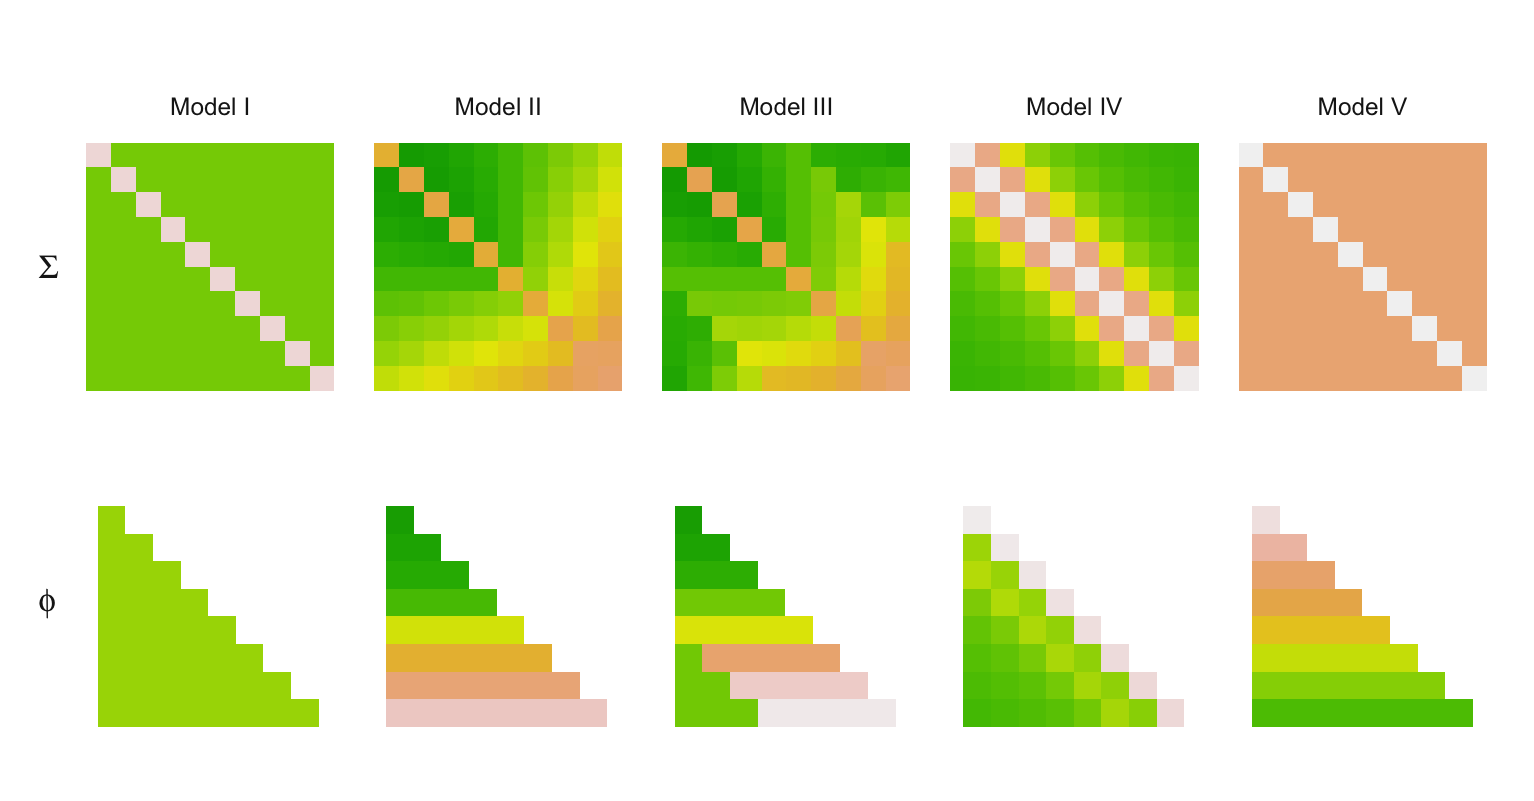
\includegraphics[width = \textwidth]{img/chapter-4/cov-cholesky-grid-beamer}%}
\end{center}

\end{frame}

\begin{frame}{\emph{Simulation Studies}}{Data Generation Settings}

\scriptsize
\begin{center}
\begin{tabular}{lll}
\textbf{I.}  $\Sigma = \mathrm{I}$ & $\phi\left(t,s\right) = 0$, $0 \le s < t \le1$ & $\sigma^2\left(t\right) = 1$, $0 \le  t \le1$\\
\\
\hline
\\
\textbf{II.}  $\Sigma = T^{-1} D {T'}^{-1}$ & $\phi\left(t,s\right) = t - \frac{1}{2},  \;\; 0 \le t \le 1$ & $\sigma^2\left(t\right) = 0.1^2$, $0 \le  t \le1$\\
\\
\hline
\\
\textbf{III.} $\Sigma = T^{-1} D {T'}^{-1}$ & $\phi\left(t,s\right) = \left\{\begin{array}{l} t - \frac{1}{2}, \;\; t - s \le 0.5\\  0, \;\;\;\;\;\; t - s > 0.5\end{array}\right.$ & $\sigma^2\left(t\right) = 0.1^2$, $0 \le  t \le1$ \\
\\
\hline
\\
\textbf{IV.} $\Sigma = \left[\sigma_{ij}\right]$ &   $\sigma_{ij} =\left(1 + \frac{\left(t_i - t_j\right)^2}{2k^2}\right)^{-1} $ & $k = 0.6$, $0 < t_i, t_j < 1$  \\
\\
\hline
\\
\textbf{V.} $\begin{aligned}\Sigma  &= \rho \mathrm{J} + \left(1-\rho\right)\mathrm{I}, \\ &\rho = 0.7 \end{aligned}$ & $\phi_{ts} = \frac{\rho}{1 + \left(t-2\right)\rho}$, $t = 2,\dots, p$ & $ \sigma_t^2 = 1-\frac{\left(\max\left(t,2\right)-2\right)\rho^2}{1 + \left(\max\left(t,2\right)-2\right)\rho}$\\
\end{tabular}
\end{center}


\end{frame}
%
%
%\begin{frame}[c]{\emph{Simulation Studies}}{}
% 
%\begin{center}
% \includegraphics[width = \textwidth]{img/chapter-4/cov-estimate-lattice-beamer}%}
%\end{center}
%
%\end{frame}
%
%
%\begin{frame}[c]{\emph{Simulation Studies}}{}
% 
%\begin{center}
%  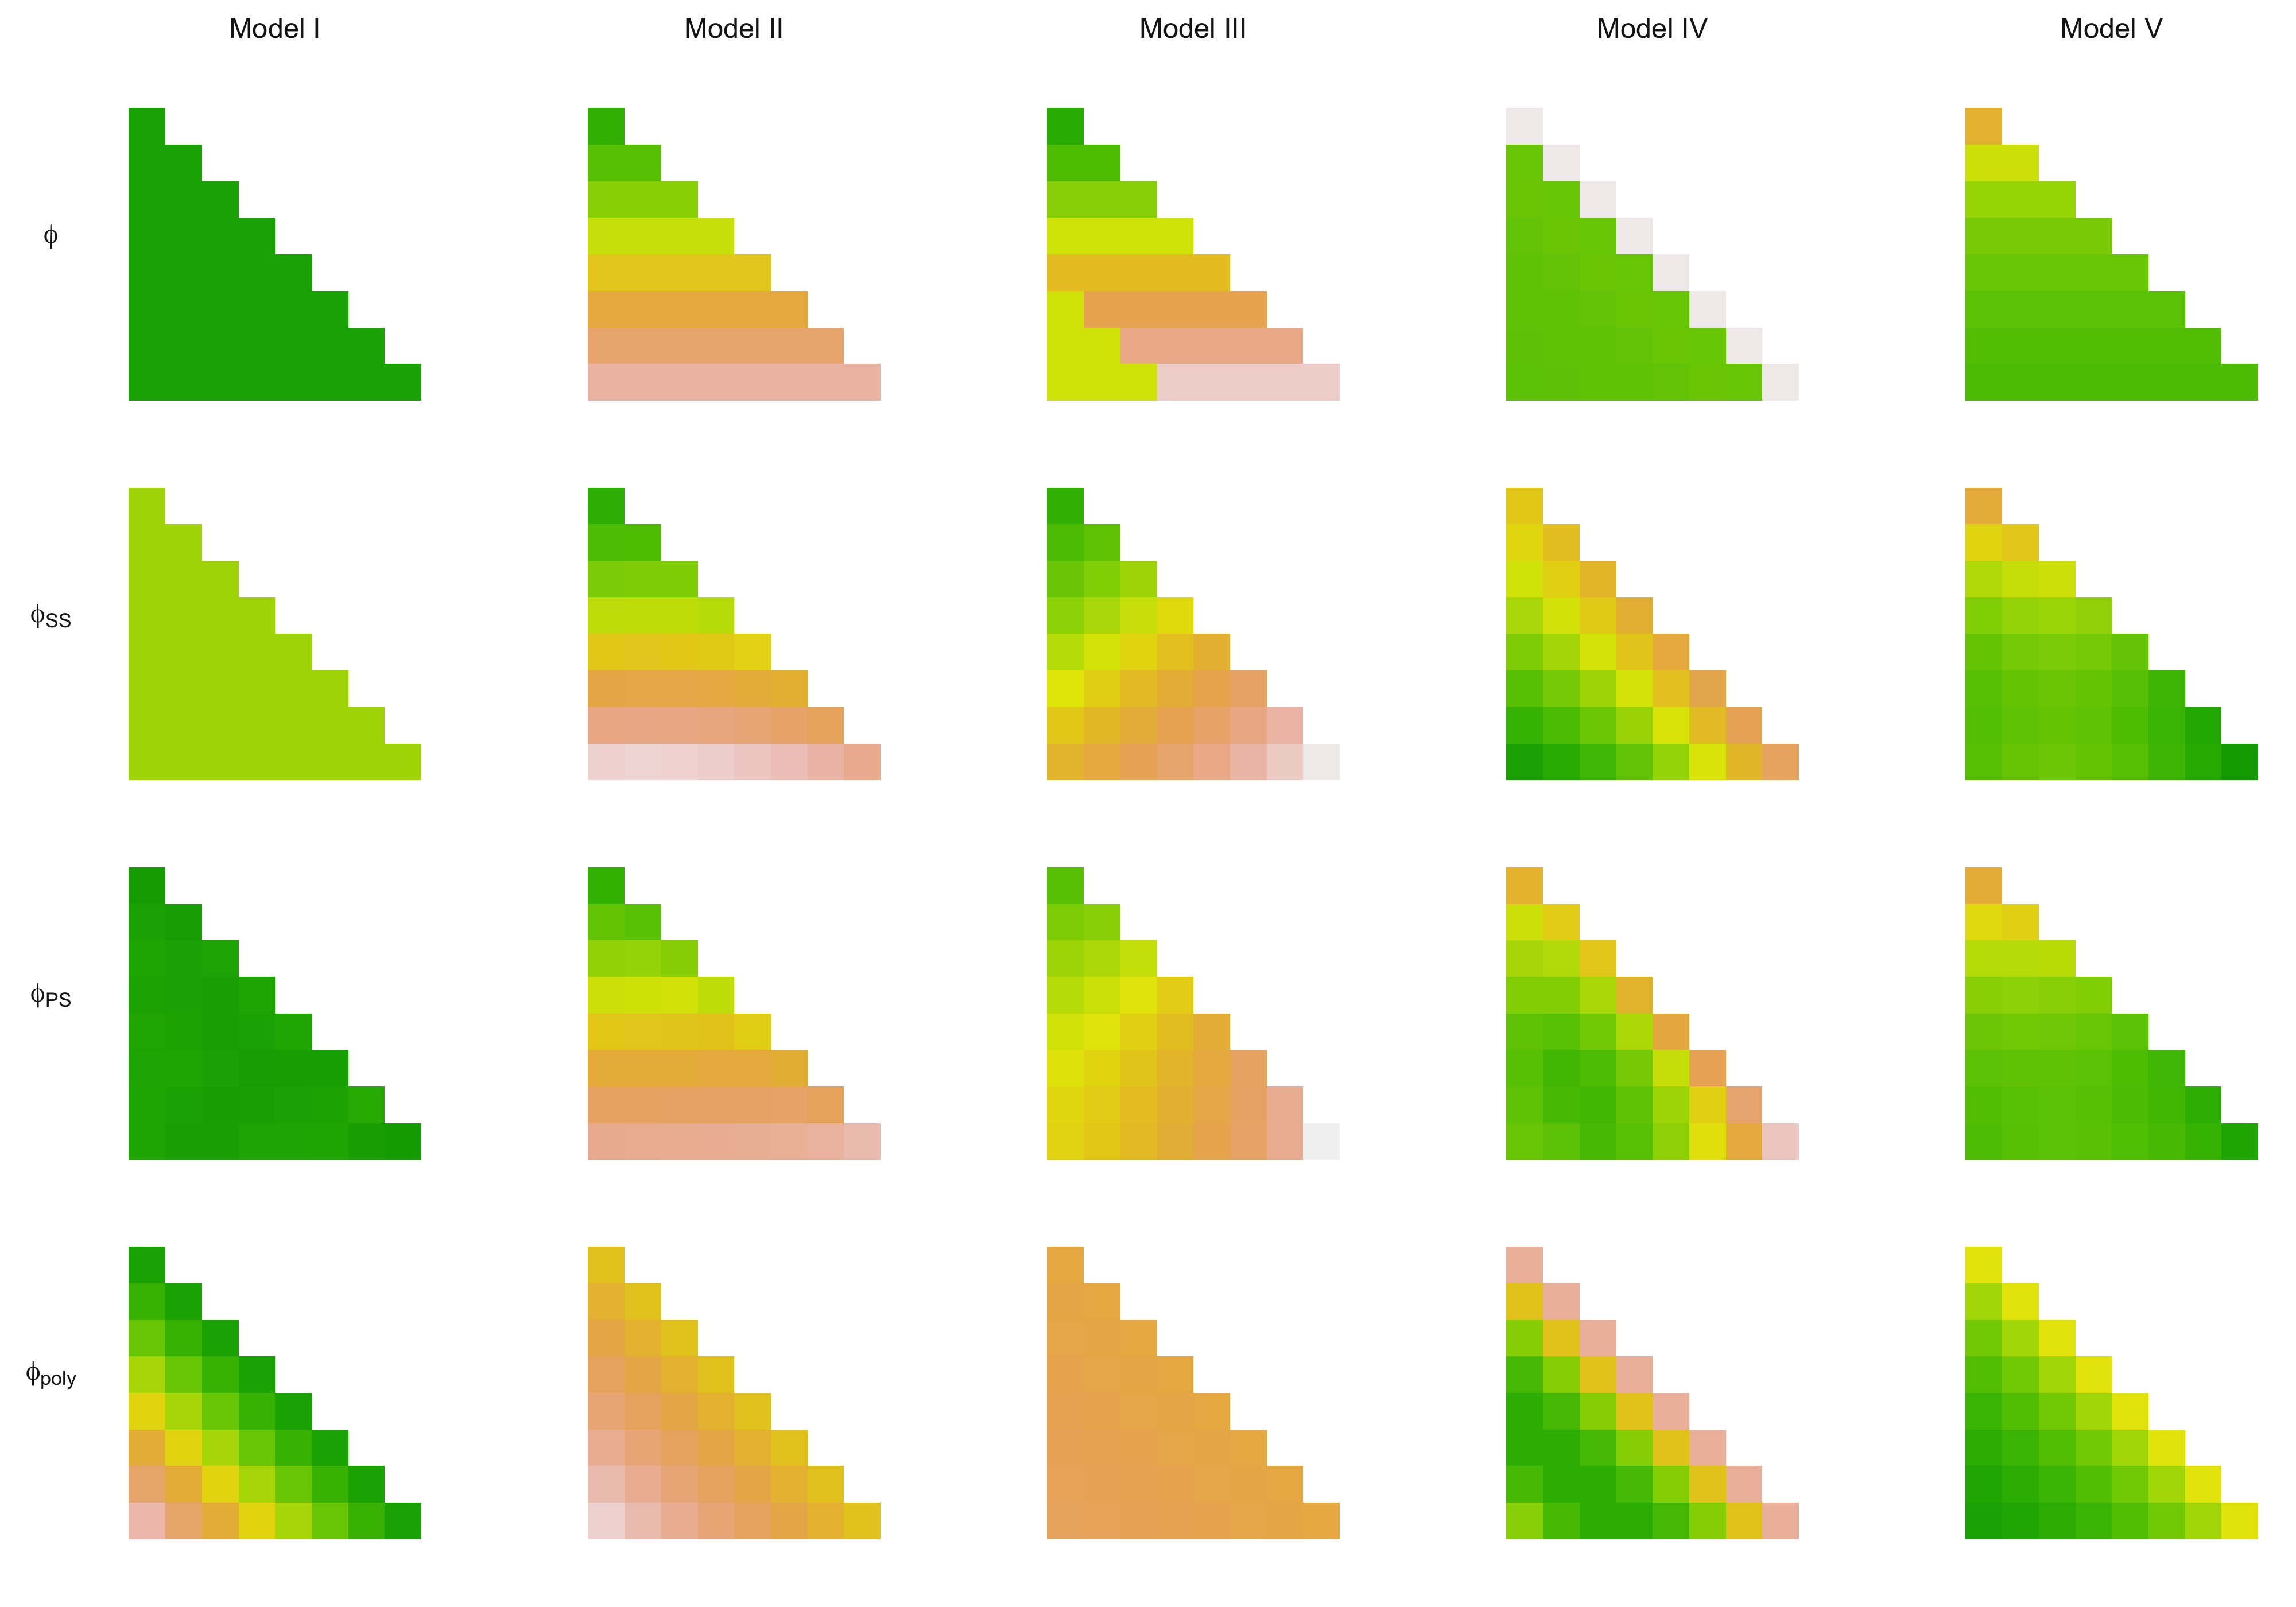
\includegraphics[width = \textwidth]{img/chapter-4/cholesky-estimate-lattice-beamer}%}
%\end{center}
%
%\end{frame}
%
%
%\begin{frame}[c]{\emph{Simulation Studies}}{Results with complete data: Model I}
%\begin{center}
%  \includegraphics[width = \textwidth]{img/chapter-4/model-1-entropy-loss-boxplots}%}
%\end{center}
%\end{frame}
%
%\begin{frame}[c]{\emph{Simulation Studies}}{Results with complete data: Model II}
%\begin{center}
%  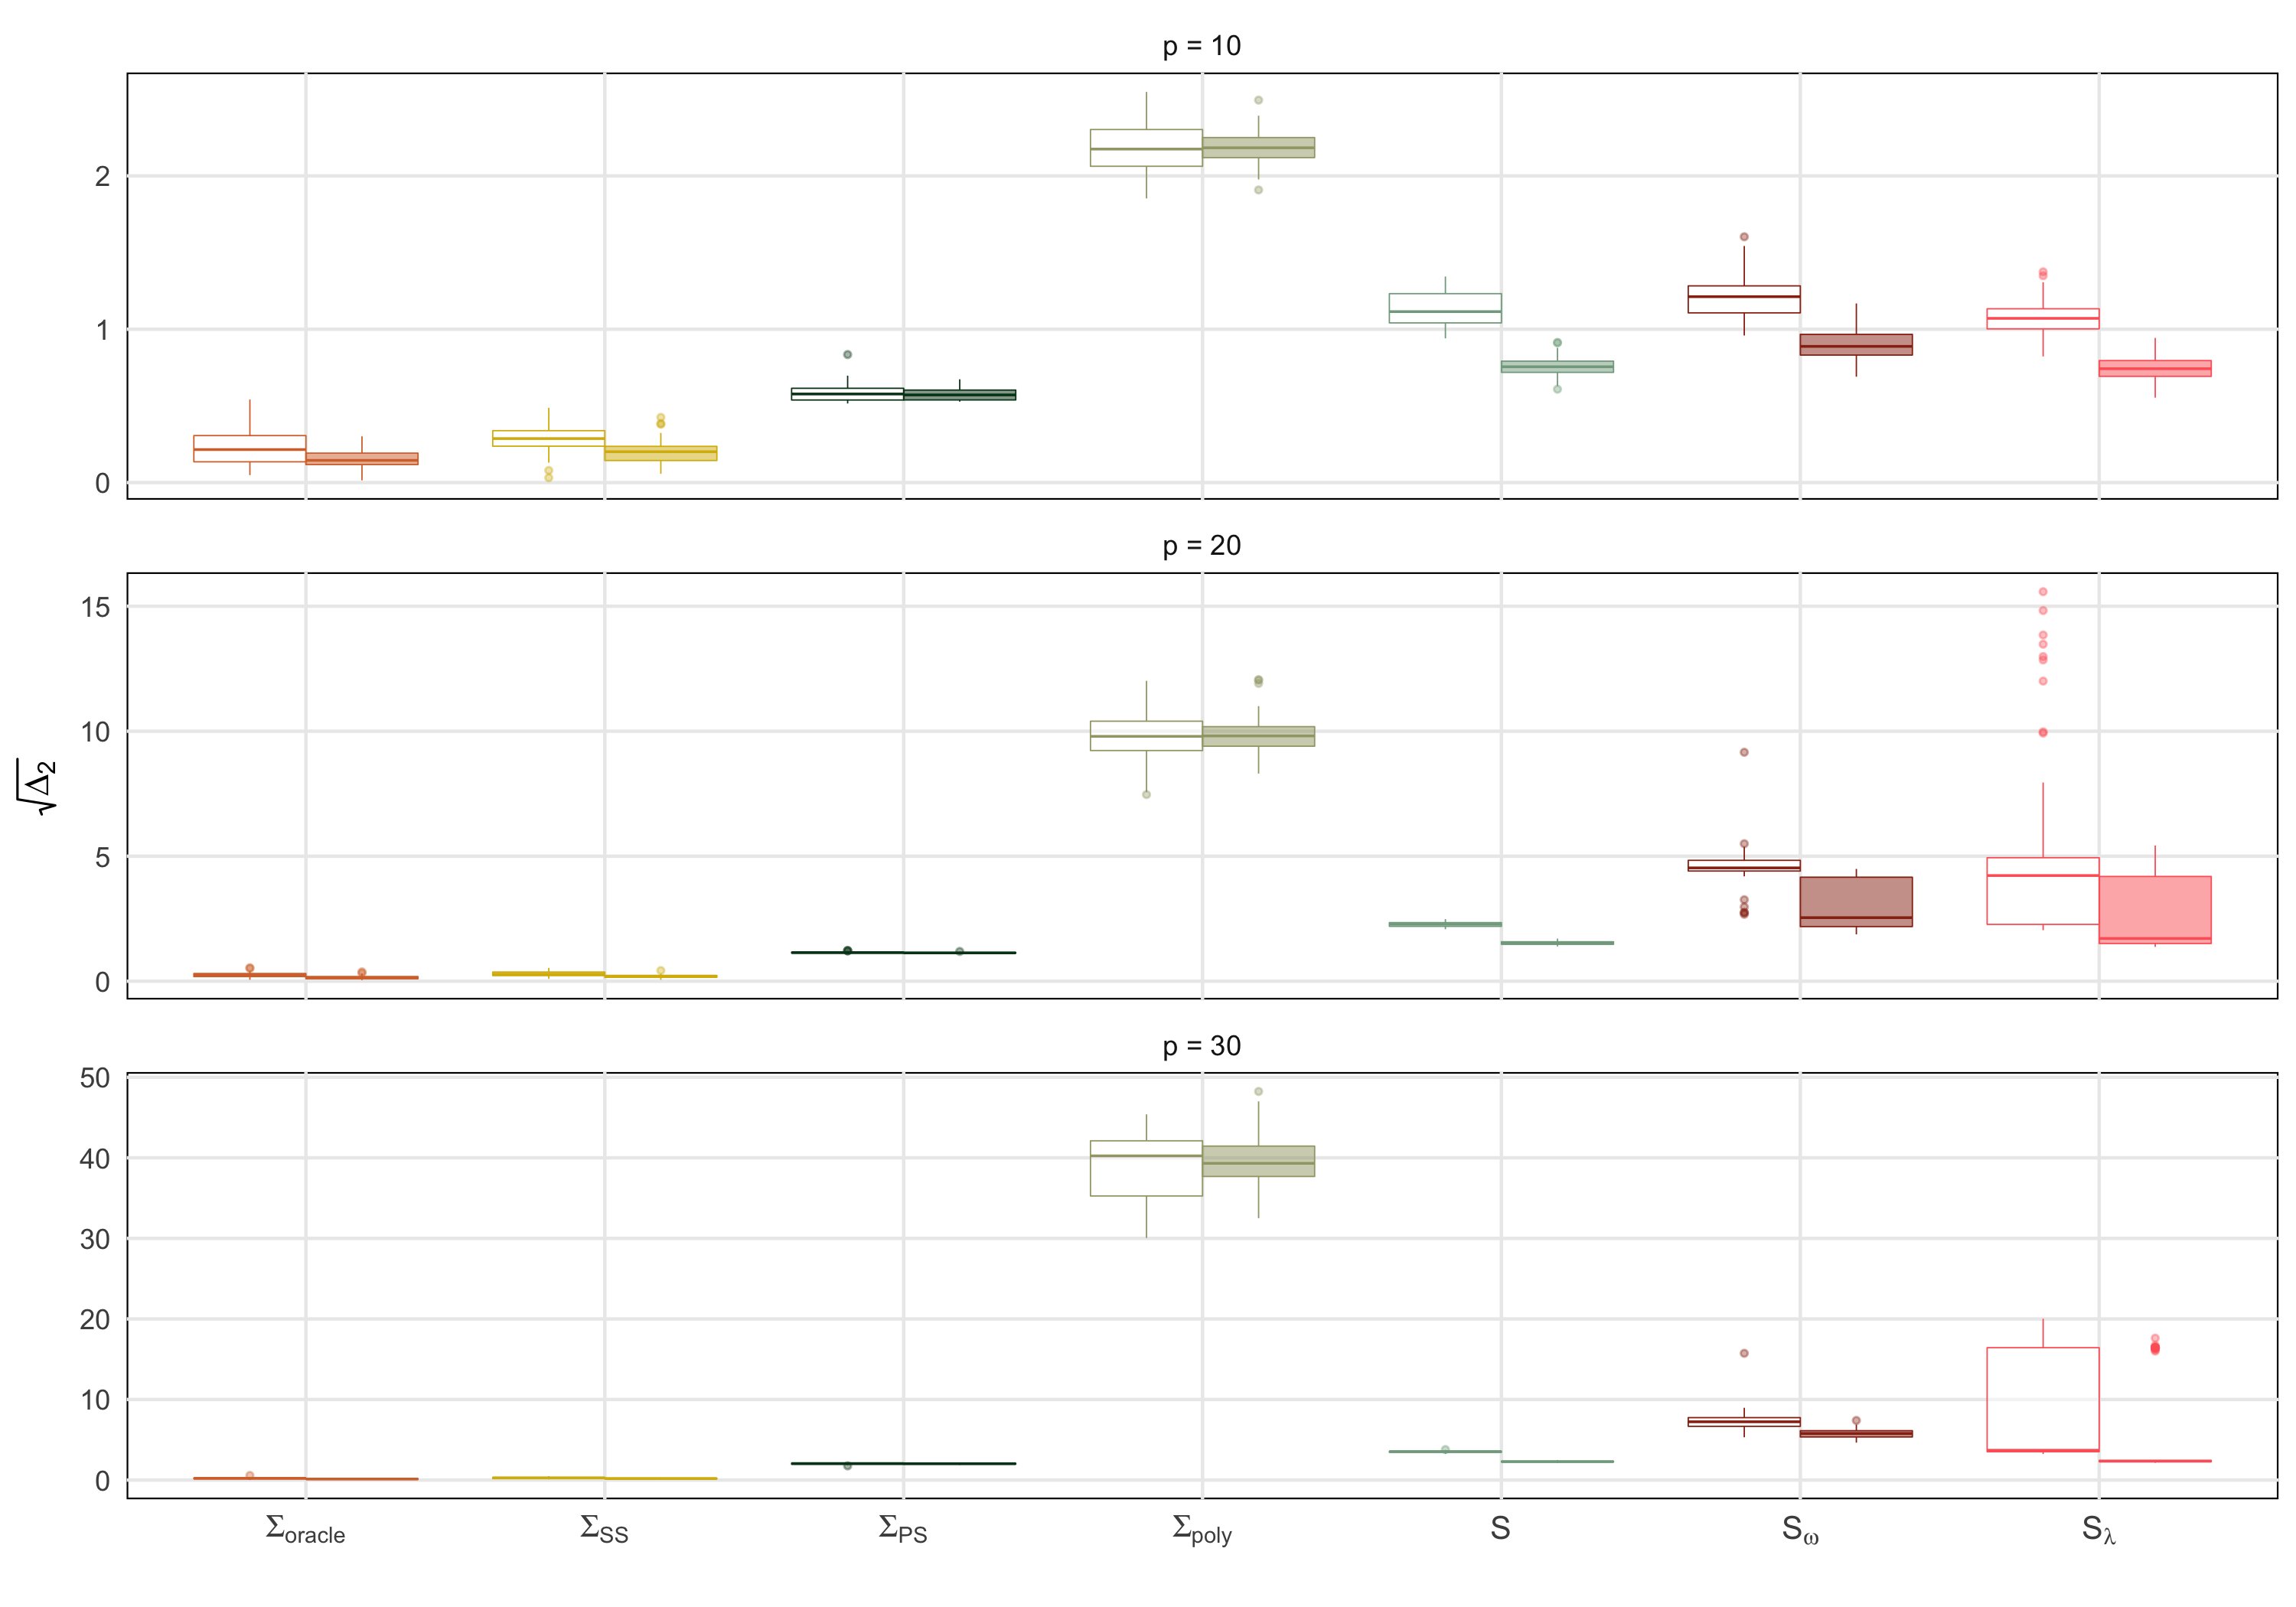
\includegraphics[width = \textwidth]{img/chapter-4/model-2-entropy-loss-boxplots}%}
%\end{center}
%\end{frame}
%
%\begin{frame}[c]{\emph{Simulation Studies}}{Results with complete data: Model III}
%\begin{center}
%  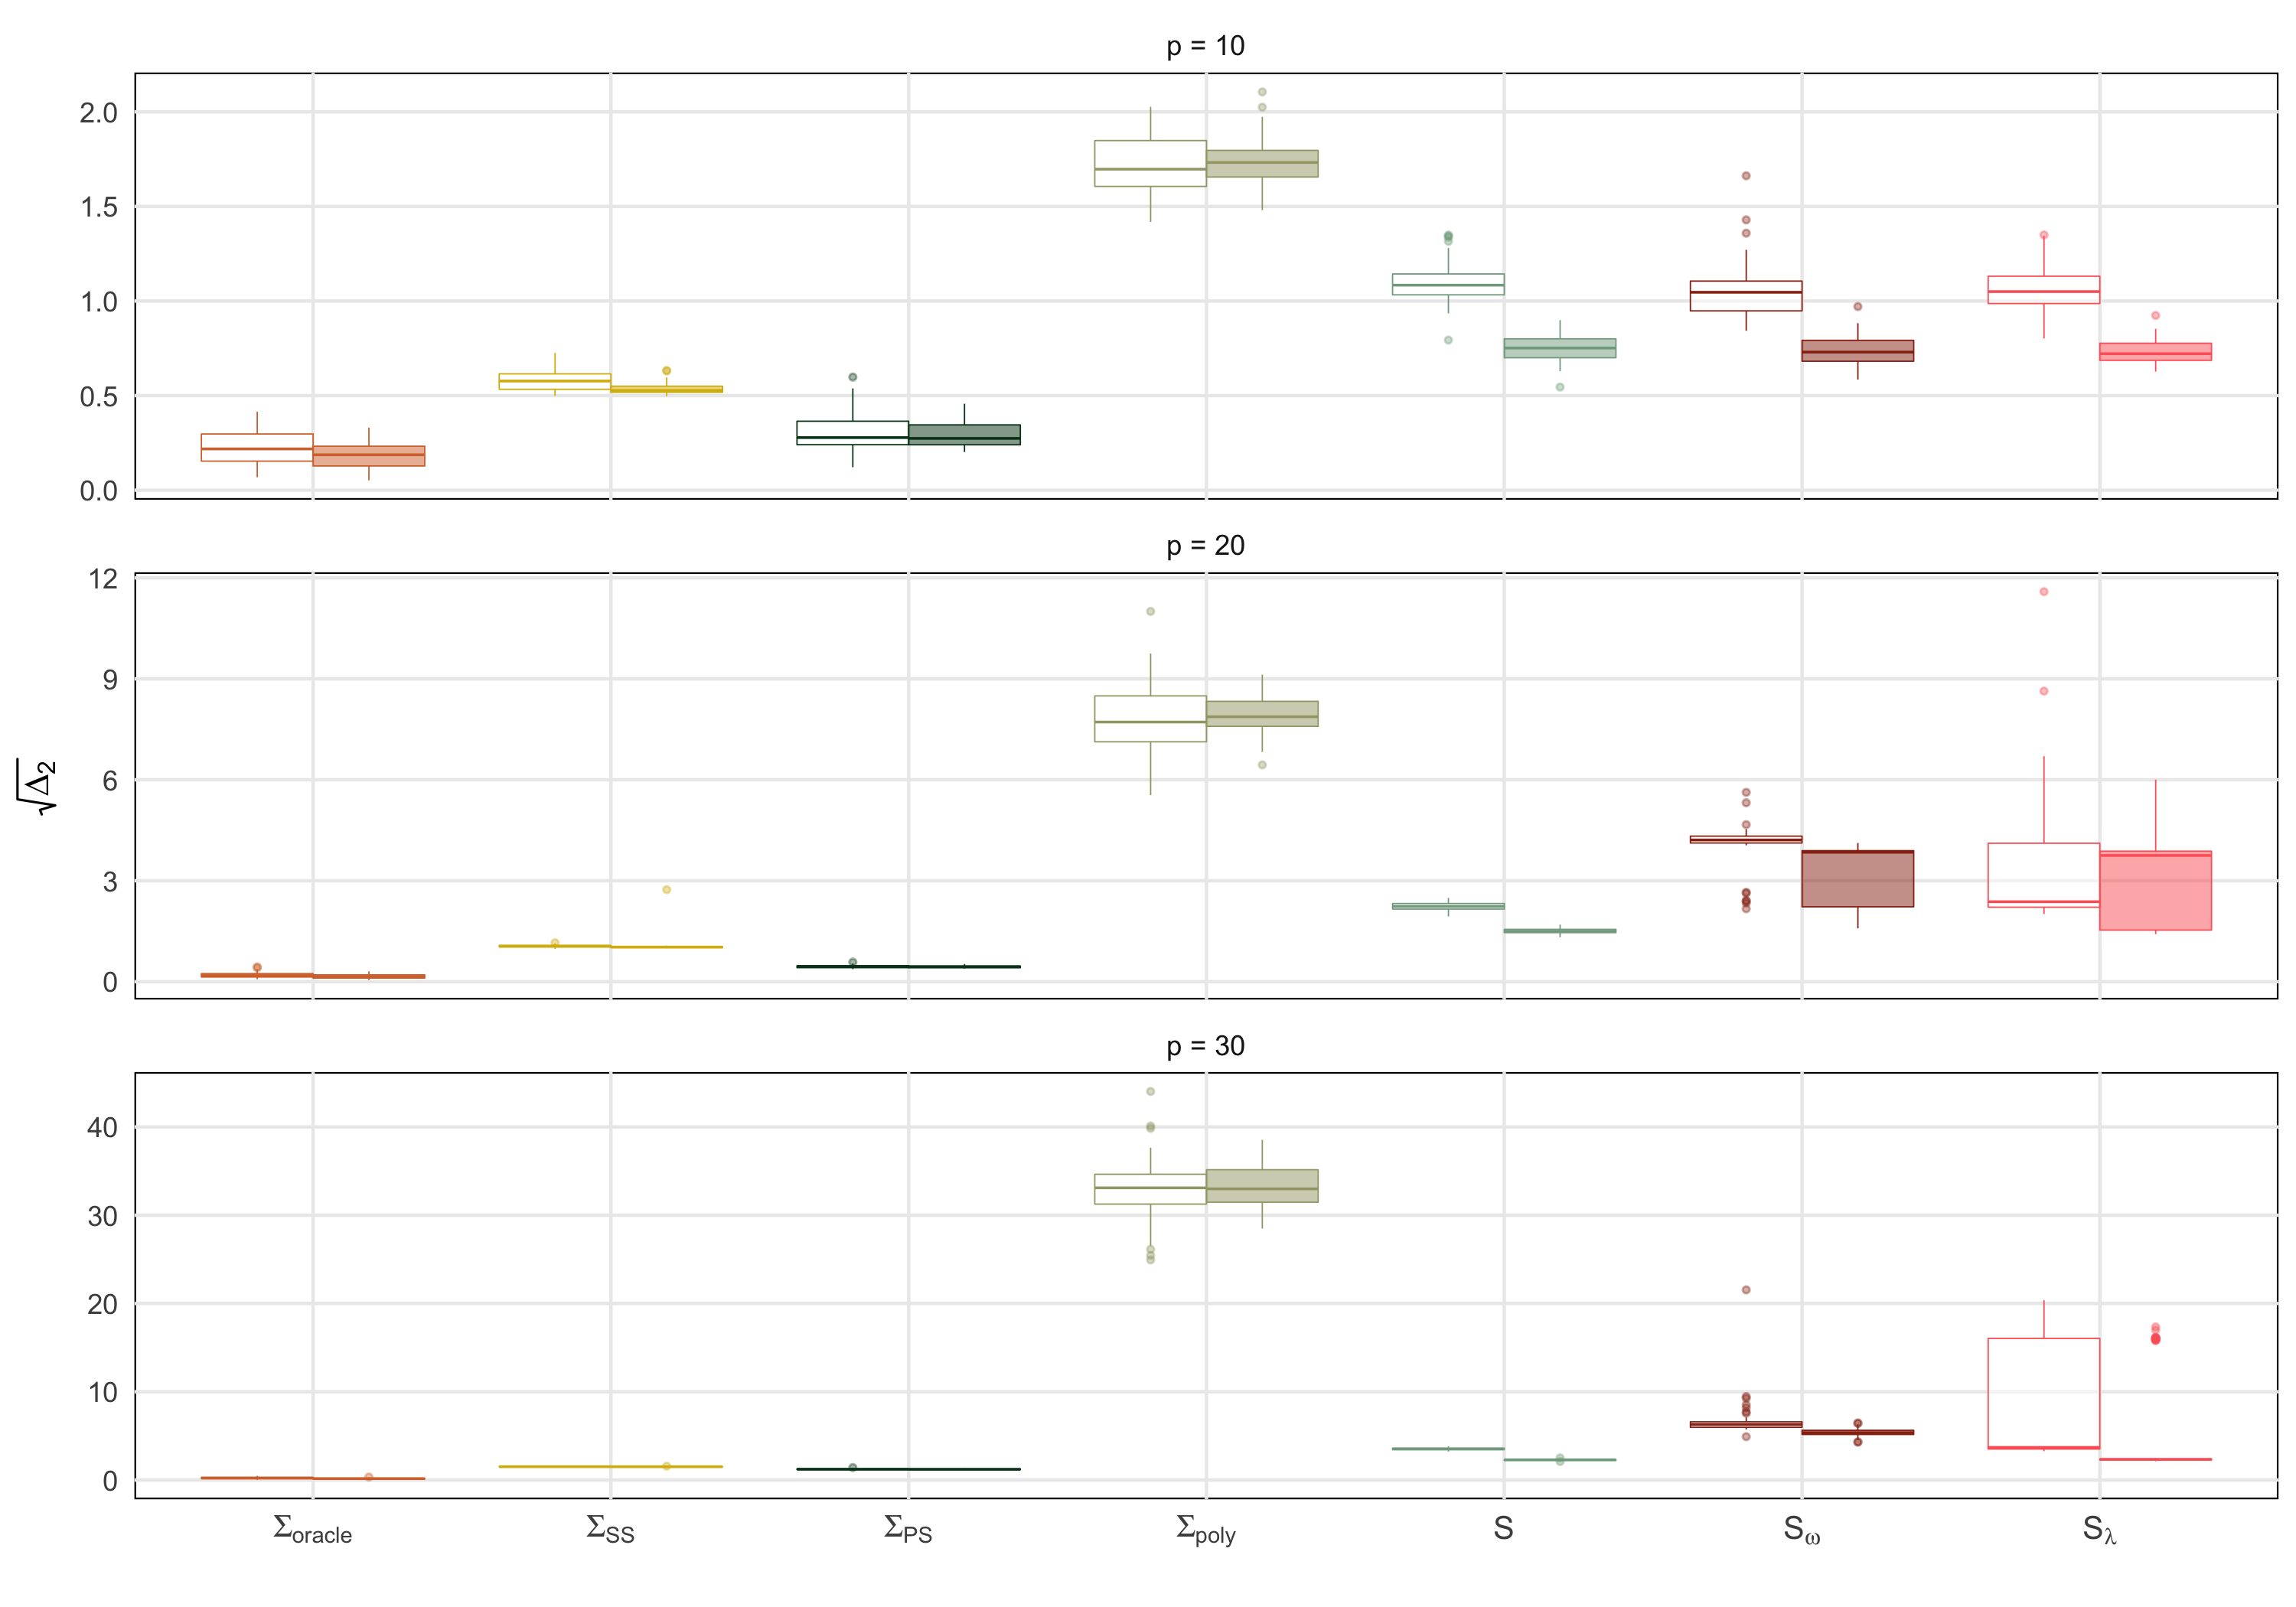
\includegraphics[width = \textwidth]{img/chapter-4/model-3-entropy-loss-boxplots}%}
%\end{center}
%\end{frame}
%
%\begin{frame}[c]{\emph{Simulation Studies}}{Results with complete data: Model IV}
%\begin{center}
%  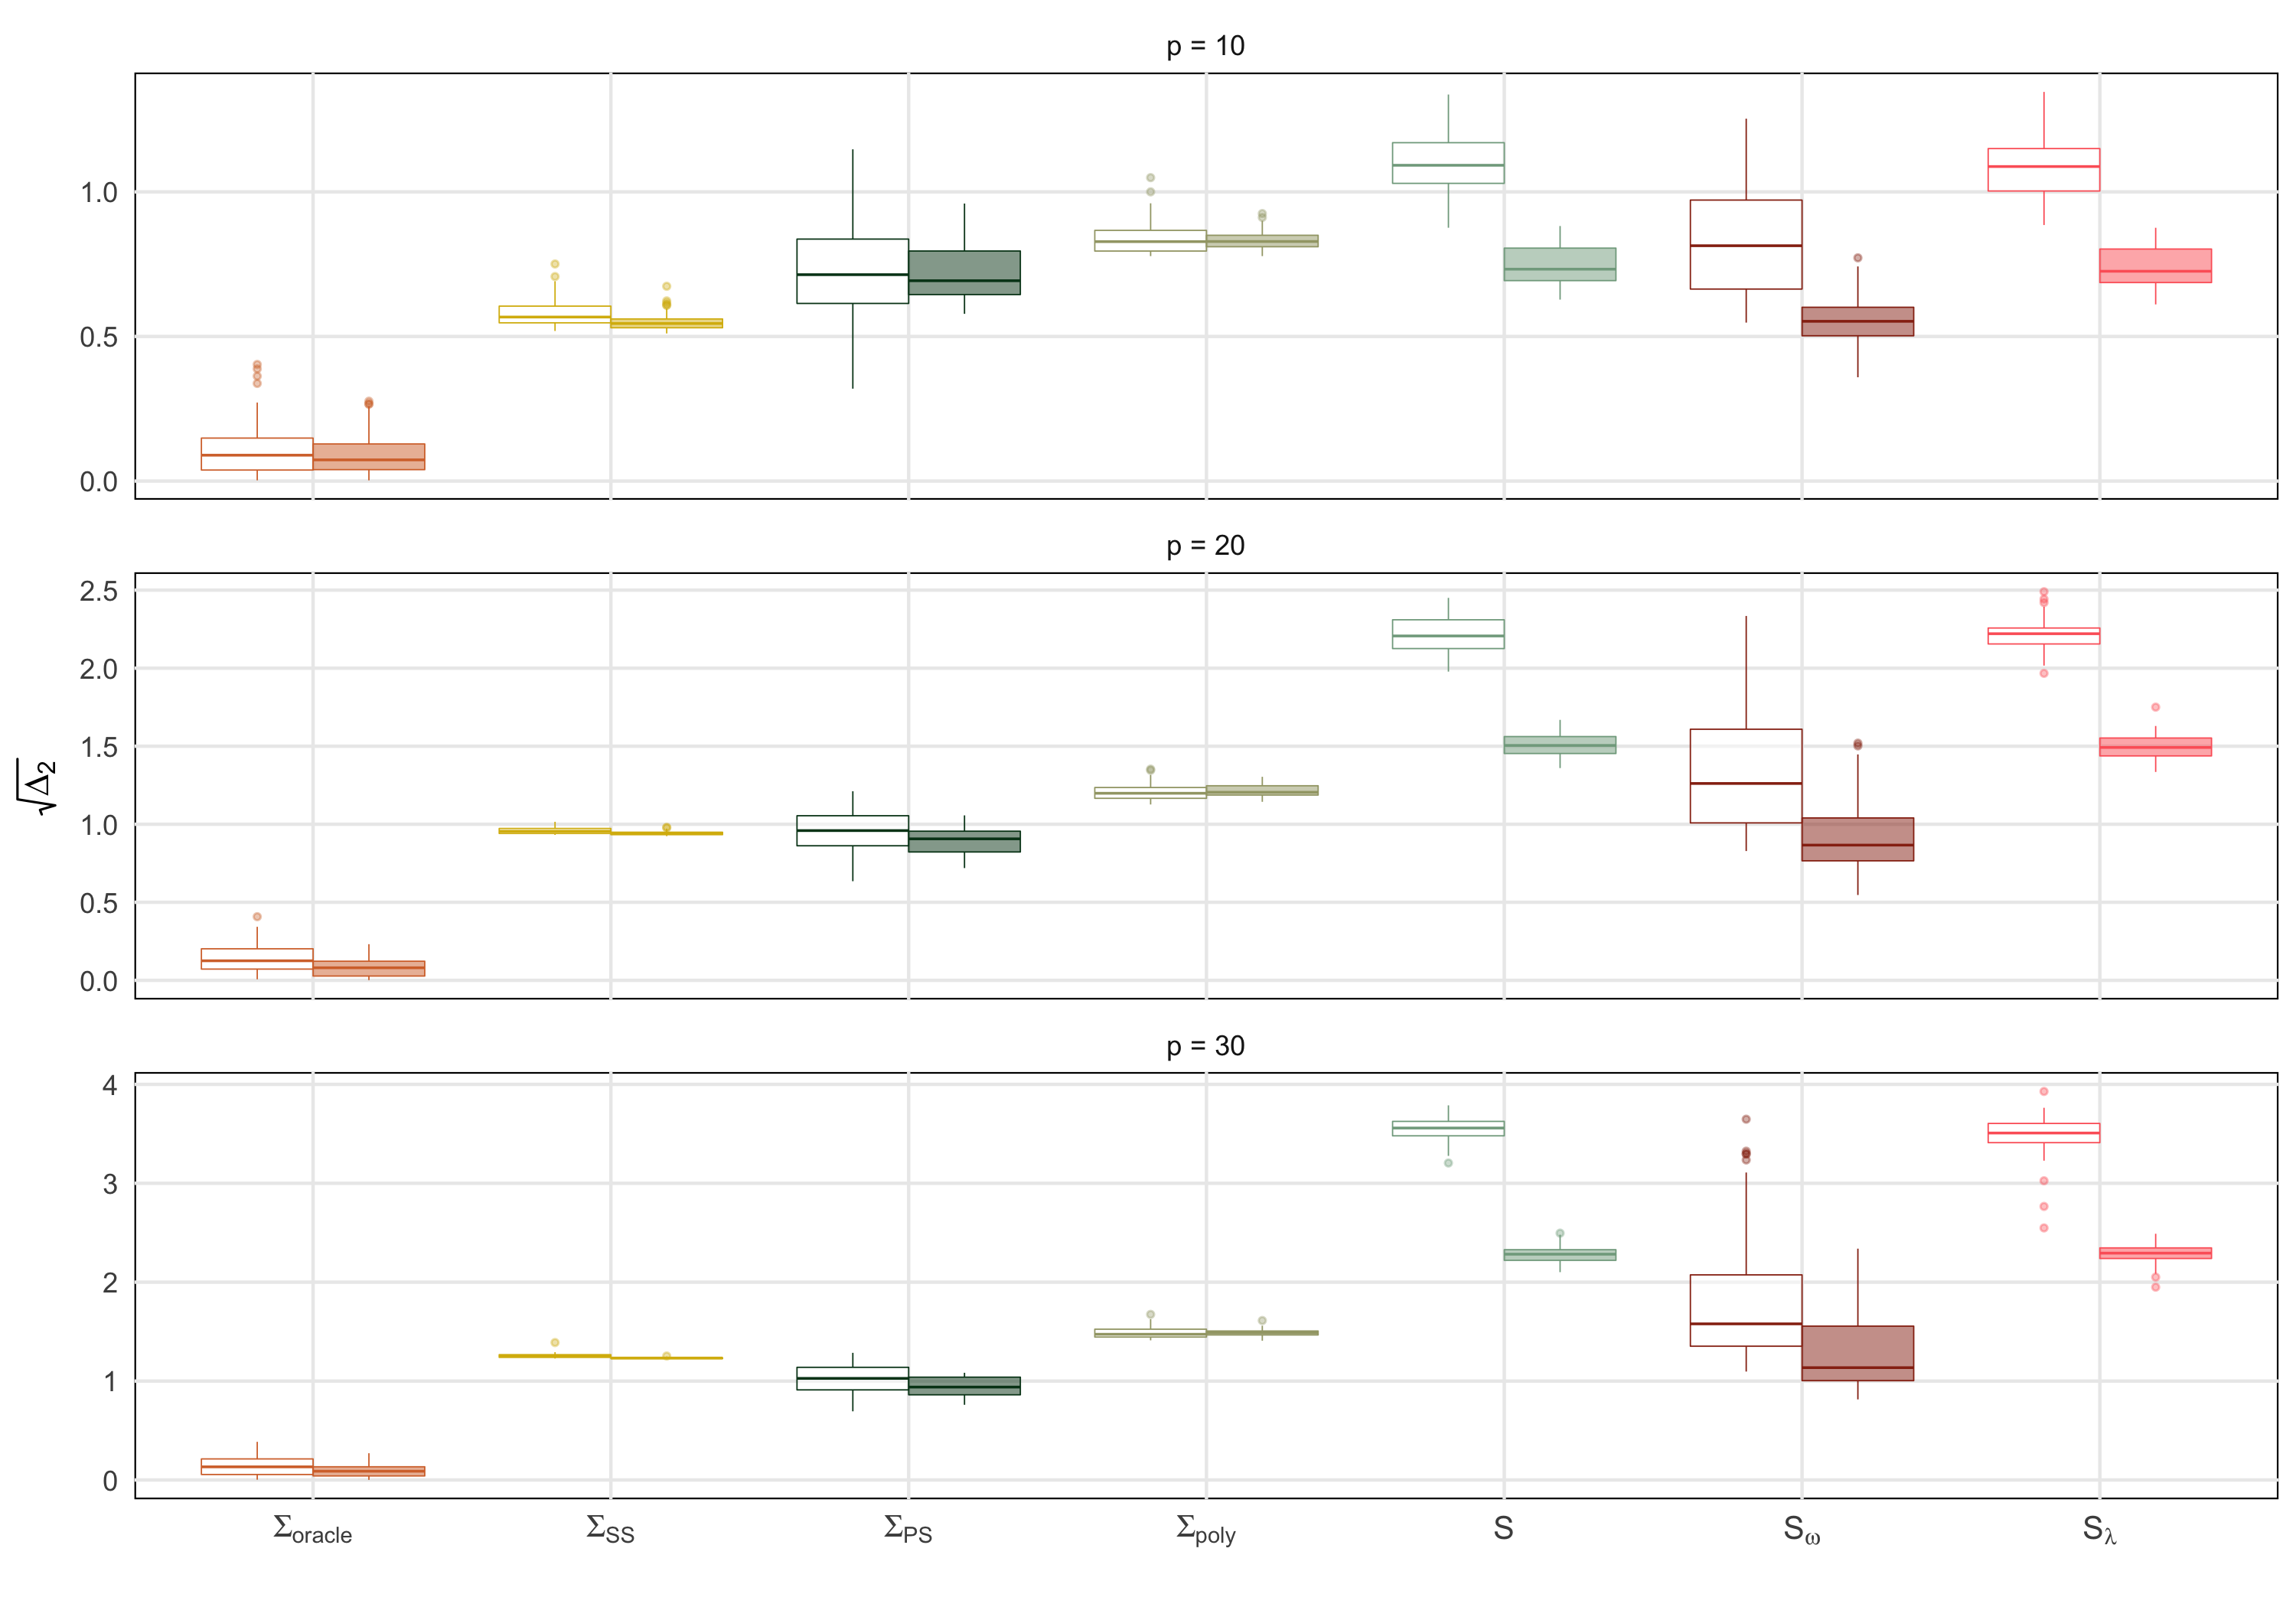
\includegraphics[width = \textwidth]{img/chapter-4/model-4-entropy-loss-boxplots}%}
%\end{center}
%\end{frame}
%
%\begin{frame}[c]{\emph{Simulation Studies}}{Results with complete data: Model V}
%\begin{center}
%  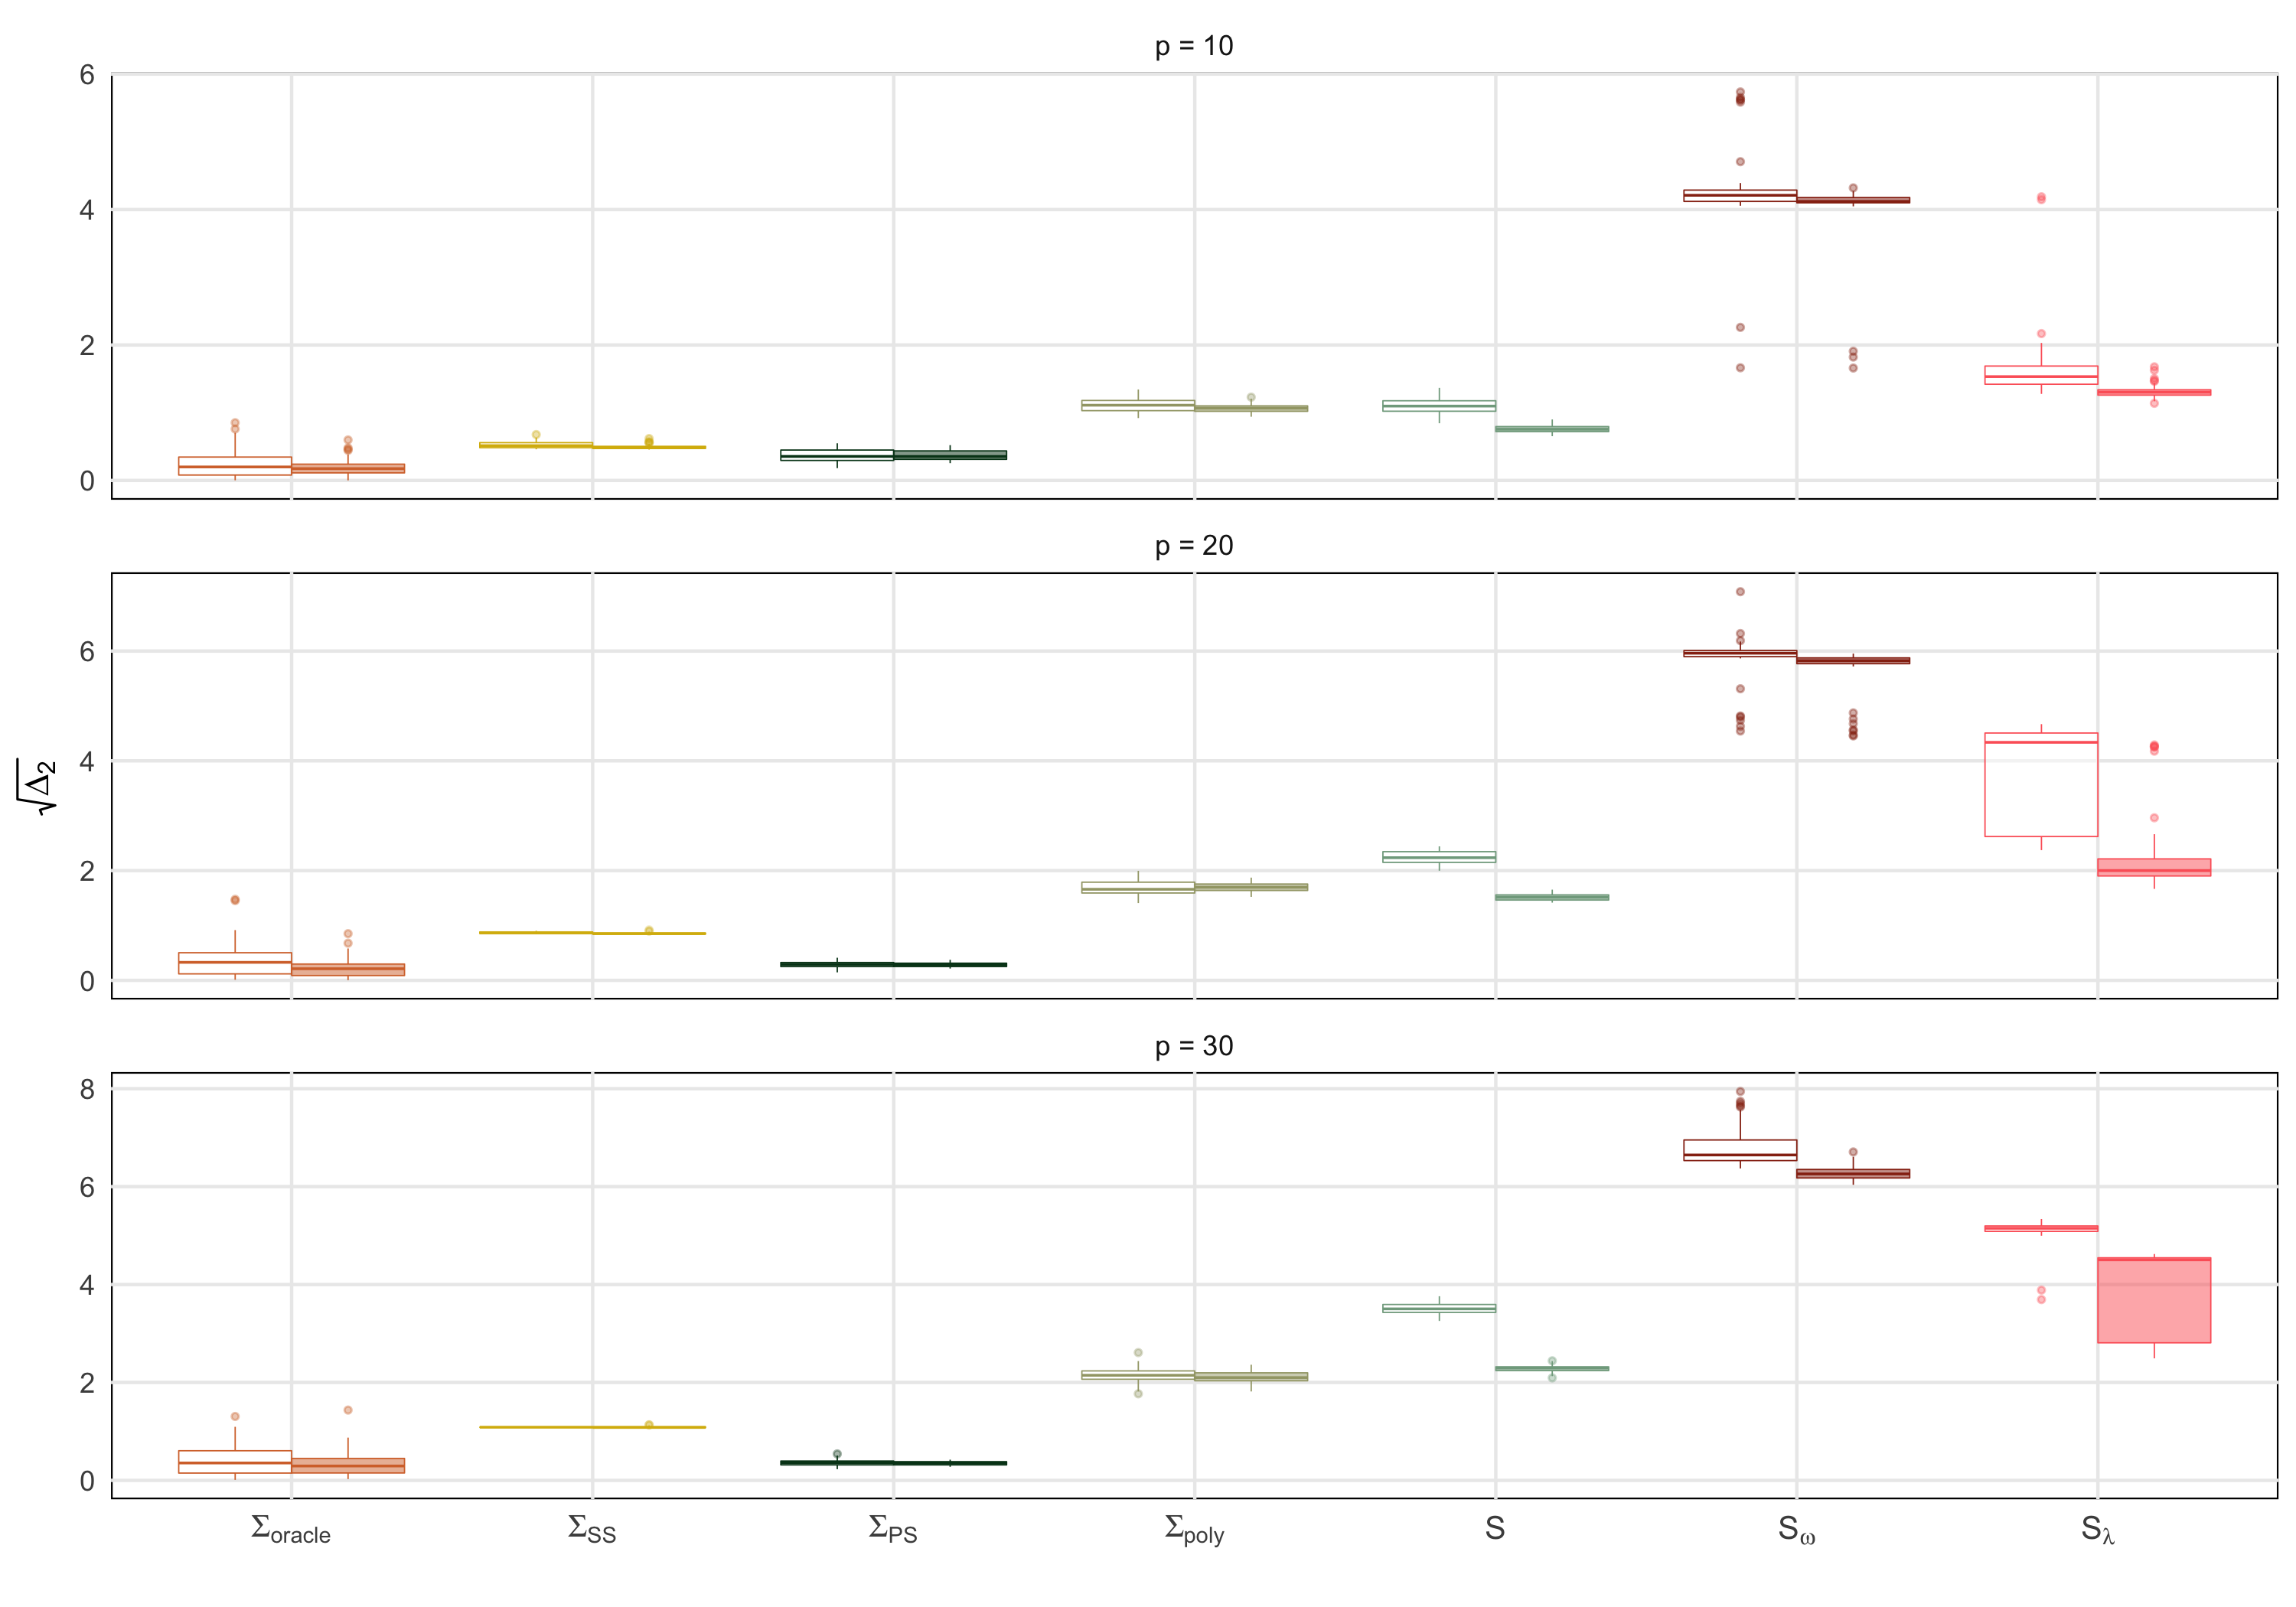
\includegraphics[width = \textwidth]{img/chapter-4/model-5-entropy-loss-boxplots}%}
%\end{center}
%\end{frame}
%
%\begin{frame}[c]{\emph{Simulation Studies}}{Results with complete data: Model V}
%\begin{center}
%  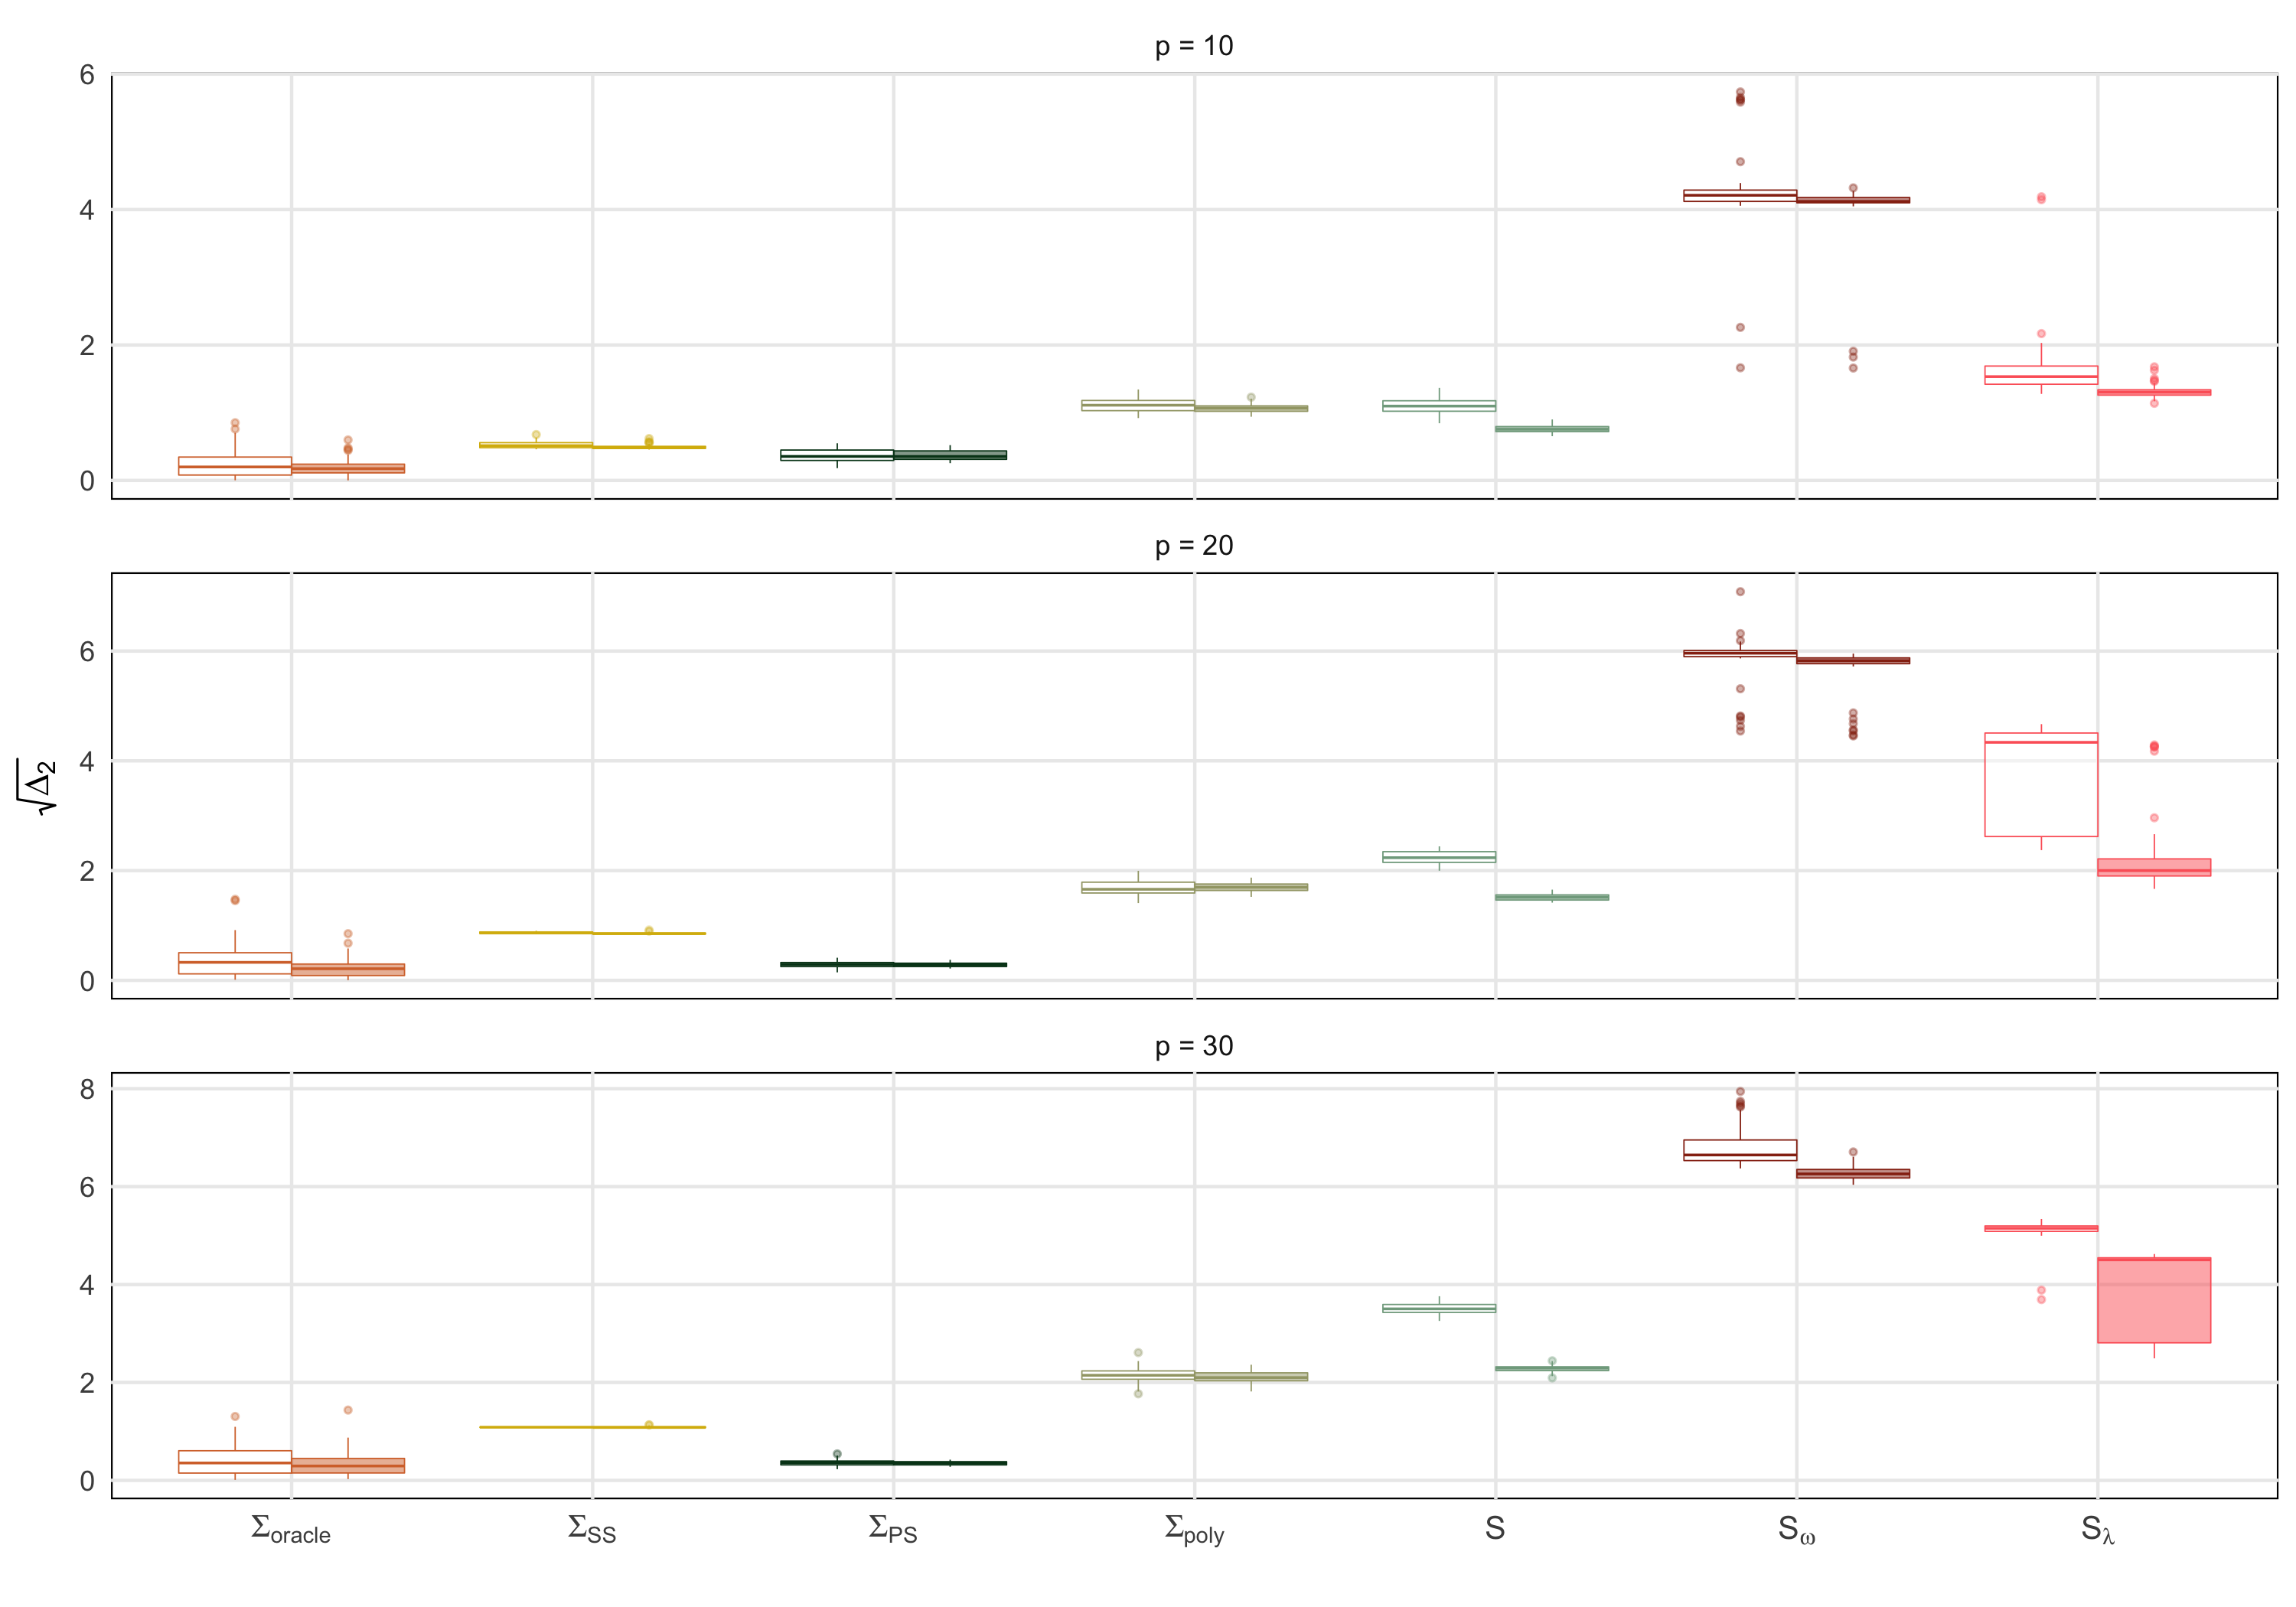
\includegraphics[width = \textwidth]{img/chapter-4/model-5-entropy-loss-boxplots}%}
%\end{center}
%\end{frame}
%
%\begin{frame}[c]{\emph{Simulation Studies}}{Simulations with missing data}
%\begin{center}
%  \includegraphics[width = \textwidth]{img/chapter-4/simulation-study-2-entropy-loss-boxplots}
%\end{center}
%\end{frame}
%

%%%%%%%%%%%%%%%%%%%%%%%%%%%%%%%%%%%%%%%%%%%%%%%%%%%%%%%%%%%%%%%%%%%%%%%%%%%%
%%%%%%%%%%%%%%%%%%%%%%%%%%%%%%%%%%%%%%%%%%%%%%%%%%%%%%%%%%%%%%%%%%%%%%%%%%%%
%%%%%%%%%%%%%%%%%%%%%%%%%%%%%%%%%%%%%%%%%%%%%%%%%%%%%%%%%%%%%%%%%%%%%%%%%%%%
%%%%%%%%%%%%%%%%%%%%%%%%%%%%%%%%%%%%%%%%%%%%%%%%%%%%%%%%%%%%%%%%%%%%%%%%%%%%



\begin{frame}[c]{\textit{Kenward Cattle Data}}

\begin{center}
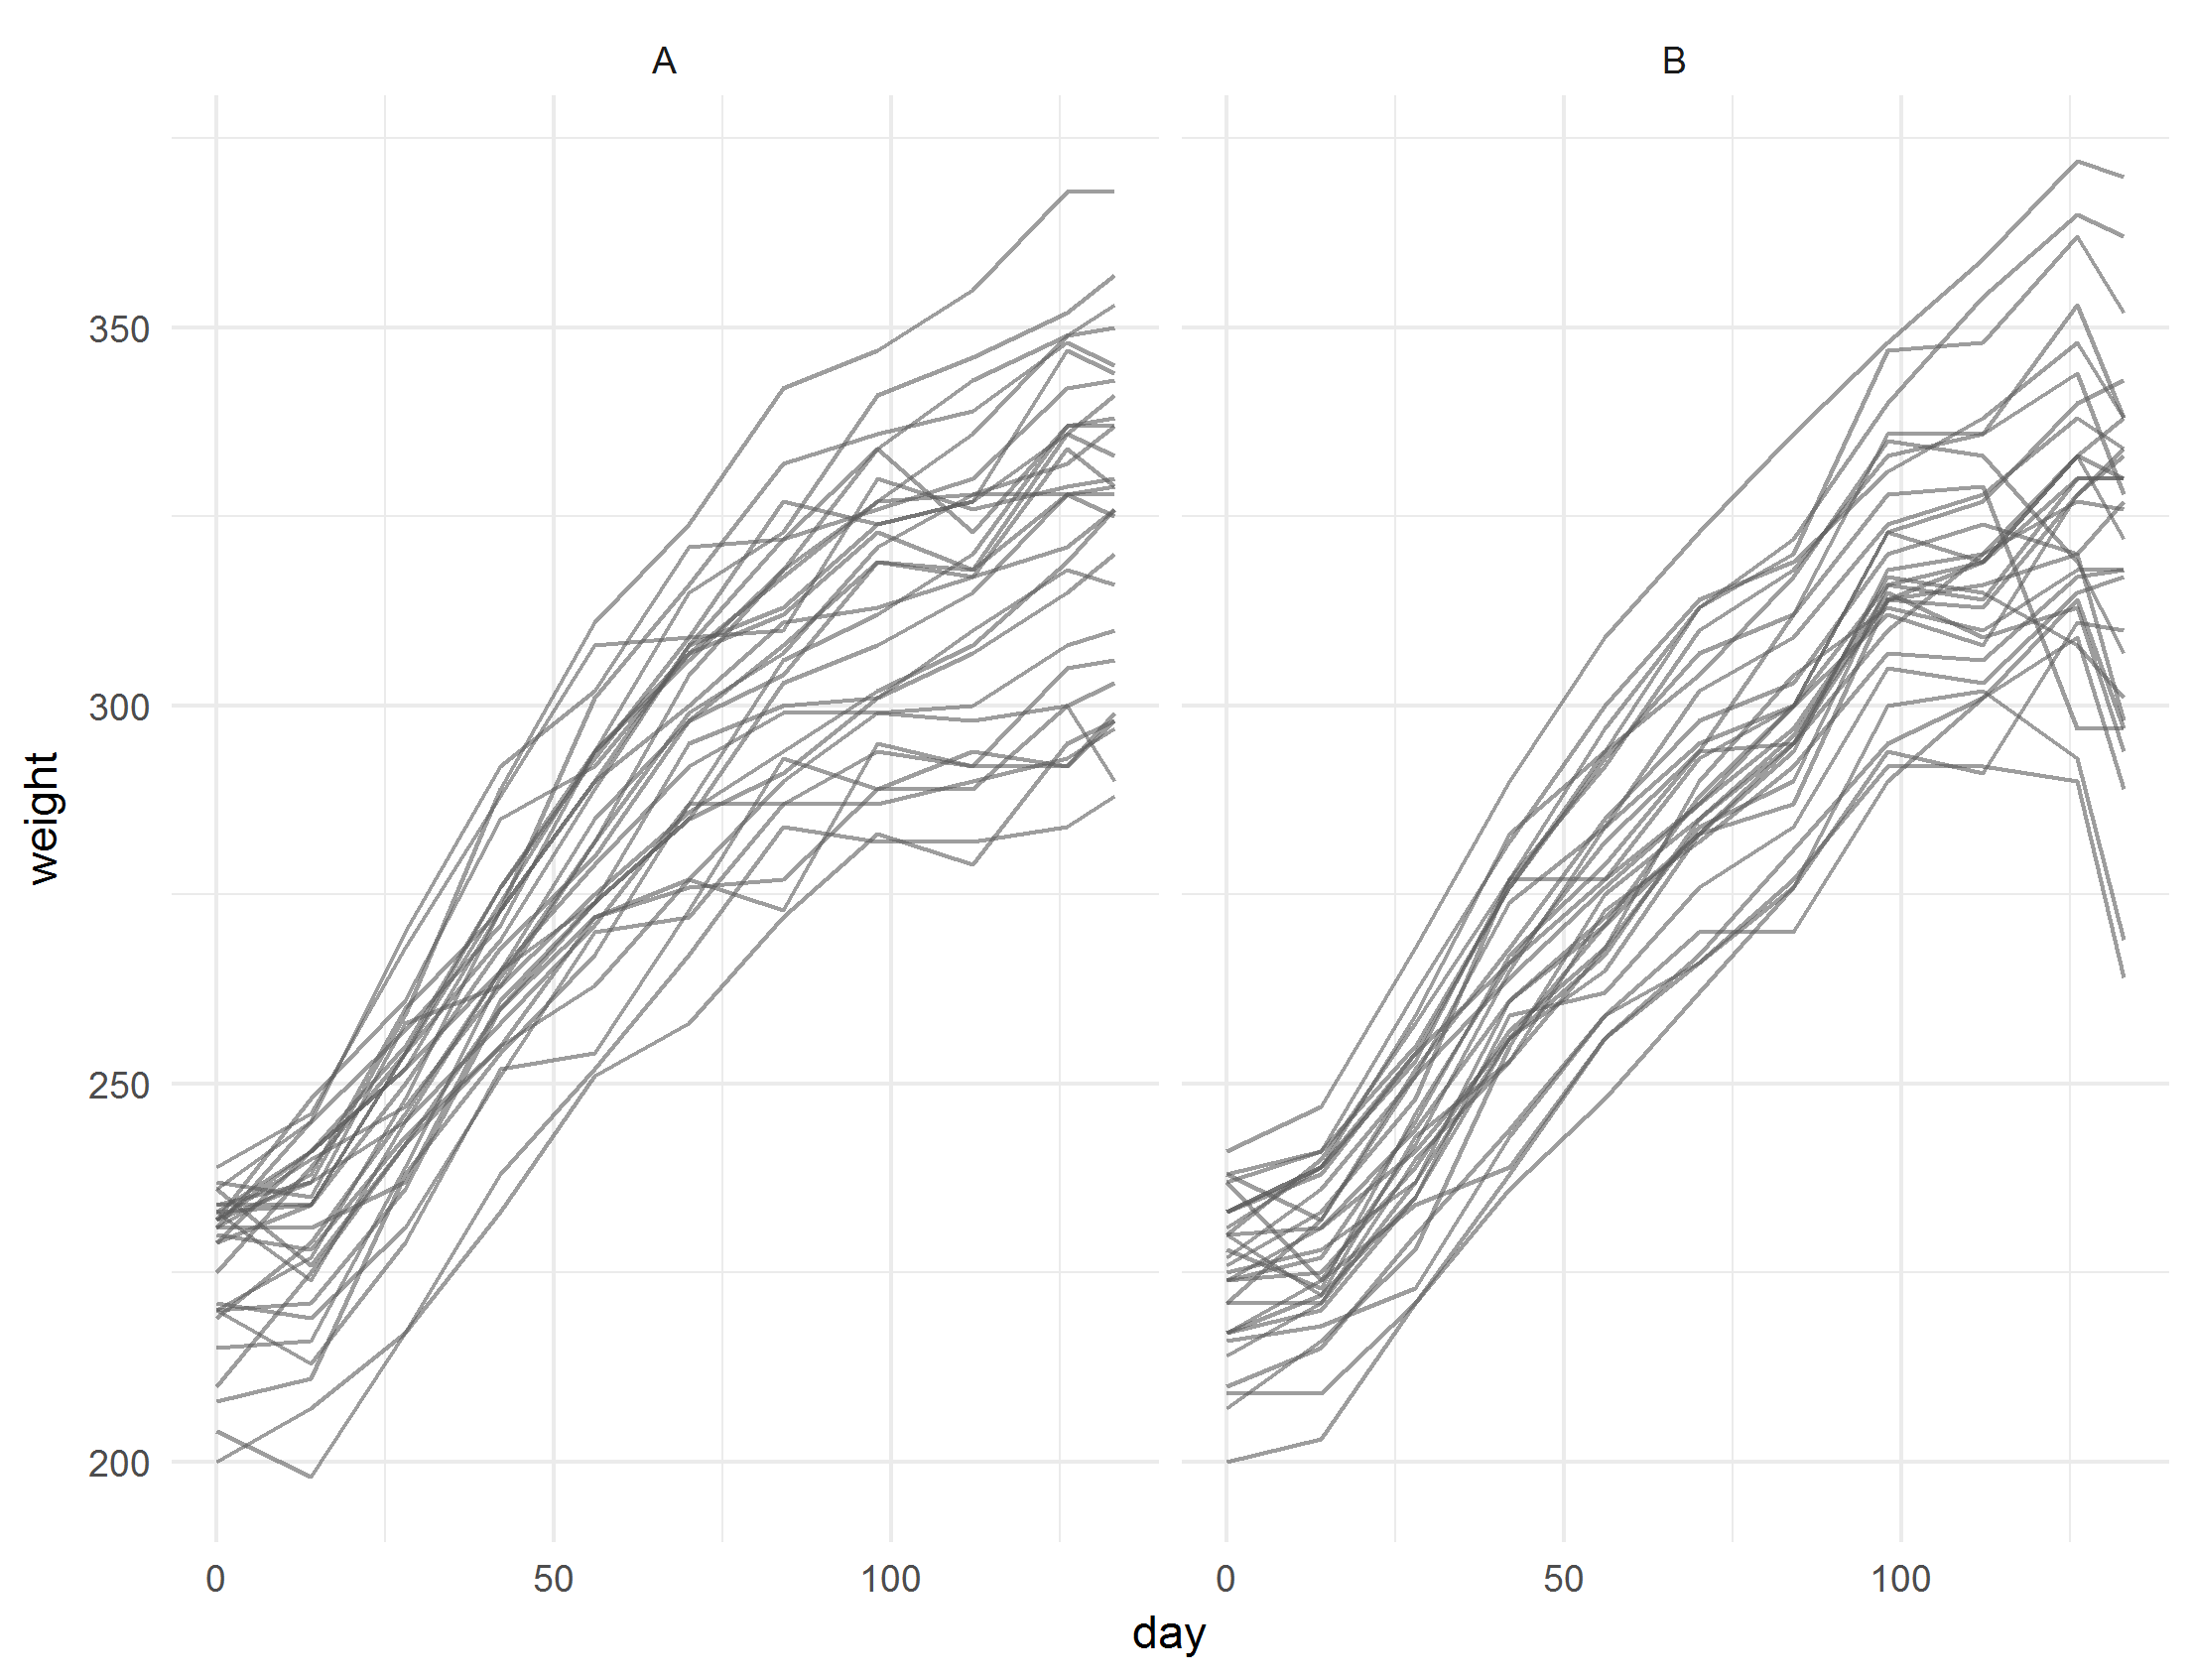
\includegraphics[width = .9\textwidth]{img/cattle/cattle-weights-vs-time-by-trt}
%\caption{\textit{Subject-specific weight curves over time for treatment groups A and B.}}\label{fig:cattle-weights-by-trt}
\end{center}
\end{frame}


\begin{frame}[c]{\textit{Kenward Cattle Data}}{Sample correlations}
\begin{center}
%\begin{table}
\scriptsize
\begin{tabular}{r|rrrrrrrrrrr}
& \multicolumn{11}{c}{day}\\
&&&&&&&&&&\\
& 0 & 14 & 28 & 42 & 56 & 70 & 84 & 98& 112& 126 &133\\
  \hline\noalign{\smallskip} 
0 & 1.00  \\ 
  14 & 0.82 & 1.00  \\ 
  28 & 0.76 & 0.91 & 1.00 & \\ 
  42 & 0.65 & 0.86 & 0.93 & 1.00 &  \\ 
  56 & 0.63 & 0.83 & 0.89 & 0.93 & 1.00 &  \\ 
  70 & 0.58 & 0.75 & 0.85 & 0.90 & 0.94 & 1.00 & \\ 
  84 & 0.51 & 0.64 & 0.75 & 0.80 & 0.85 & 0.92 & 1.00 &\\ 
  98 & 0.52 & 0.68 & 0.77 & 0.82 & 0.88 & 0.93 & 0.92 & 1.00 & \\ 
  112 & 0.51 & 0.61 & 0.71 & 0.74 & 0.81 & 0.89 & 0.92 & 0.96 & 1.00 & \\ 
  120 & 0.46 & 0.59 & 0.69 & 0.70 & 0.77 & 0.85 & 0.86 & 0.94 & 0.96 & 1.00 &  \\ 
  133 & 0.46 & 0.56 & 0.67 & 0.67 & 0.74 & 0.81 & 0.84 & 0.91 & 0.95 & 0.98 & 1.00 \\ 
   \hline
\end{tabular}
\end{center}
%\caption{\textit{Cattle data: treatment group A sample correlations.}}\label{table:cattleA-sample-correlations}
%\end
\end{frame}


\begin{frame}{\textit{The regressogram and innovation variogram}}{}
\begin{columns}
\begin{column}[b]{5.5cm}
  \centering
\begin{tikzpicture}%[show background grid] %% Use grid for positioning, then turn off
		% \node[right] at (.5,8) {\comment{\ECFAugie(Left of this ruled out)}};
		\node[right]  at (0,4) {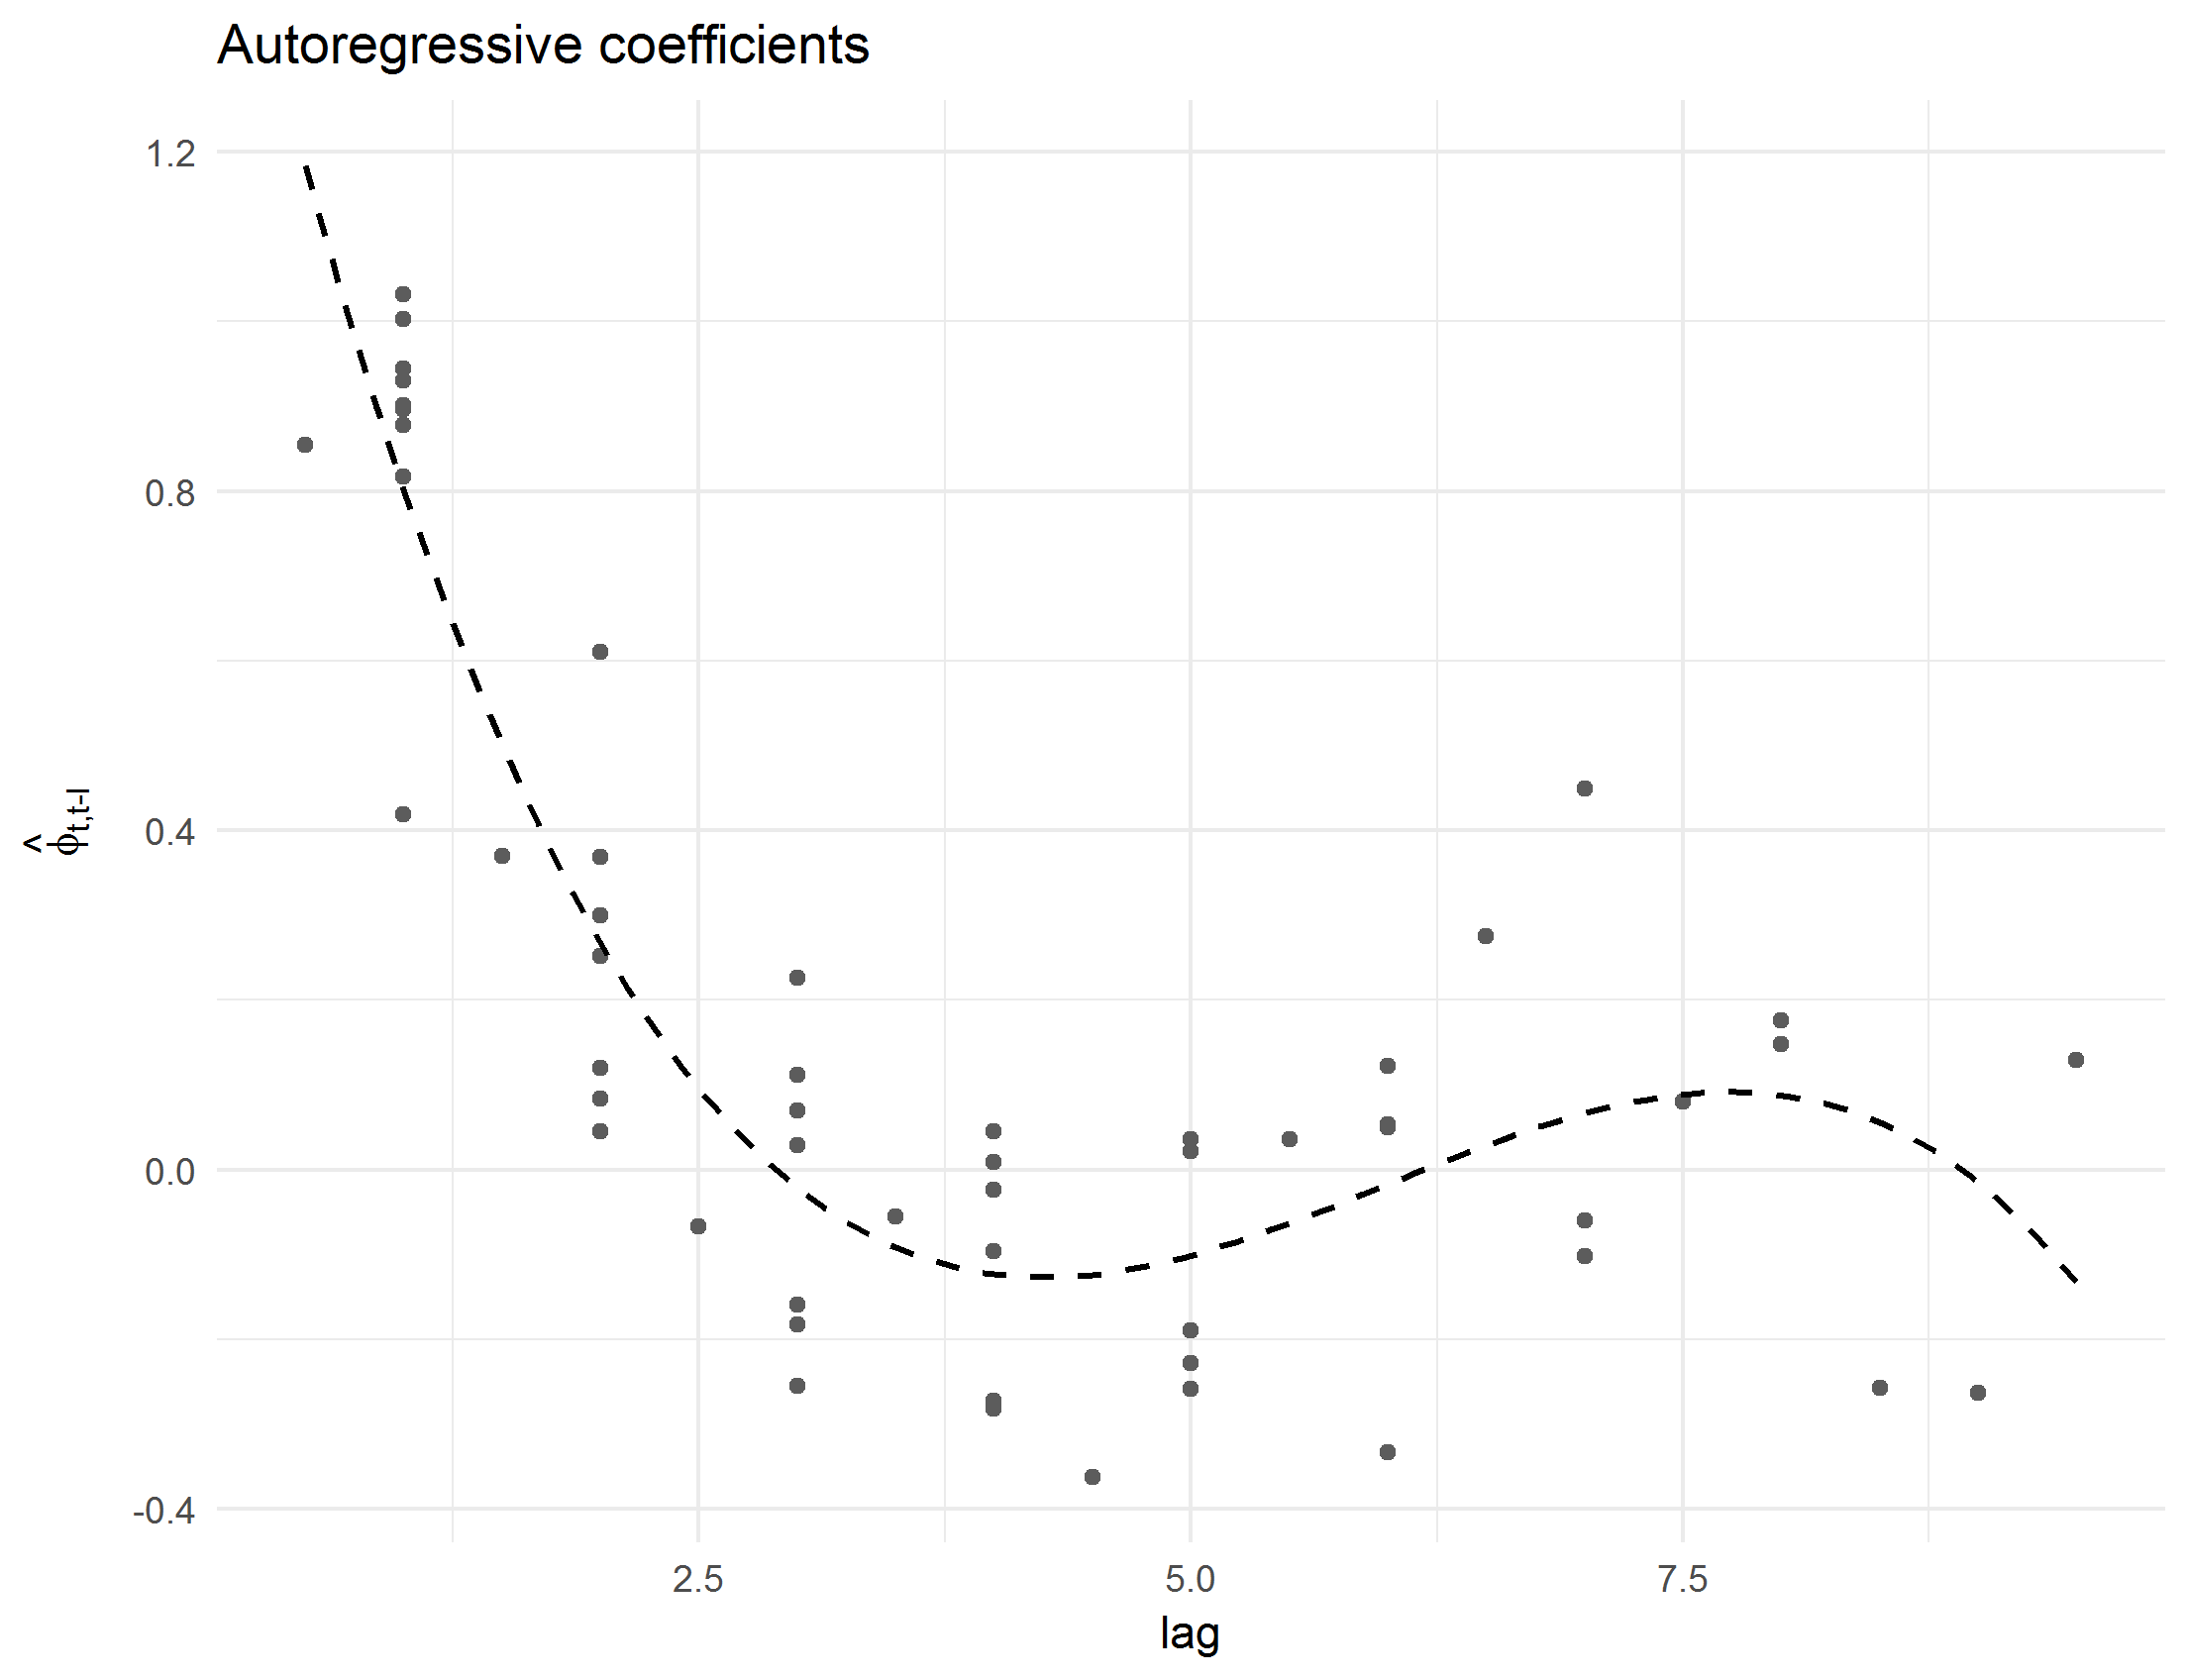
\includegraphics[width=5.5cm]{img/cattle/cattleA-regressogram-with-cubic-smooth}};
		\node[right]  at (0,7) {\footnotesize\textcolor{paleale}{Sample generalized autoregressive}};
		\node[right]  at (0,6.6) {\footnotesize\textcolor{paleale}{parameters}};
		\node[right] (phi) at (.2,1) {\footnotesize\textcolor{mint}{$\phi_{ts} = x'_{ts}\gamma$}};
		\node[right] (x_phi) at (.2,0.5) {\footnotesize\textcolor{mint}{$\phantom{\phi_{ts}} = \gamma_0 +\gamma_1 \left(t - s\right) $}};
		\node[right] (x_phi) at (.2,0) {\footnotesize\textcolor{mint}{$\phantom{\phi_{ts} = \gamma_0 }+ \gamma_2\left(t - s\right)^2 + \gamma_3 \left(t - s\right)^3$}};
		\path[<-, color=mint, line width=.7] (2.2,1.2) edge [in = 200] (4.7,3.27);
	\end{tikzpicture}
	\vspace{0pt}
\end{column}
\begin{column}[b]{5.5cm}
   \centering
\begin{tikzpicture}%[show background grid] %% Use grid for positioning, then turn off
		% \node[right] at (.5,8) {\comment{\ECFAugie(Left of this ruled out)}};
		\node[right]  at (0,4) {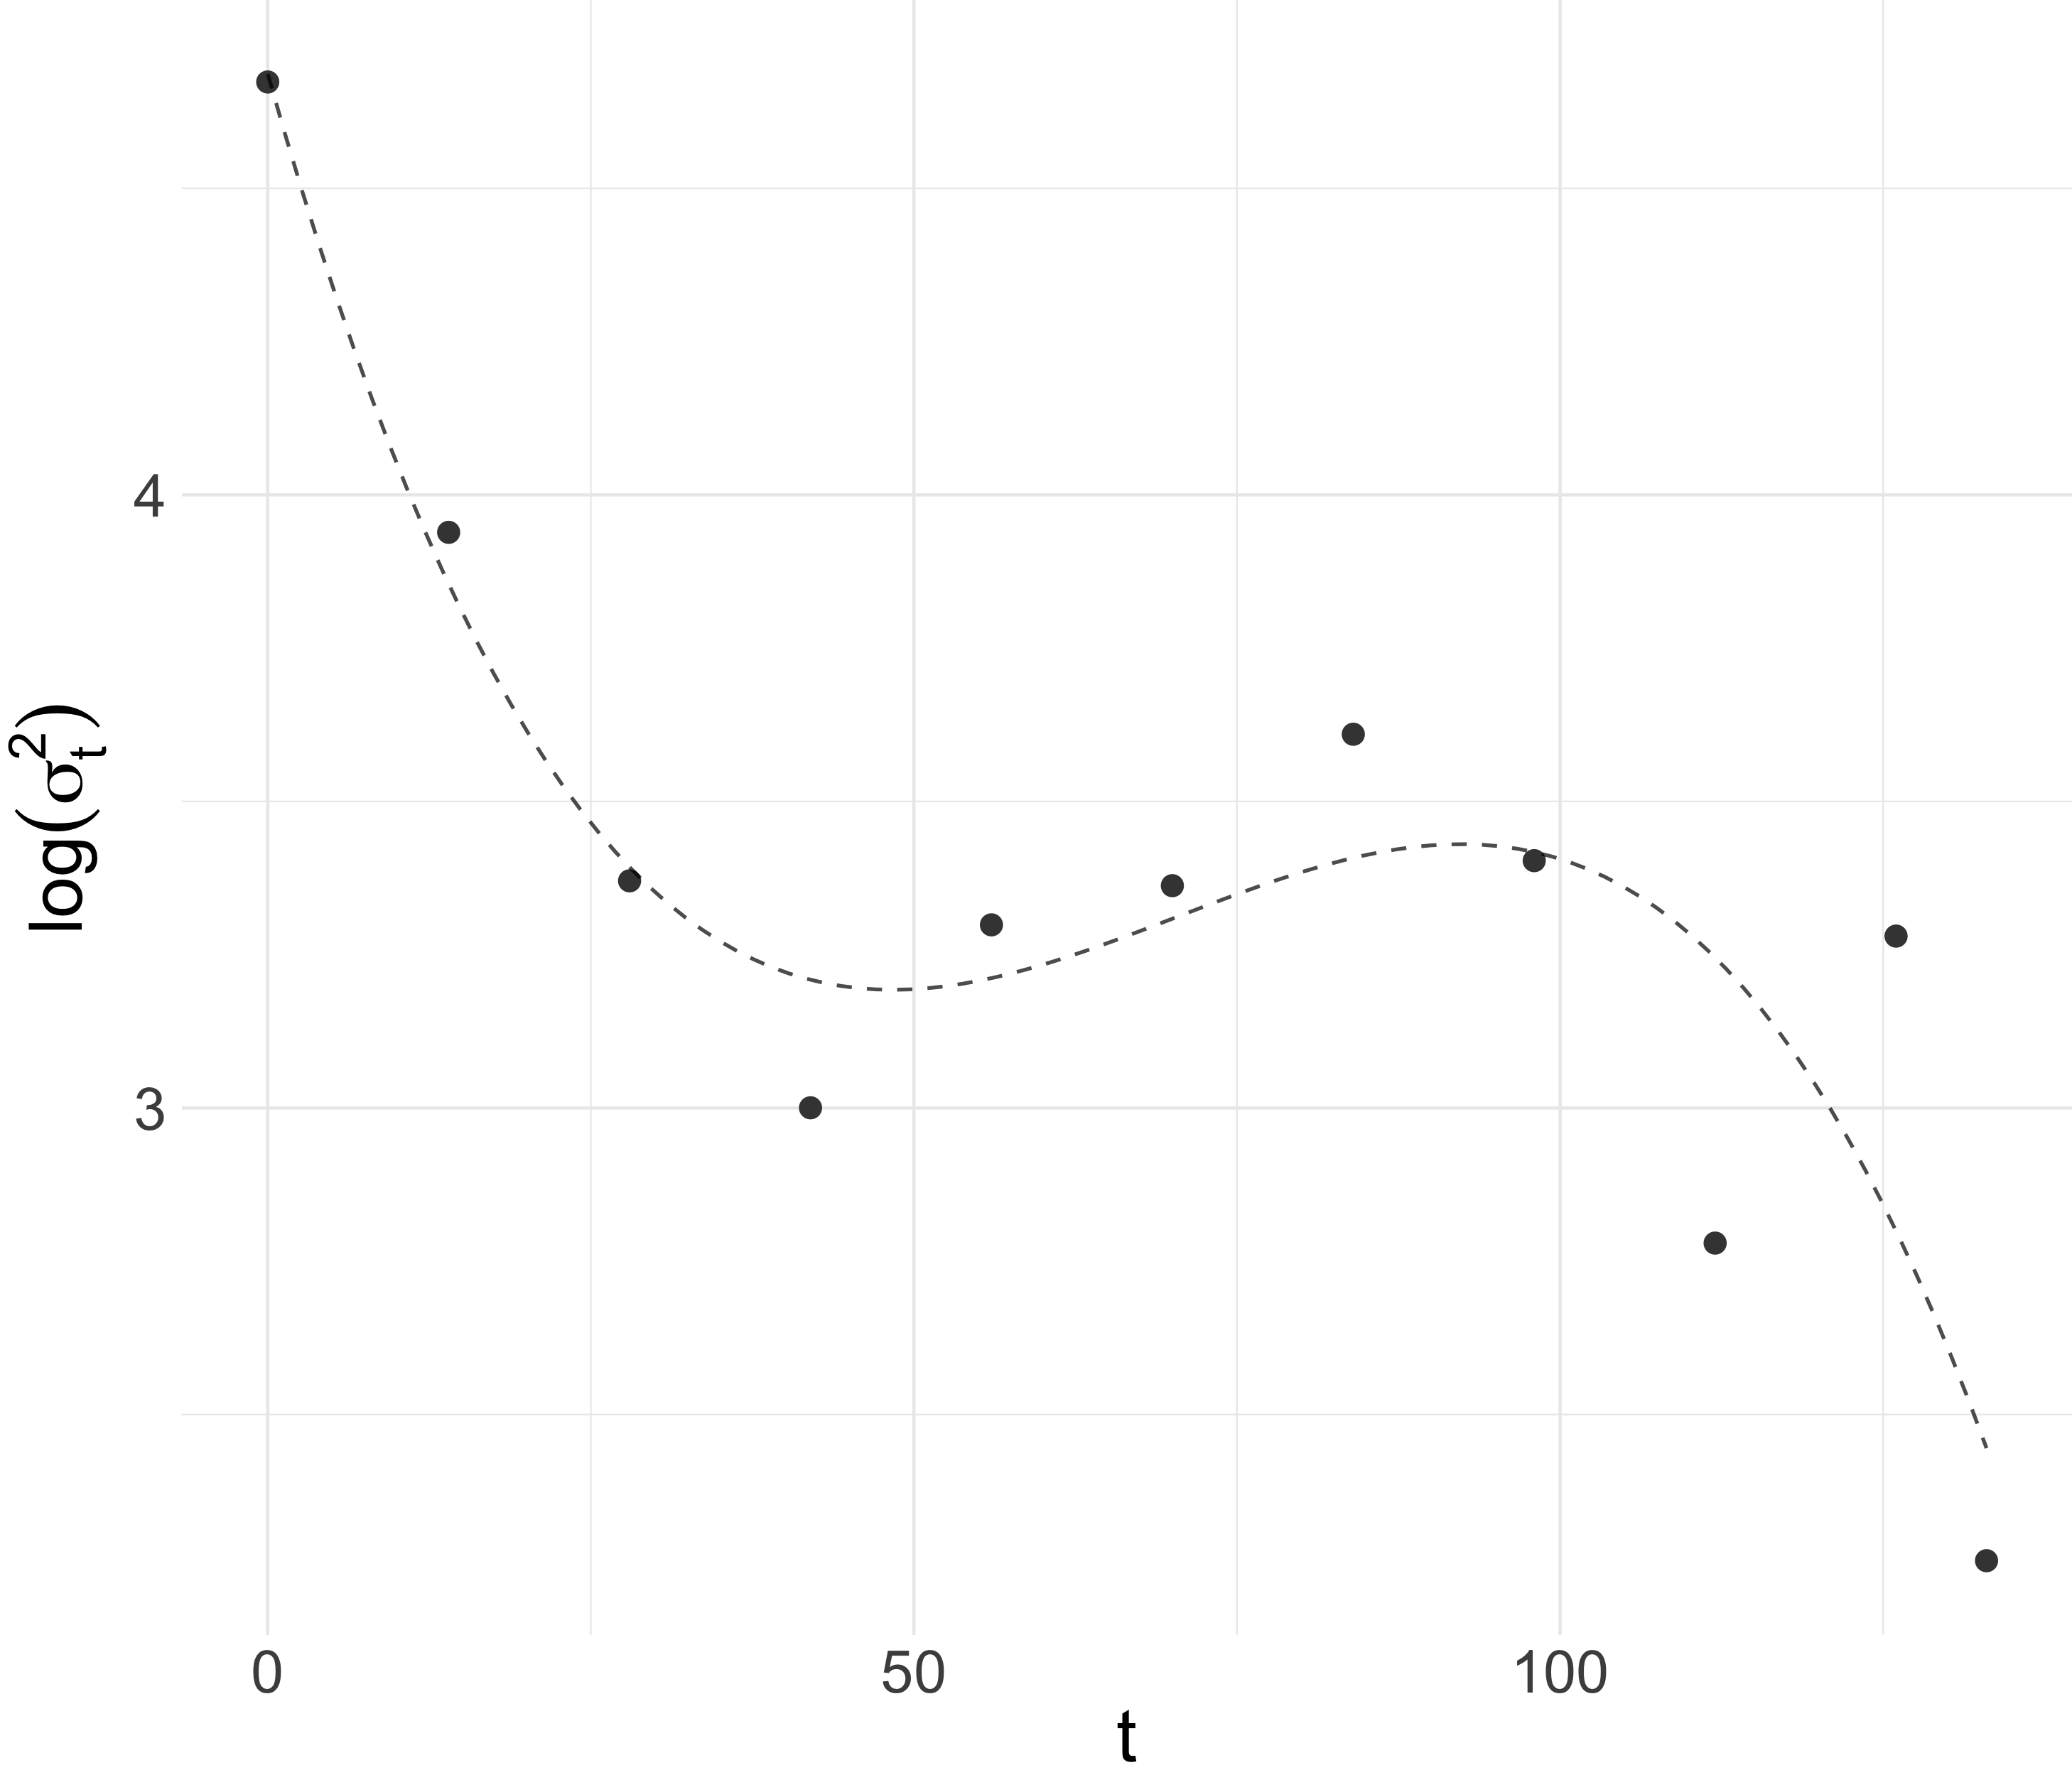
\includegraphics[width=5.5cm]{img/cattle/cattleA-innovariogram-with-cubic-smooth}};
		\node[right] at (0,6.6) {\footnotesize\textcolor{paleale}{Sample innovation variances}};
		\node[right] (sigma) at (.2,1) {\textcolor{mint}{\footnotesize$\log \sigma^2_{t} = z'_{t}\xi$}};
		\node[right] (z_sigma) at (.2,0.5) {\textcolor{mint}{\footnotesize$\phantom{\log \sigma^2_{t}} = \begin{bmatrix} \xi_0 + \xi_1t + \xi_2 t^2 + \xi_3t^3 \end{bmatrix}$}};
		\node[right] (z_sigma) at (.2,0) {\textcolor{mint}{\footnotesize$\phantom{\log \sigma^2_{t} = \begin{bmatrix} \xi_0 + \xi_1t + \xi_2 t^2 + \xi_3t^3 \end{bmatrix}}$}};
		\path[<-, color=mint, line width=.7] (2.3,1.2) edge [in = 200] (5.2,2.8);
	\end{tikzpicture}
	\vspace{0pt}
\end{column}
\end{columns}

\end{frame}


\begin{frame}{\textit{A joint mean-covariance model for the cattle weights}}
\begin{columns}
\begin{column}{6cm}
\begin{align*}
y_{ij} &= f\left(t_i  \right) + \alpha_i + \epsilon^*_{ij}, \\
 i &= 1, \dots, N=30\\ 
 j &= 1, \dots, 11,
\end{align*} 
where the $\alpha_i \stackrel{\mbox{\tiny{i.i.d.}}}{\sim} N\left(0 ,\sigma_\alpha^2\right)$ mutually independent of $ \epsilon^*_{ij} = \left( \epsilon^*_{i1},\dots, \epsilon^*_{ip_i} \right)'$,
\begin{align*}
\epsilon^*_i &\sim N\left(0, \Sigma\right),\\
f &\in \hilbert  = \mathcal{C}^2\left[\Re^+\right],
\end{align*} \footnotesize
and $J\left(f\right) = \int_0^1 \left(f''\left(x\right)\right)^2\;dx$.
\end{column}
\begin{column}{5.5cm}
\centering
\begin{tikzpicture}%[show background grid] %% Use grid for positioning, then turn off
		% \node[right] at (.5,8) {\comment{\ECFAugie(Left of this ruled out)}};
		\node[right]  at (0,3) {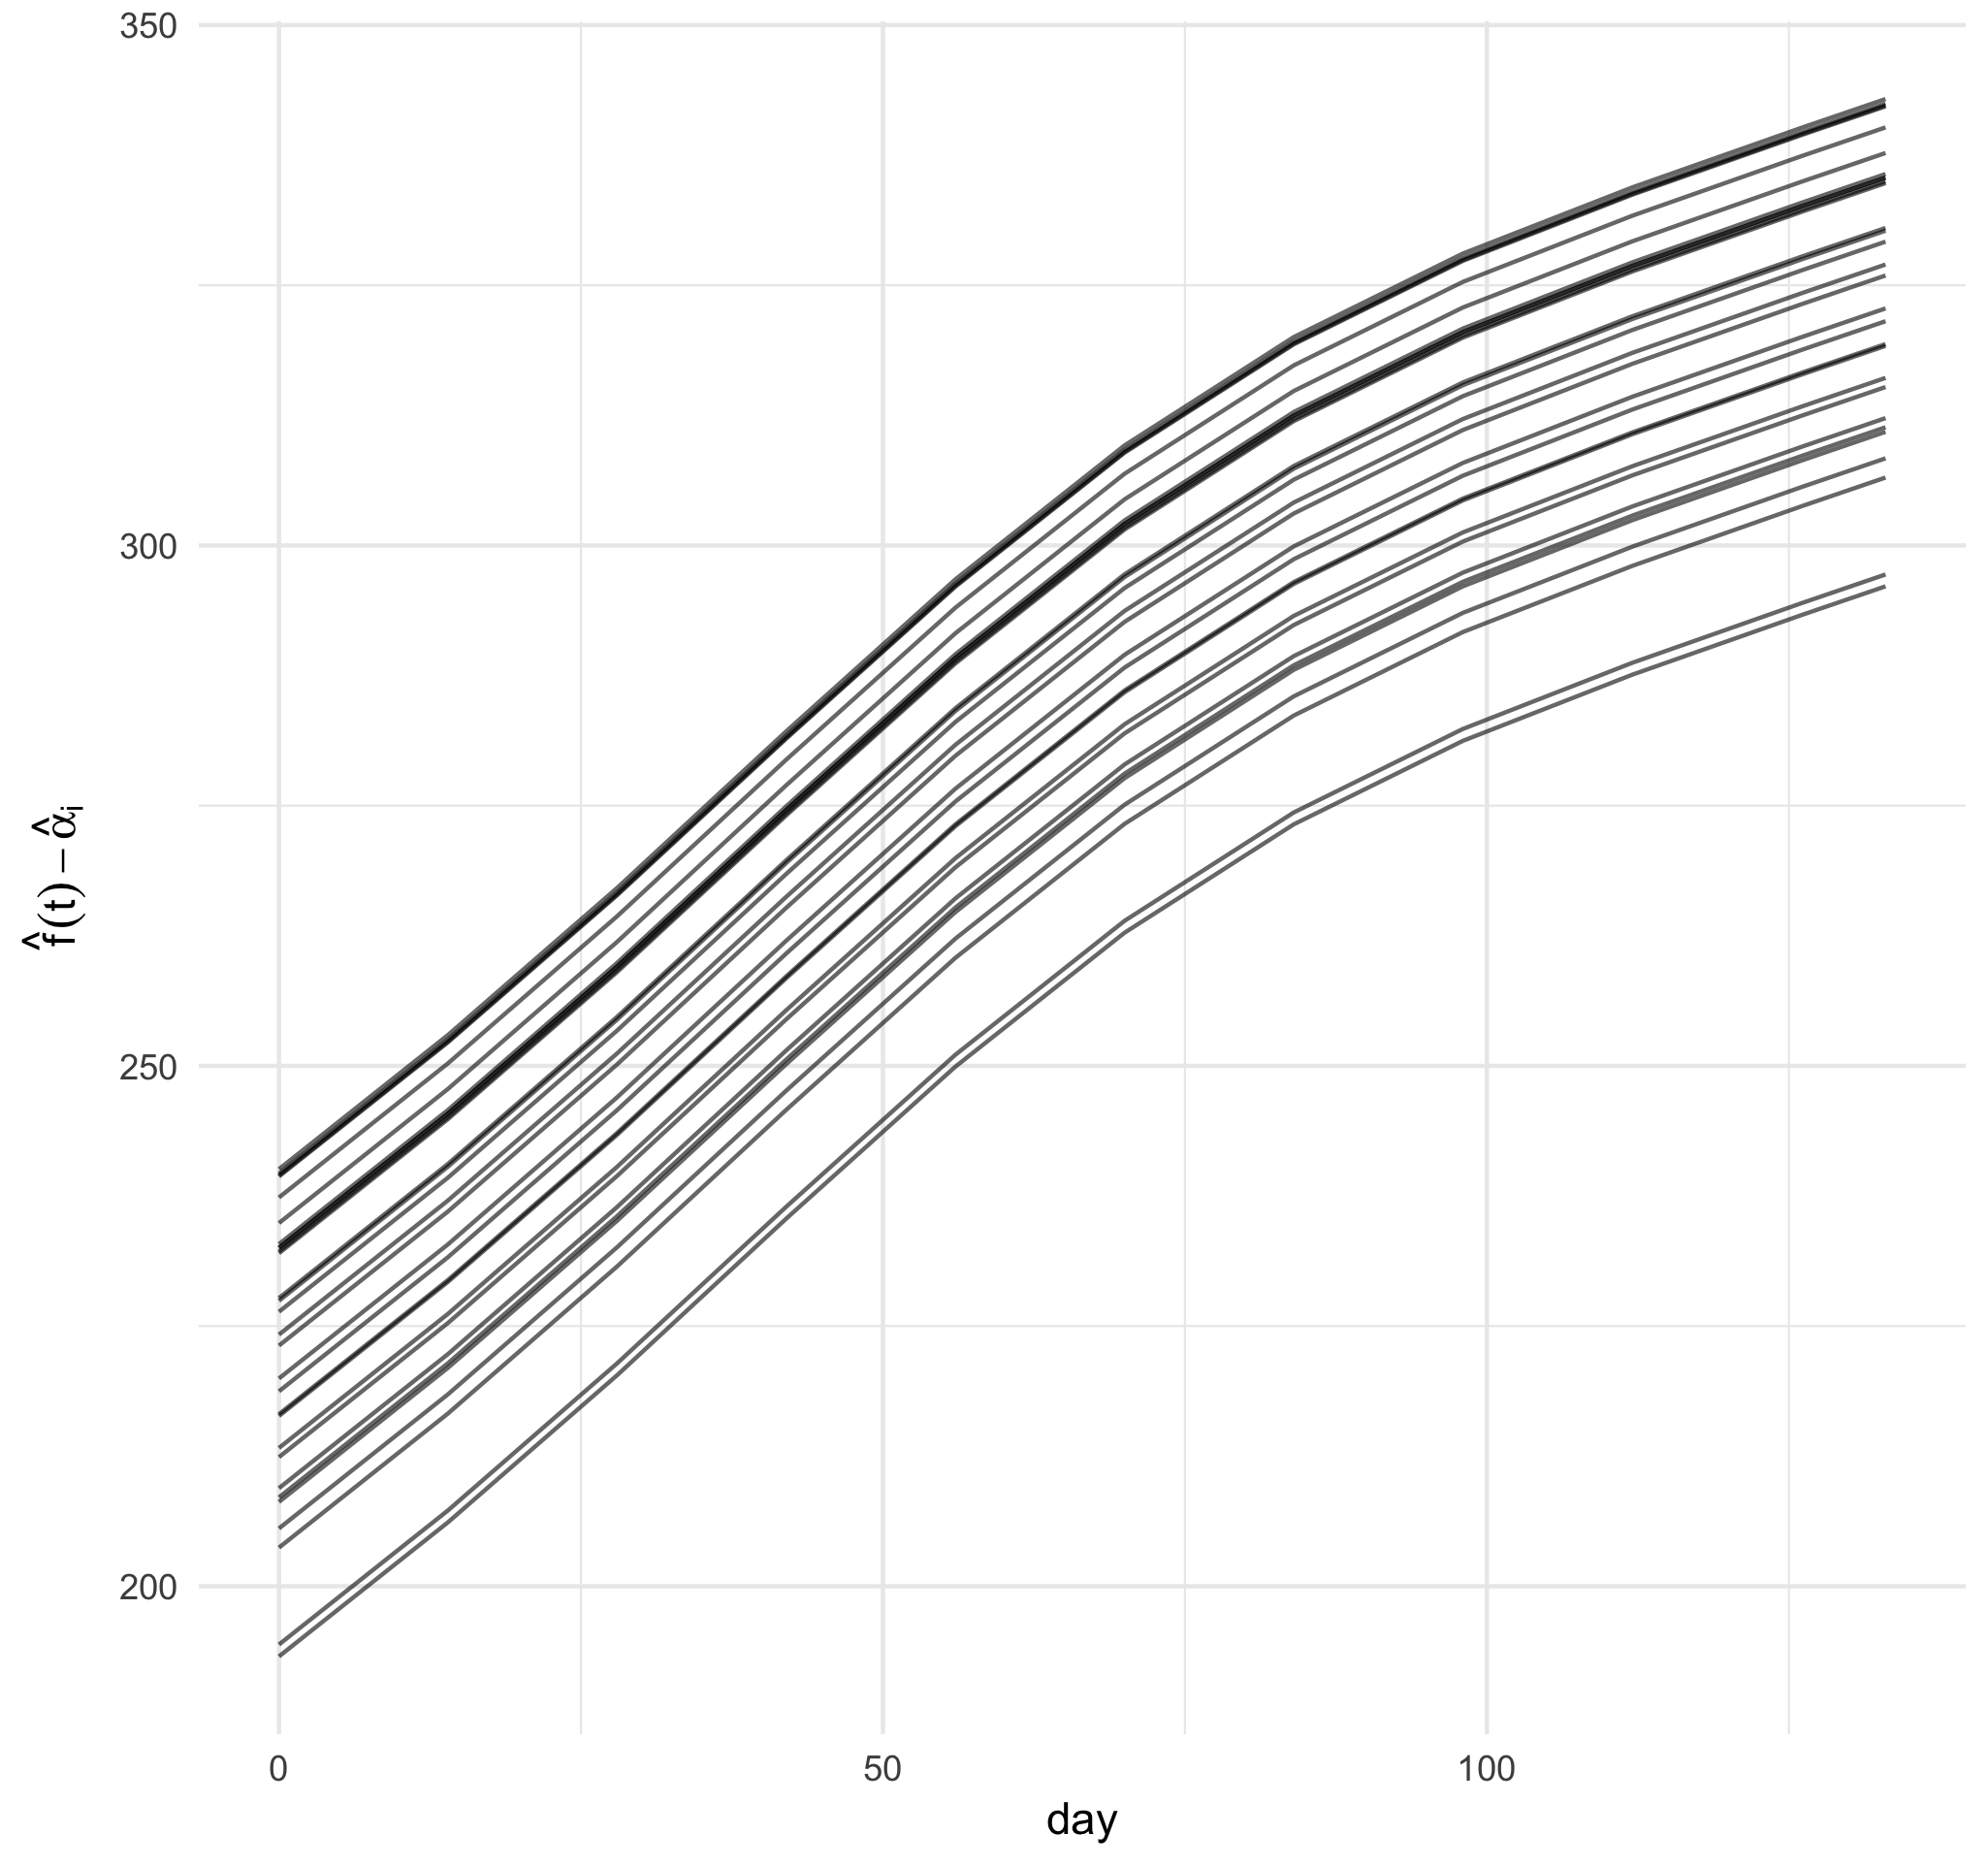
\includegraphics[width = 5.5cm]{img/cattle/cattleA-weights-vs-time-mean-fit}};
		\node[right] (mu) at (.75,4.9) {\textcolor{gray!100}{\footnotesize$\hat{\mu}_i =  \hat{f}\left(t_i  \right) + \hat{\alpha}_i$}};
	\end{tikzpicture}
\end{column}
\end{columns} 
\end{frame}


\begin{frame}{\textit{Modeling the Cholesky decomposition}}
\begin{columns}
\begin{column}[]{6cm}
\centering
\begin{figure}
  \centering
  \subfloat[\scriptsize $S$]{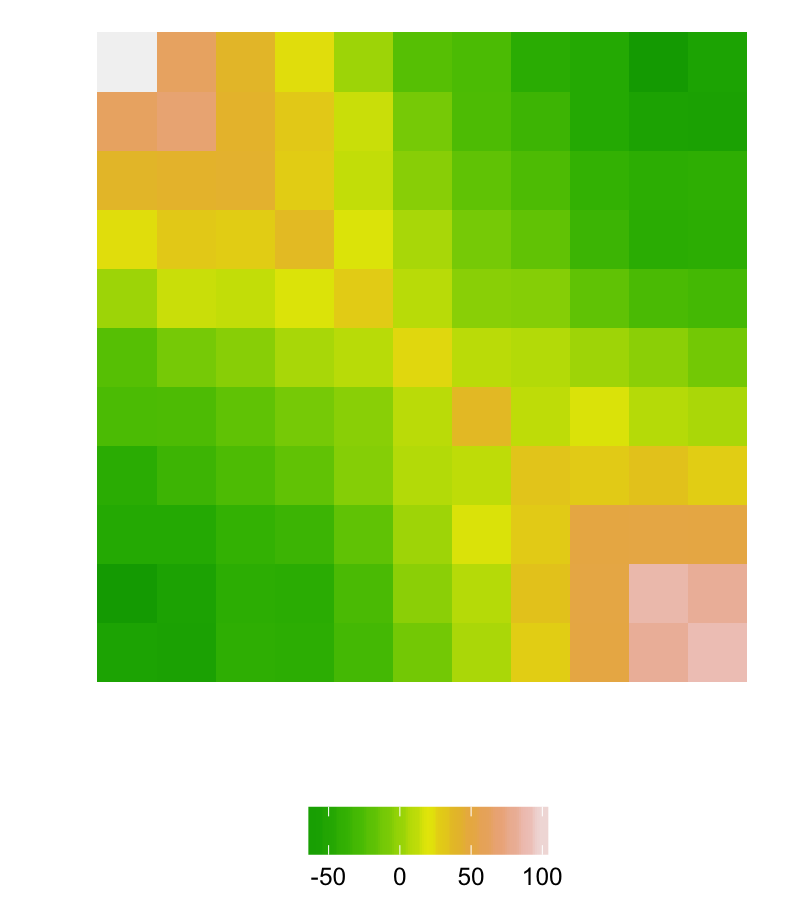
\includegraphics[height=2.9cm,width=2.9cm]{img/chapter-5/cattle-cholesky-estimate-ggplot-S}}
  \subfloat[\scriptsize$\hat{\Sigma} = {\hat{T'}}^{-1}\hat{D}{\hat{T}}^{-1}$]{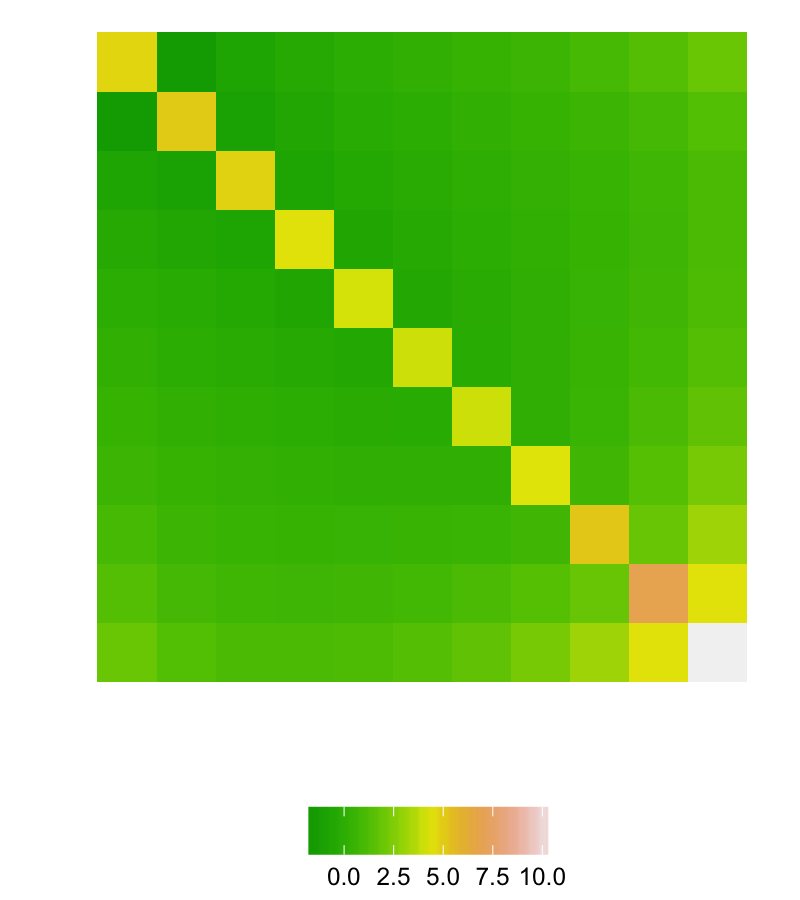
\includegraphics[height=2.9cm,width=2.9cm]{img/chapter-5/cattle-cholesky-estimate-ggplot-Sigma}}\hfill
  \subfloat[\scriptsize $\hat{\phi}\left(t,s\right)$]{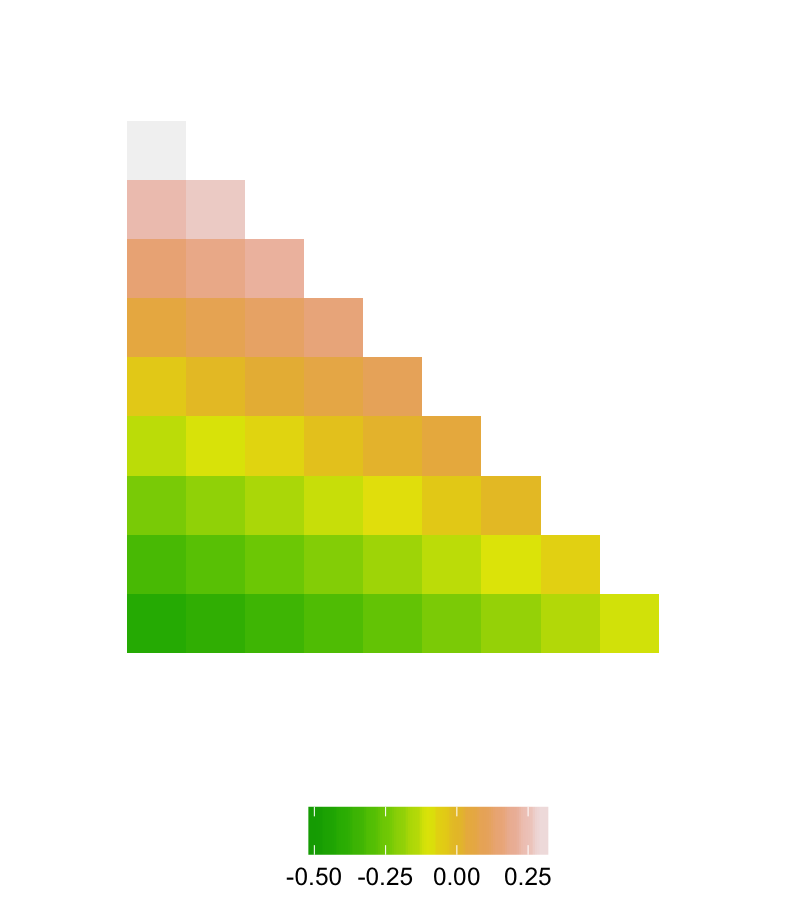
\includegraphics[height=2.9cm,width=2.9cm]{img/chapter-5/cattle-cholesky-estimate-ggplot-phi}}
  \subfloat[\scriptsize$\hat{\sigma}^2\left(t\right)$]{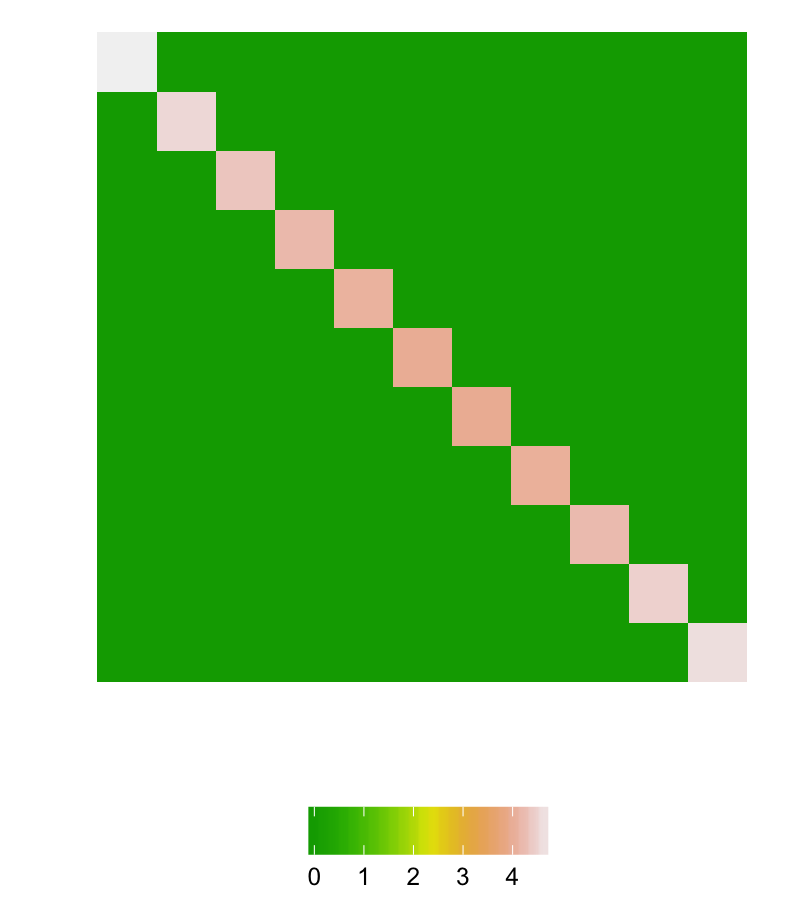
\includegraphics[height=2.9cm,width=2.9cm]{img/chapter-5/cattle-cholesky-estimate-ggplot-log-sigma2}}
\end{figure}
\end{column}
\begin{column}[]{5.5cm} \footnotesize
Model
\begin{equation*}% \label{eq:cattleA-dynamic-cond-mixed-model-1}
\epsilon^*\left(t_{ij}\right) = \sum_{k < j} \phi\left( t_{ij}, t_{ik} \right) \epsilon^*\left(t_{ij}\right) + \epsilon\left(t_{ij}\right)
\end{equation*}
where $\epsilon\left(t\right) \sim N\left(0, \sigma^2\left(t\right)\right)$ and 
\scriptsize
\begin{align*} 
\phi \in \hilbert &= \hilbert_{\left[l\right]} \otimes \hilbert_{\left[m\right]}\\
\hilbert_{\left[l\right]} = &\phantom{\oplus} \bigg\{ \phi: \ddot{\phi} = 0 \bigg\} \\
&\oplus  \left\{\phi: \phi\left(0\right),\dot{\phi}\left(0\right) = 0;\; \ddot{\phi} \in \mathcal{L}_2\left[0,1\right]   \right\} \\
\hilbert_{\left[m\right]} = &\phantom{\oplus} \bigg\{ \phi: \phi \propto 1 \bigg\} \\
&\oplus \left\{ \phi: \int_0^1 \phi \;dx = 0, \;\; \dot{\phi} \in \mathcal{L}_2\left[0,1\right]  \right\} 
\end{align*} 
\end{column}
\end{columns} 
\end{frame}


\begin{frame}{The functional components of $\phi$}{}
\centering
\begin{tikzpicture}%[show background grid] %% Use grid for positioning, then turn off
		% \node[right] at (.5,8) {\comment{\ECFAugie(Left of this ruled out)}};
		\node[right]  at (0,2) {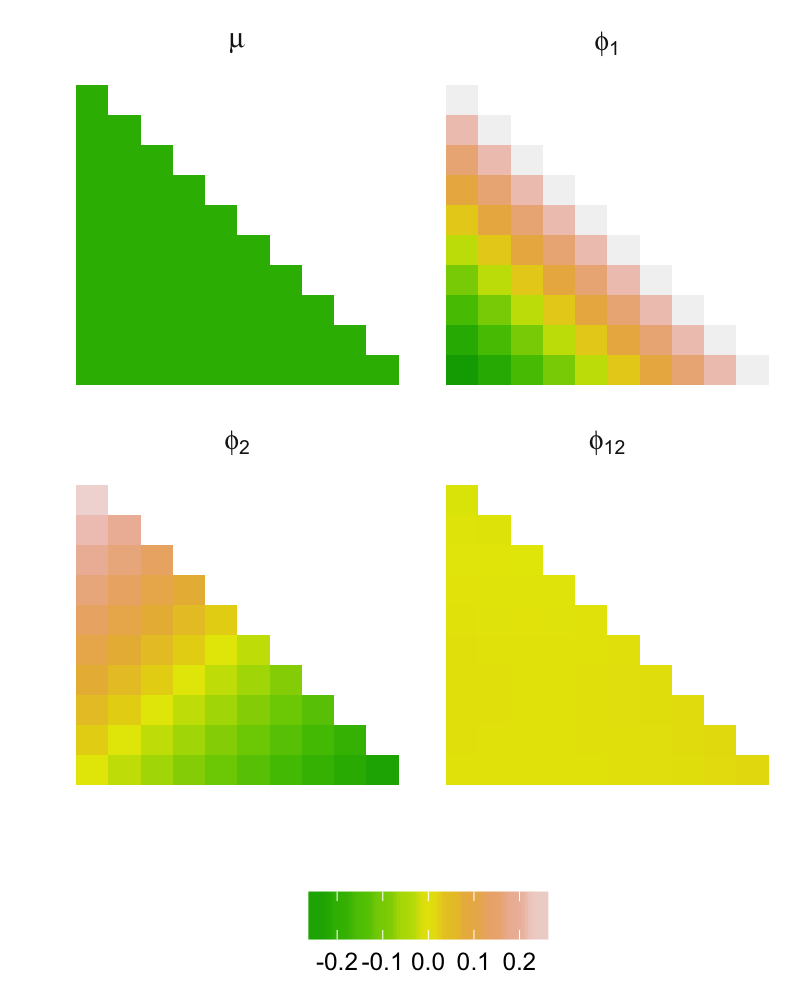
\includegraphics[width = 6cm]{img/chapter-5/cattle-ssanova-estimate-lattice} };
		\fill [white] (4.75,5.43) circle [radius=4pt];
		\node[right] (mu) at (4,5.4) {\textcolor{gray!100}{\scriptsize$\vert\vert \phi_{l} \vert \vert^2 = 1.914$}};
		\fill [white] (4.75,2.49) circle [radius=7pt];
		\fill [white] (1.81,2.49) circle [radius=7pt];
		\fill [white] (1.81,5.43) circle [radius=7pt];
		\node[right] (mu) at (4,5.4) {\textcolor{gray!100}{\scriptsize$\vert\vert \phi_{l} \vert \vert^2 = 1.914$}};
		\node[right] (mu) at (4,2.49) {\textcolor{gray!100}{\scriptsize$\vert\vert \phi_{lm} \vert \vert^2 \approx 0$}};
		\node[right] at (1,2.49) {\textcolor{gray!100}{\scriptsize$\vert\vert \phi_{m} \vert \vert^2 = 0.790$}};
		\node[right] (mu) at (1.81,5.4) {\textcolor{gray!100}{$\mu$}};
	\end{tikzpicture}
\end{frame}

%%%%%%%%%%%%%%%%%%%%%%%%%%%%%%%%%%%%%%%%%%%%%%%%%%%%%%%%%%%%%%%%%%%%%%%%%%%%
%%%%%%%%%%%%%%%%%%%%%%%%%%%%%%%%%%%%%%%%%%%%%%%%%%%%%%%%%%%%%%%%%%%%%%%%%%%%
%%%%%%%%%%%%%%%%%%%%%%%%%%%%%%%%%%%%%%%%%%%%%%%%%%%%%%%%%%%%%%%%%%%%%%%%%%%%
%%%%%%%%%%%%%%%%%%%%%%%%%%%%%%%%%%%%%%%%%%%%%%%%%%%%%%%%%%%%%%%%%%%%%%%%%%%%


\begin{frame}[c]{\textit{Concluding Remarks and Future Work}}

\end{frame}


\begin{frame}[c]{\textit{Thank you!}}

\end{frame}

%%%%%%%%%%%%%%%%%%%%%%%%%%%%%%%%%%%%%%%%%%%%%%%%%%%%%%%%%%%%%%%%%%%%%%%%%%%%
%%%%%%%%%%%%%%%%%%%%%%%%%%%%%%%%%%%%%%%%%%%%%%%%%%%%%%%%%%%%%%%%%%%%%%%%%%%%
%%%%%%%%%%%%%%%%%%%%%%%%%%%%%%%%%%%%%%%%%%%%%%%%%%%%%%%%%%%%%%%%%%%%%%%%%%%%
%%%%%%%%%%%%%%%%%%%%%%%%%%%%%%%%%%%%%%%%%%%%%%%%%%%%%%%%%%%%%%%%%%%%%%%%%%%%

\begin{frame}[allowframebreaks] %allow to expand references to multiple frames (slides)

\frametitle{References}
%\bibliography{Master} %bibtex file name without .bib extension

\end{frame}



%%%%%%%%%%%%%%%%%%%%%%%%%%%%%%%%%%%%%%%%%%%%%%%%%%%%%%%%%%%%%%%%%%%%%%%%%%%%
%%%%%%%%%%%%%%%%%%%%%%%%%%%%%%%%%%%%%%%%%%%%%%%%%%%%%%%%%%%%%%%%%%%%%%%%%%%%
%%%%%%%%%%%%%%%%%%%%%%%%%%%%%%%%%%%%%%%%%%%%%%%%%%%%%%%%%%%%%%%%%%%%%%%%%%%%
%%%%%%%%%%%%%%%%%%%%%%%%%%%%%%%%%%%%%%%%%%%%%%%%%%%%%%%%%%%%%%%%%%%%%%%%%%%%

\begin{frame}[c]{\textit{Appendix}}

\end{frame}




%\begin{frame}[c]{\textit{Incoherence of the GARPs: a simple example}}{}
%\footnotesize{
%\begin{align*}
%y_{it} &= t^{th}\mbox{ measurement on subject } i \\
%&=\left\{ \begin{array}{ll} \epsilon_{it}, & t = 1, \\
%	\phi y_{i,t-1} + \epsilon_{it}, &  t = 2,3,4, \end{array} \right. \;\; \epsilon_i = \left(\epsilon_{i1}, \dots, \epsilon_{ip_i} \right)'\sim N\left(0, I\right)
%\end{align*}
%
%For a subject with a complete set of observations, $D = I_4$,} 
%\scriptsize
%\begin{equation*}
%T = \begin{bmatrix}
%1& 0 & 0 & 0  \\
%\phi & 1& 0 & 0 \\
%0 & \phi & 1& 0 \\
%0 & 0 & \phi & 1\\
%\end{bmatrix}, 
%\Sigma = \begin{bmatrix} 
%1 & \phi & \phi^2 & \phi^3 \\
%\phi & 1 + \phi^2  & \phi^2 + \phi^3 &  \phi^3 + \phi^4 \\
%\phi^2 & \phi^2 + \phi^3 & 1 + \phi^2 + \phi^4 & \phi + \phi^3 + \phi^5 \\
%\phi^3 & \phi^3 + \phi^4 & \phi + \phi^3 + \phi^5 & 1 + \phi^2 + \phi^4 + \phi^6 
%\end{bmatrix}
%\end{equation*}
%
%\footnotesize{
%\begin{center}
%\begin{tabular}{llll}
%\hline
%\\
%Subject 1 & $Y_1 = \left( y_{11}, y_{12}, y_{13} \right)$ & $t_1 = \left(1, 2, 4\right)'$ & $D_1 = T'_1\Sigma_1 T_1$ \\
%Subject 2 & $Y_2 = \left( y_{21}, y_{22}, y_{23} \right)$ & $t_2 = \left(1, 3, 4\right)'$ & $D_2 = T'_2\Sigma_2 T_2$\\
%\end{tabular}
%\end{center}}
%
%\scriptsize{
%\begin{align*}
%T_1 &= \begin{bmatrix}
%1& 0 & 0  \\
%-\phi & 1& 0  \\
%0 & -\phi^2 & 1
%\end{bmatrix}, \;\;
%D_1 = \begin{bmatrix} 
%1 & 0 & 0  \\
%0 & 1 & 0 \\
%0 & 0 & 1 + \phi^2
%\end{bmatrix}, \\
%T_2 &= \begin{bmatrix}
%1& 0 & 0  \\
%-\phi^2 & 1& 0  \\
%0 & -\phi & 1
%\end{bmatrix}, \;\;
%D_2 = \begin{bmatrix} 
%1 & 0 & 0  \\
%0 & 1 + \phi^2 & 0 \\
%0 & 0 & 1 
%\end{bmatrix}
%\end{align*}}
%
%\end{frame}
%


\begin{frame}[c]{\emph{Tensor Product Cubic Spline Space}}{\textit{Reproducing Kernels}}

\scriptsize
\begin{tabular}{lll} % centered columns (4 columns)
\hline 
\hline %inserts double horizontal lines
Subspace 	& 		Reproducing kernel 		 \\
\hline % inserts single horizontal line
$\hilbert_{00\left[1\right]} \otimes \hilbert_{00\left[2\right]}$ & 	$1$	\\ [1ex] 
$\hilbert_{01\left[1\right]} \otimes \hilbert_{00\left[2\right]} $& 	$k_1\left(x_1\right)k_1\left(y_1\right)$	\\ [1ex] 
$\hilbert_{00\left[1\right]} \otimes \hilbert_{01\left[2\right]} $& 	$k_1\left(x_2\right)k_1\left(y_2\right)$	\\ [1ex] 
$\hilbert_{01\left[1\right]} \otimes \hilbert_{01\left[2\right]}$ & 	$k_1\left(x_1\right)k_1\left(y_1\right)k_1\left(x_2\right)k_1\left(y_2\right)$ \\ [1ex] 
$\hilbert_{1\left[1\right]} \otimes \hilbert_{00\left[2\right]}$  	& 	$k_2\left(x_1\right)k_2\left(y_1\right) - k_4\left(x_1 - y_1\right)$	\\ [1ex] 
$\hilbert_{00\left[1\right]} \otimes \hilbert_{1\left[2\right]}$  	& 	$k_2\left(x_2\right)k_2\left(y_2\right) - k_4\left(x_2 - y_2\right)$	\\ [1ex] 
$\hilbert_{1\left[1\right]} \otimes \hilbert_{01\left[2\right]}$ 	& 	$\left[k_2\left(x_1\right)k_2\left(y_1\right) - k_4\left(x_1 - y_1\right)\right]k_1\left(x_2\right)k_1\left(y_2\right)$ \\ [1ex]  
$ \hilbert_{01\left[1\right]}\otimes  \hilbert_{1\left[2\right]}$ 	& 	$k_1\left(x_1\right)k_1\left(y_1\right)\left[k_2\left(x_2\right)k_2\left(y_2\right) - k_4\left(x_2 - y_2\right)\right]$ \\ [1ex]  
$\hilbert_{1\left[1\right]} \otimes \hilbert_{1\left[2\right]}$  & $\left[k_2\left(x_1\right)k_2\left(y_1\right) - k_4\left(x_1 - y_1\right)\right]\left[k_2\left(x_2\right)k_2\left(y_2\right) - k_4\left(x_2 - y_2\right)\right]$	\\ [1ex]  
\hline %inserts single line
\hline %inserts single line
\end{tabular}
\end{frame}


\begin{frame}{\textit{A General Form for Multiple-Term RK Hilbert Spaces}}{}

\end{frame}


\begin{frame}{\textit{Obtaining the solution}  $\phi_\lambda$}{When $\tildeK_{_{V}}$ is not full rank}
\footnotesize
\begin{equation} \label{eq:normal-equation-cholesky}
\begin{bmatrix}
\tildeB'\tildeB & \tildeB'\tildeK_{_{ V}} \\
\tildeK_{_{ V}}'\tildeB & \tildeK_{_{ V}}'\tildeK_{_{ V}} + \lambda K_{_{ V}}\\
\end{bmatrix}
= \begin{bmatrix}
C'_1 & 0 \\
C'_2  & C'_3 
\end{bmatrix}
\begin{bmatrix}
C_1 & C_2 \\
0  & C_3 
\end{bmatrix}
\end{equation}
\noindent
where $\tildeB'\tildeB = C'_1 C_1$, $C_2 = \left(C'_1\right)^{-1} \tildeB' \tildeK_{_{ V}}$, and $C'_3 C_3 = \lambda K_{_{ V}} +  \tildeK_{_{ V}}'\left( I - \tildeB\left( \tildeB' \tildeB \right)^{-1} \tildeB' \right)\tildeK_{_{ V}}$. Using an exchange of indices known as pivoting, one may write 
\begin{equation*}
C_3 = \begin{bmatrix} H_1 & H_2 \\ 0 & 0 \end{bmatrix} = \begin{bmatrix} H \\  0 \end{bmatrix},
\end{equation*}
\noindent
where $H_1$ is nonsingular. Define
\begin{equation} \label{eq:cholesky-factor-mod}
\tilde{C}_3 = \begin{bmatrix}
H_1 & H_2 \\
0  & \delta I 
\end{bmatrix}, \;\;
\tilde{C} = \begin{bmatrix}
C_1 & C_2 \\
0  & \tilde{C}_3 
\end{bmatrix};
\end{equation}
\end{frame}


\begin{frame}{\textit{Obtaining the solution}  $\phi_\lambda$}{When $\tildeK_{_{V}}$ is not full rank}
\footnotesize
\begin{equation} \label{eq:normal-equation-cholesky}
\begin{bmatrix}
\tildeB'\tildeB & \tildeB'\tildeK_{_{ V}} \\
\tildeK_{_{ V}}'\tildeB & \tildeK_{_{ V}}'\tildeK_{_{ V}} + \lambda K_{_{ V}}\\
\end{bmatrix}
= \begin{bmatrix}
C'_1 & 0 \\
C'_2  & C'_3 
\end{bmatrix}
\begin{bmatrix}
C_1 & C_2 \\
0  & C_3 
\end{bmatrix}
\end{equation}
\noindent
where $\tildeB'\tildeB = C'_1 C_1$, $C_2 = \left(C'_1\right)^{-1} \tildeB' \tildeK_{_{ V}}$, and $C'_3 C_3 = \lambda K_{_{ V}} +  \tildeK_{_{ V}}'\left( I - \tildeB\left( \tildeB' \tildeB \right)^{-1} \tildeB' \right)\tildeK_{_{ V}}$. Using an exchange of indices known as pivoting, one may write 
\begin{equation*}
C_3 = \begin{bmatrix} H_1 & H_2 \\ 0 & 0 \end{bmatrix} = \begin{bmatrix} H \\  0 \end{bmatrix},
\end{equation*}
\noindent
where $H_1$ is nonsingular. Define
\begin{equation} \label{eq:cholesky-factor-mod}
\tilde{C}_3 = \begin{bmatrix}
H_1 & H_2 \\
0  & \delta I 
\end{bmatrix}, \;\;
\tilde{C} = \begin{bmatrix}
C_1 & C_2 \\
0  & \tilde{C}_3 
\end{bmatrix};
\end{equation}
\end{frame}

\begin{frame}{\textit{Obtaining the solution}  $\phi_\lambda$}{When $\tildeK_{_{V}}$ is not full rank}
\footnotesize

Then
\begin{equation} \label{eq:cholesky-factor-mod-inverse}
\tilde{C}^{-1} = \begin{bmatrix}
C_1^{-1} & -C_1^{-1} C_2 \tilde{C}_3^{-1} \\
0  & \tilde{C}_3^{-1}
\end{bmatrix}.
\end{equation}

Premultiplying \eqref{eq:normal-equation-cholesky} by $(\tilde{C}')^{-1}$, 
\begin{equation*}% \label{eq:vectorized-normal-equations-cholesky}
\begin{bmatrix}
I & 0 \\
0 & (\tilde{C}'_3)^{-1} C'_3 C_3 \tilde{C}_3^{-1}\\
\end{bmatrix}
\begin{bmatrix}
\tilde{d}\\
\tilde{c}\\
\end{bmatrix}
= \begin{bmatrix}
(C'_1)^{-1} \tildeB'\tildeY \\
(\tilde{C}'_3)^{-1} \tildeK_{_{ V}}'\left( I - \tildeB\left( \tildeB' \tildeB \right)^{-1} \tildeB' \right) \tildeY\\
\end{bmatrix}
\end{equation*}
%where $\left( \tilde{d}'\;\;\tilde{c}' \right)' =  \tilde{C}' \left( d\;\;c \right)'$. Partition $\tilde{C}_3 = \begin{bmatrix} F &  L\end{bmatrix}$; then $HF = I$ and $HL = 0$, 
%\begin{align*}
%(\tilde{C}'_3)^{-1} C'_3 C_3 \tilde{C}_3^{-1} &= \begin{bmatrix} F' \\ L' \end{bmatrix} C'_3C_3 \begin{bmatrix} F &  L\end{bmatrix} \\
%&= \begin{bmatrix} F' \\ L' \end{bmatrix} H'H \begin{bmatrix} F &  L\end{bmatrix} \\
%&= \begin{bmatrix} I & 0 \\ 0 & 0 \end{bmatrix}.
%\end{align*}
%If $L'C'_3 C_3 L = 0$, then $L'\tildeK_{_{ V}}'\left( I - \tildeB\left( \tildeB' \tildeB \right)^{-1} \tildeB' \right)\tildeK_{_{ V}} L = 0$, so $L'\tildeK_{_{ V}}'\left( I - \tildeB\left( \tildeB' \tildeB \right)^{-1} \tildeB' \right) \tildeY = 0$.
\end{frame}

\begin{frame}{\textit{Minimizing $U$, $V_{loso}$ with Multiple Smoothing Parameters}}{}

\end{frame}


\begin{frame}{\textit{A RKHS Framework for $\log \sigma^2$}}
\begin{align}  \label{eq:penalized-likelihood-functional}
%\begin{split}
L\left( \eta \right) &= \sum_{i = 1}^N \sum_{j = 1}^{p_i} \eta\left(t_{ij}\right)  + \sum_{i = 1}^N \sum_{j = 1}^{p_i} z_{ij} e^{-\eta\left(t_{ij}\right)} 
%\end{split}
\end{align}
\noindent
is continuous and convex in $\eta \in \hilbert$. We assume that the $\vert V \vert \times \mathcal{N}_0$ matrix $B$ which has $\left(i,j\right)$ element $\nu_j\left(t_i\right)$ is full column rank, so that $L\left(\eta \right)$ is strictly convex in $\hilbert$ and the minimizer of \eqref{eq:penalized-joint-loglik-given-phi} uniquely exists.  

Letting $\tilde{u}_{ij} = -z_{ij}e^{-\tilde{\eta}_{ij}}$, the Newton iteration uses the minimizer of the penalized weighted sums of squares
\begin{equation} \label{eq:penalized-weighted-sums-of-squares}
\sum_{i=1}^N\sum_{j=1}^{p_i} \left(\tilde{z}_{ij} - \eta\left(t_{ij}\right)  \right)^2 + \lambda J\left(\eta\right)
\end{equation}
\noindent
to update $\tilde{\eta}$, where $\tilde{z}_{ij} = \tilde{\eta}\left(t_{ij}\right) - \tilde{u}_{ij}$.


\end{frame}


\begin{frame}[c]{Columns}{Sometimes it's useful to split the screen}
	Test why is it gray?
	
	\begin{columns}[t]
	\begin{column}[T]{5cm}
		Here's a column where I can write a bunch of things. \\
		\comment{There are all sorts of things I can do in paragraph form.}
		
		\vspace{1em}
		\begin{block}{Blocks}
			...work in here too.
		\end{block}
	\end{column}
	\begin{column}[T]{5cm}
		\begin{itemize}
			\item Here's a column
			\item where I can itemize
			\item a bunch of things.
		\end{itemize}
	\end{column}
	\end{columns}
	
\end{frame}


\begin{frame}[c]{More Feynman diagrams}{'t Hooft operator}
	
	% \usebeamercolor[fg]{alerted text}
	\begin{center}
		\begin{tikzpicture}[line width=1.5 pt, scale=2.5]
			\draw[fermionbar] (0:.75) -- (25:.29);
			\draw[fermionnoarrow] (0:.75) -- (-25:.29);
			\draw[scalar] (0:.75) -- (0:1.25);
			\begin{scope}[shift={(1.25,0)}]
				\draw (125:.1) -- (-55:.1);
				\draw (55:.1) -- (-125:.1);			
			\end{scope}
			\draw[fermionbar] (60:.75) -- (85:.29);
			\draw[fermionnoarrow] (60:.75) -- (35:.29);
			\draw[scalar] (60:.75) -- (60:1.25);
			\begin{scope}[shift={(60:1.25)}, rotate=60]
				\draw (125:.1) -- (-55:.1);
				\draw (55:.1) -- (-125:.1);			
			\end{scope}
			\draw[fermionbar] (120:.75) -- (145:.29);
			\draw[fermionnoarrow] (120:.75) -- (95:.29);
			\draw[scalar] (120:.75) -- (120:1.25);
			\begin{scope}[shift={(120:1.25)}, rotate=120]
				\draw (125:.1) -- (-55:.1);
				\draw (55:.1) -- (-125:.1);			
			\end{scope}
			\draw[fermionbar] (300:.75) -- (325:.29);
			\draw[fermionnoarrow] (300:.75) -- (275:.29);
			\draw[scalar] (300:.75) -- (300:1.25);
			\begin{scope}[shift={(300:1.25)}, rotate=300]
				\draw (125:.1) -- (-55:.1);
				\draw (55:.1) -- (-125:.1);			
			\end{scope}
			\draw (0,0) circle (.3cm);
			% \draw[fill] (325:1) circle (.01);
			% \draw[fill] (330:1) circle (.01);
			% \draw[fill] (335:1) circle (.01);
			% \draw[fill] (340:1) circle (.01);
			% \draw[fill] (80:1) circle (.01);
			% \draw[fill] (85:1) circle (.01);
			% \draw[fill] (90:1) circle (.01);
			% \draw[fill] (95:1) circle (.01);
			% \draw[fill] (100:1) circle (.01);
			% \draw[fill] (0,0) circle (.3cm);
			% \draw[fill=white] (0,0) circle (.29cm);
			\begin{scope}
		    	\clip (0,0) circle (.3cm);
		    	\foreach \x in {-.9,-.8,...,.3}
					\draw[line width=1 pt] (\x,-.3) -- (\x+.6,.3);
		  	\end{scope}
			% \node at (0,0) {I};
			\node at (278:.6) {$\lambda$};
			\node at (323:.6) {$Q$};
			\node at (98:.6) {$\lambda$};
			\node at (143:.6) {$\overline Q$};
			\node at (290:1) {$\tilde Q$};
			\node at (130:1) {$\tilde Q$};
			\node at (300:1.5) {$v$};
			\node at (120:1.5) {$v$};
			\node at (60:1.5) {$v$};
			\node at (0:1.5) {$v$};
			\draw[fermionnoarrow] (180:.75) -- (180:.29);
			\draw[fermionnoarrow] (240:.75) -- (240:.29);
			\draw[fermion] (160:1) -- (180:.75);
			\draw[scalar] (180:.75) -- (200:1);
			\begin{scope}[shift={(200:1)}, rotate=60]
				\draw (125:.1) -- (-55:.1);
				\draw (55:.1) -- (-125:.1);			
			\end{scope}
			\draw[fermion] (260:1) -- (240:.75);
			\draw[scalar] (240:.75) -- (220:1);
			\begin{scope}[shift={(220:1)}]
				\draw (125:.1) -- (-55:.1);
				\draw (55:.1) -- (-125:.1);			
			\end{scope}
			\node at (200:1.25) {$v$};
			\node at (220:1.25) {$v$};
			\node at (265:1.2) {$Q$};
			\node at (155:1.2) {$\overline Q$};
		 \end{tikzpicture}
	\end{center}
	\usebeamercolor[fg]{normal text} 
	% Don't forget to include this when you're done futzing with colors
\end{frame}



\begin{frame}[c]{Drawing arrows onto a plot}

	\begin{tikzpicture}%[show background grid] %% Use grid for positioning, then turn off
		% \node[right] at (.5,8) {\comment{\ECFAugie(Left of this ruled out)}};
		\node[right]  at (0,1) {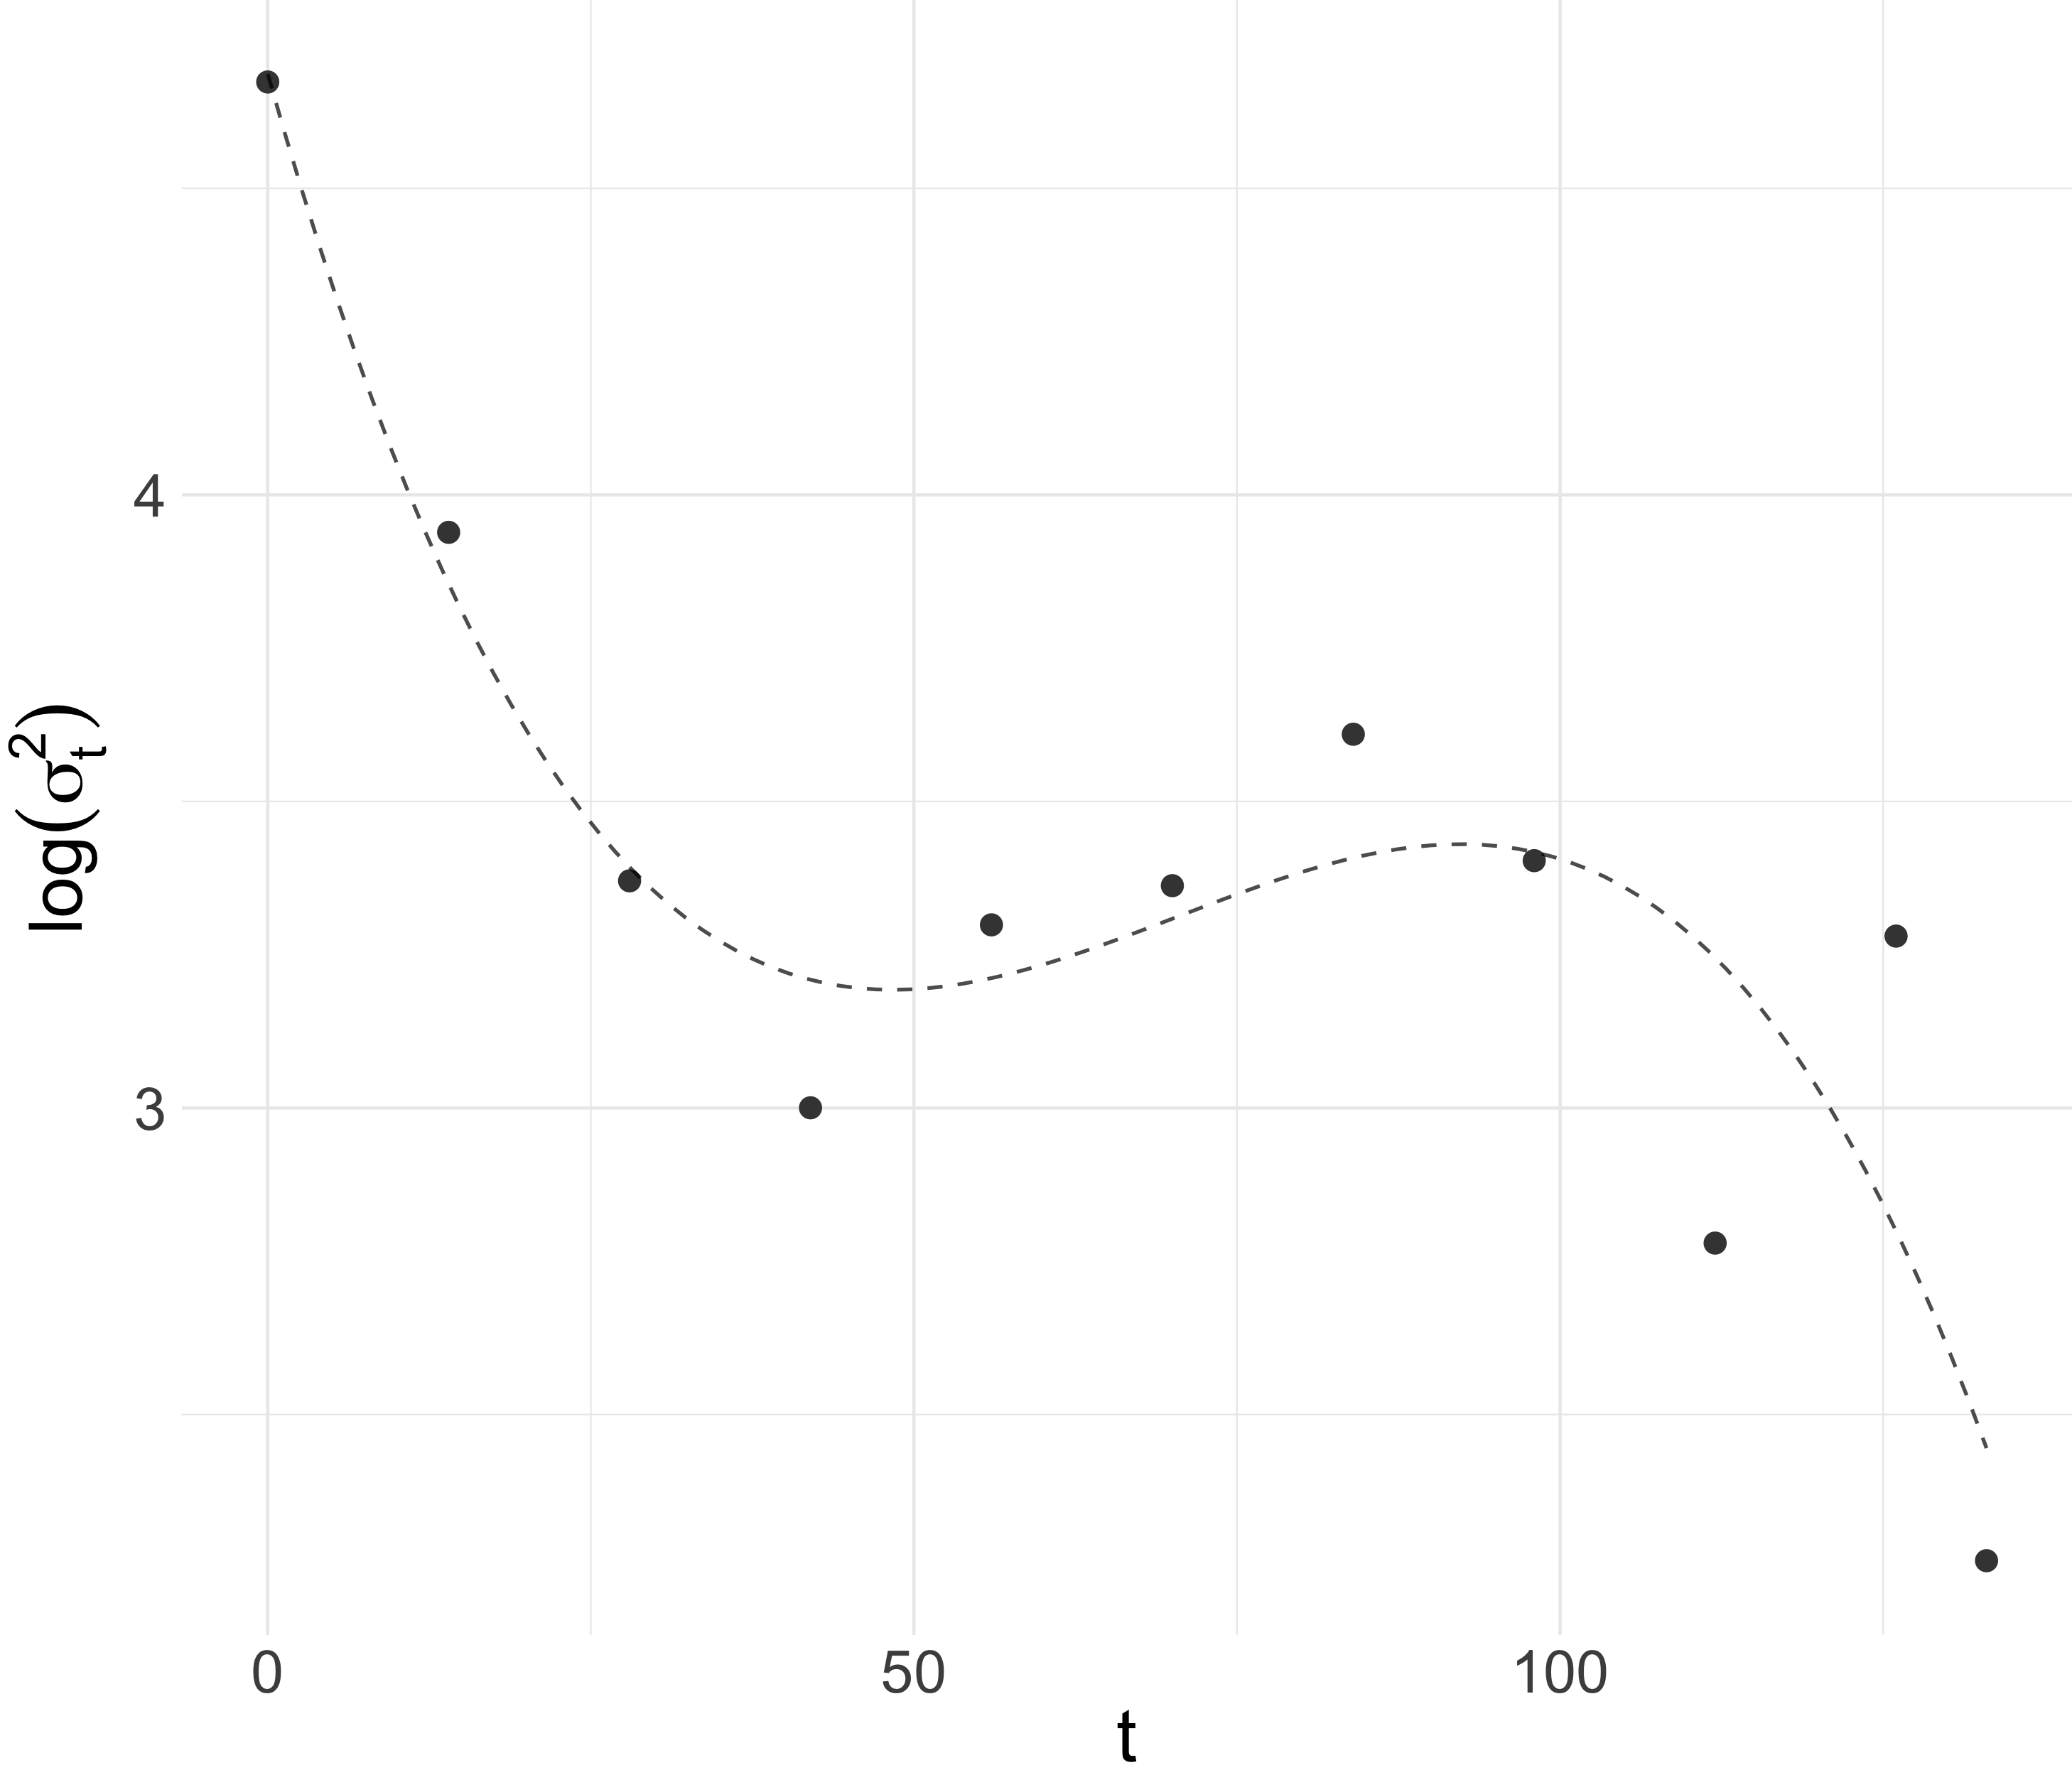
\includegraphics[width=4.5cm]{img/cattle/cattleA-innovariogram-with-cubic-smooth}};
		\node[right] (red) at (7.5,5.5) {\footnotesize\textcolor{red}{Well tempered neutralino}};
		\node[right] (cya) at (7.5,4.5) {\footnotesize\textcolor{cyan}{$h^0$ resonance}};
		\node[right] (blu) at (7.5,3.5) {\footnotesize\textcolor{blue}{slepton co-annihilations}};
		\node[right] (gre) at (7.5,2.5) {\footnotesize\textcolor{green}{$A^0$ resonance}};
		\node[right] (mag) at (7.5,1.5) {\footnotesize\textcolor{magenta}{stop co-annihilations}};
%		\node[left] at (10,0) {ten_zero};
%		\node[left] at (10,8) {ten_eight};
		\node (cyadot) at (4,3.5) {};
		\node (bludot) at (3.5,2.5) {};
		\node (gredot) at (6,2.5) {};
		\node (magdot) at (3,1.3) {};
		\path[->, color=cyan, line width=1.5] (cya) edge [out = 170, in = 45] (cyadot);
		\path[->, color=blue, line width=1.5] (blu) edge [out = 180, in = 45] (bludot);
		\path[->, color=FlipGreen, line width=1.5] (gre) edge [out = 170, in = 45] (gredot);
		\path[->, color=magenta, line width=1.5] (mag) edge [out = 185, in = 15] (magdot);
	\end{tikzpicture}
\end{frame}


%
%\begin{frame}[c]{Parameter space scan}
%	% This is a template for Flip's Beamer theme. Features:
%	
%	\begin{center}
%	\begin{tikzpicture}%[show background grid] %% Use grid for positioning, then turn off
%		\node at (5,6) {\large \textbf{Direct Detection}};
%		\node [inner sep=0pt,above right] 
%			{\includegraphics[width=9cm]{\scan}};
%		\node[rotate=90] at (.25,3.5) {\footnotesize $\sigma$ [cm$^2$]};
%		\node at (5,.25) {\footnotesize$m_\chi$ [GeV]};
%		\node[right] at (8.8,4.2) {\footnotesize XENON};
%		\normalsize
%		\node[rotate = 15, fill=blue, rounded corners] at (4,3) {
%		\footnotesize
%		\textcolor{white}{$500<f<700$ GeV}
%		};
%		\node[rotate = 15, fill=magenta, rounded corners] at (5.5,2.7) {
%		\footnotesize
%		\textcolor{white}{$700<f<800$ GeV}
%		};
%		\node[rotate = 15, fill=green, rounded corners] at (6.5,2.3) {
%		\footnotesize
%		\textcolor{white}{$800<f<900$ GeV}
%		};
%		\node[rotate = 0, fill=lager, rounded corners] at (9,1.7) {
%		\footnotesize
%		\textcolor{white}{$900<f<1000$ GeV}
%		};
%		\node[right]  at (4,5) {\comment{Ruled out}};
%	\end{tikzpicture}
%	\end{center}
%	\normalsize 
%		
%
%	% \footnotesize\textcolor{Comment}{1104.3572}
%\end{frame}


% {
% \setbeamercolor{background canvas}{bg=black}
% \setbeamercolor{normal text}{bg=red!12}
% \beamertemplateshadingbackground{yellow!50}{magenta!50}
% \begin{frame}{Test}
% 	% \setbeamertemplate{background canvas}[vertical shading][bottom=red!20,top=yellow!30]
% 	
% 	
% 	\textcolor{white}\Large Test
% \end{frame}
% }



\begin{frame}[c]{Miscellaneous}
	\begin{itemize}
		\item Use \texttt{\textbackslash only<2>} to only show something for one overlay
		\item Can also use \texttt{<2->}
		\item For example, can \only<2->{\textcolor{ALERT}{highlight}} highlight a word
		\item If you use \texttt{\textbackslash uncover<3->} you get a \uncover<3->{\textcolor{Alert}{space}} ... see?
		\item Protip: use \texttt{\textbackslash textbackslash} to get a backslash
	\end{itemize}
\end{frame}



\begin{frame}[c]{Problems and Kludges}{Things to work on}
	\begin{itemize}
		\item There seems to be a bug in Beamer where the footnote color (defined using \texttt{setbeamercolor\{footnote\}} and \texttt{setbeamercolor\{footnote mark\}}) contaminates the normal text color. For now I suggest not using footnotes. \comment{They're of questionable use in a talk, anyway.}
		\item Even though comment text is footnote-sized, it still has normal text line spacing. The \texttt{setspace} environment can fix this, but it forces a newline and it seems to make footnotes disappear. 
		\item Make color theme more uniform and based on palette colors.
		% \item It seems like \texttt{setbeamertemplate} can only be used once, subsequent calls are ignored. This means that you can't use a custom background on a single slide. This seems to be due to \textit{XeLaTeX}. % http://tex.stackexchange.com/questions/29497/xelatex-preventing-beamer-from-using-different-backgrounds
	\end{itemize}
\end{frame}


%% Not quite fixed 
\setbeamertemplate{background canvas}[vertical shading][bottom=keynotebottom, middle=keynotemiddle, top=keynotetop]
\begin{frame}[c]{Problems and Kludges}{XeLaTeX, LuaLaTeX}
	 
	XeLaTeX doesn't allow one to use \texttt{setbeamertemplate[background canvas]} multiple times (e.g. to have one slide with a different background). A fix is to include \texttt{\textbackslash def \textbackslash pgfsysdriver\{pgfsys-dvipdfmx.def\} } before the \texttt{documentclass}, but this ends up breaking the arrows pointing to nodes.
	
	In principle, LuaLaTeX can solve this, but that also requires some work since it only looks at Open Type Fonts (e.g. Gill Sans is not available by default).
	
	\comment{\url{http://tex.stackexchange.com/questions/29497/xelatex-preventing-beamer-from-using-different-backgrounds}}
\end{frame}



\begin{frame}[t]{Acknowledgements}
	I have borrowed heavily (and learned much) from Marco Barisione's \alert{Torino theme}, which can be found one his blog. I have also learned and borrowed from Shawn Lankton's Keynote theme. 
	
	\vspace{1em}
	These can be found at
	\begin{itemize}
		\item \url{http://blog.barisione.org}
		\item \footnotesize{\url{http://www.shawnlankton.com/2008/02/beamer-and-latex-with-keynote-theme/}}
	\end{itemize}
	
	\vspace{1em}
	I've tried to maintain lots of comments in the \texttt{.tex} and \texttt{.sty} files to help other template-designers. At the moment it's all a jumbled mess, though!
\end{frame}



\addtocounter{framenumber}{-1}
\begin{frame}[c]{Extra page: Additional hints}{Look, it doesn't add to the total page count!}
	\begin{itemize}
		\item Be sure to turn off any auto-notifiers (e.g.\ GMail)
		\item Consider using a PDF-to-keynote program; \url{http://www.cs.hmc.edu/~oneill/freesoftware/pdftokeynote.html}.
		\item Don't ever go over time.
		\item TikZ transparency trick: \url{http://www.texample.net/tikz/examples/transparent-png-overlay/}
		\item Use \alert{\texttt{addtocounter\{framenumber\}\{-1\}}} for extra slides (like this one) to prevent it from screwing up the page numbering.
	\end{itemize}
\end{frame}

